    \documentclass[
        fleqn,
        usenatbib,
    ]{mnras}
    \usepackage{
        amsmath,
        amssymb,
        newtxtext,
        newtxmath,
        ae, aecompl,
        graphicx,
        booktabs,
    }
    \usepackage[T1]{fontenc}
    \usepackage[
        labelfont=bf, % caption names are labeled in bold
        font=scriptsize % smaller font for captions
    ]{caption}
    \usepackage[font=scriptsize]{subcaption} % subfigures
    \captionsetup{compatibility=false}

    \newcommand*{\rd}[2]{\frac{\mathrm{d}#1}{\mathrm{d}#2}}
    \newcommand*{\pd}[2]{\frac{\partial#1}{\partial#2}}
    \newcommand*{\md}[2]{\frac{\mathrm{D}#1}{\mathrm{D}#2}}
    \newcommand*{\at}[1]{\left.#1\right|}
    \newcommand*{\abs}[1]{\left|#1\right|}
    \newcommand*{\ev}[1]{\langle#1\rangle}
    \newcommand*{\p}[1]{\left(#1\right)}
    \newcommand*{\s}[1]{\left[#1\right]}
    \newcommand*{\z}[1]{\left\{#1\right\}}
    \DeclareMathOperator*{\argmin}{argmin}
    \DeclareMathOperator*{\argmax}{argmax}
    \DeclareMathOperator*{\med}{med}

\title[Cassini State Capture]{Cassini State Capture}
\author[Y. Su et\ al.]{
Yubo Su$^1$,
Dong Lai$^1$
\\
$^1$ Cornell Center for Astrophysics and Planetary Science, Department of
Astronomy, Cornell University, Ithaca, NY 14853, USA
}

\date{Accepted XXX\@. Received YYY\@; in original form ZZZ}

\pubyear{2019}

\begin{document}\label{firstpage}
\pagerange{\pageref{firstpage}--\pageref{lastpage}}
\renewcommand*{\sectionautorefname}{Section}
\maketitle

\begin{abstract}
    Abstract
\end{abstract}

\begin{keywords}
planet--star interactions % chktex 8
\end{keywords}

\section{Introduction}

The primary result of our paper is \autoref{fig:nonad_3_ensemeble}.

\section{Theory}\label{s:eq}

\subsection{Equations of Motion}

Denote $\hat{s}$ spin of planet, $\hat{l}$ angular momentum of planet, and
$\hat{l}_d$ angular momentum of the surrounding disc. We approximate $S \ll L
\ll L_d$, so $\hat{l}_d$ is approximately constant and $\hat{l}$ experiences
negligible backreaction torque from $\hat{s}$. Much of this treatment borrows
from \citealp{anderson2018teeter} and \citealp{millholland_disk}. We consider
precession equations
\begin{align}
    \rd{\hat{s}}{t} &= \omega_{sl} \p{\hat{s} \cdot \hat{l}}
        \p{\hat{s} \times \hat{l}}\label{eq:dsdt}\\
    \rd{\hat{l}}{t} &= \omega_{ld}\p{\hat{l} \cdot \hat{l}_d}
        \p{\hat{l} \times \hat{l}_d}\label{eq:dldt}.
\end{align}
where
\begin{align}
    \omega_{sl} &\equiv \frac{3k_{qp}}{2k_p} \frac{M_\star}{m_p}
        \p{\frac{R_p}{a_p}}^3 \Omega_p,\label{eq:wsl}\\
    \omega_{ld} &\equiv \frac{3M_d}{4M_\star}\p{\frac{a_p}{r_d}}^3 n
        .\label{eq:wld}
\end{align}
% = 1/(152600 yr) (kp = 6kqp, Mstar = msun, mp = mJ, Rp = RJ, ap = AU, Wp = 2pi
% / (10 days))
% = 1 / (573362 yr) (Md/Mstar = 0.01, ap/rd = 1/30)
In \autoref{eq:wsl}, $k_{qp}$ and $k_p$ are related to the planet's quadrupole
moment and moment of inertia respectively \citep[see][]{lai2018}, $M_\star$ is
the mass of the host star, and $M_p, R_p, a_p, \Omega_p$ are the mass, radius,
semi-major axis and angular spin frequency of the planet respectively.
\autoref{eq:wld} is written for a disk of mass $M_d$ located at characteristic
distance $r_d$ from the host star \citep[see][for a power-law disk
profile]{millholland_disk}, $n \equiv \sqrt{GM_\star/a_p^3}$ is the planet's
orbital mean motion. The three angles formed by the three vectors are notated
\begin{align}
    \theta &\equiv \arccos \hat{s} \cdot \hat{l},\\
    \theta_{sd} &\equiv \arccos \hat{s} \cdot \hat{l}_d,\\
    I &\equiv \arccos \hat{l} \cdot \hat{l}_d.
\end{align}

Let us transform to frame rotating about $\hat{l}_p$ with frequency $g \equiv
-\omega_{ld}\cos I < 0$, where $\hat{l}$ fixed. In this frame, $\hat{l}_p$
also remains fixed and $\hat{s}$ evolves as:
\begin{equation}
    \rd{\hat{s}}{t} = \alpha \p{\hat{s} \cdot \hat{l}}
            \p{\hat{s} \times \hat{l}}
        + g\p{\hat{s} \times \hat{l}_d},
\end{equation}
where $\alpha \equiv \omega_{sl} > 0$ follows standard notation. By defining
$\eta$ and nondimensionalized time $\tau$ as
\begin{align}
    \eta \equiv{}& \frac{\abs{g}}{\alpha}\label{eq:eta},\\
        ={}& 3.75 \p{\frac{k_p}{6k_{qp}}}
            \p{\frac{m_p}{0.001 M_\star}}
            \p{\frac{a_p}{1\;\mathrm{AU}}\frac{R_J}{R_p}}^3
            \p{\frac{2\pi/\p{10\;\mathrm{days}}}{\Omega_p}}\nonumber\\
        &\p{\frac{M_d}{0.01 M_{\star}}}
            \p{\frac{30 a_p}{r_d}}^3
            \p{\frac{n}{2\pi / \p{1\;\mathrm{yr}}}}
            \p{\frac{\cos I}{\cos 5^\circ}},\nonumber\\
    \tau \equiv{}& \alpha t,
\end{align}
we can non-dimensionalize the equation of motion as
\begin{equation}
    \rd{\hat{s}}{\tau} = \p{\hat{s} \cdot \hat{l}}
            \p{\hat{s} \times \hat{l}}
        - \eta\p{\hat{s} \times \hat{l}_d}. \label{eq:dsdt_base}
\end{equation}

Following~\cite{millholland_disk}, we allow $g$ to vary in time owing to a
disk with decaying mass
\begin{equation}
    M_d(t) = M_d(0)e^{-t/t_d}.
\end{equation}
As $\alpha$ is held constant, this equates to $\eta$ decaying as $\rd{\eta}{t} =
-\frac{\eta}{t_d}$ as well. We nondimensionalize:
\begin{align}
    \epsilon \equiv{}& \frac{1}{\alpha t_d},\\
        ={}& 0.015 \p{\frac{k_p}{6k_{qp}}}
            \p{\frac{m_p}{0.001 M_\star}}
            \p{\frac{a_p}{1\;\mathrm{AU}}\frac{R_J}{R_p}}^3\nonumber\\
        &\p{\frac{2\pi/\p{10\;\mathrm{days}}}{\Omega_p}}
            \p{\frac{10\;\mathrm{Myr}}{t_d}},\\
    \rd{\eta}{\tau} ={}& -\epsilon \eta.\label{eq:deta_dt}
\end{align}
\autoref{eq:dsdt_base} and \autoref{eq:deta_dt} together constitute our system
of study.

For analytical work, we adopt spherical coordinate system where $\hat{l} =
\hat{z}$ and $\theta, \phi$ are the polar and azimuthal angle of $\hat{s}$. By
convention, we choose $\hat{l}_z$ at coordinates $\theta = I, \phi = \pi$.
Note that $\p{\cos \theta, \phi}$ form a canonically conjugate pair of variables
describing $\hat{s}$. To derive equations of motion for these canonical
coordinates, we introduce Hamiltonian
\begin{align}
    \mathcal{H}\p{\theta, \phi} &= -\frac{1}{2}\p{\hat{s} \cdot \hat{l}}^2
            + \eta \p{\hat{s} \cdot \hat{l}_d}.\label{eq:H}\\
        &= -\frac{1}{2}\cos^2\theta
            + \eta \p{\cos \theta \cos I - \sin I \sin \theta \cos \phi}.
\end{align}

The equations of motion follow by taking derivatives of $\mathcal{H}$ and agree
with \autoref{eq:dsdt_base}:
\begin{subequations}\label{se:H_eom}
    \begin{align}
        \pd{\phi}{t} = \pd{\mathcal{H}}{(\cos\theta)}
            &= -\cos\theta + \eta\p{\cos I + \sin I \cot \theta \cos \phi},\\
        \pd{(\cos \theta)}{t} = -\pd{\mathcal{H}}{\phi}
            &= -\eta \sin I \sin \theta \sin \phi.
    \end{align}
\end{subequations}
While these equations are numerically stiff owing to the $\cot\theta$ term, they
are the most intuitive description for analytical work.

\subsection{Cassini States}\label{ss:cs}

Spin states satisfying $\rd{\hat{s}}{t} = 0$ are referred to as \emph{Cassini
States} (CSs). There are either two or four solutions, depending on the values
of $\eta, I$. Following standard convention and nomenclature (see
\autoref{fig:cs_locs}), CSs 1, 3, 4 have $\phi = 0, \theta < 0$ and CS2 has
$\phi = \pi, \theta > 0$. Of these, CSs 1, 2, 3 are stable while CS4 is unstable
(this follows from linearization of \autoref{se:H_eom}). When $\eta < \eta_c$,
where
\begin{equation}
    \eta_c \equiv \p{\sin^{2/3}I + \cos^{2/3}I}^{-3/2},
\end{equation}
all four CSs exist, and when $\eta > \eta_c$, only CSs 2, 3 exist
\citep{henrard1987,ward2004I}. The CS obliquities as a function of $\eta$ are
shown in \autoref{fig:cs_locs}.
\begin{figure}
    \centering
    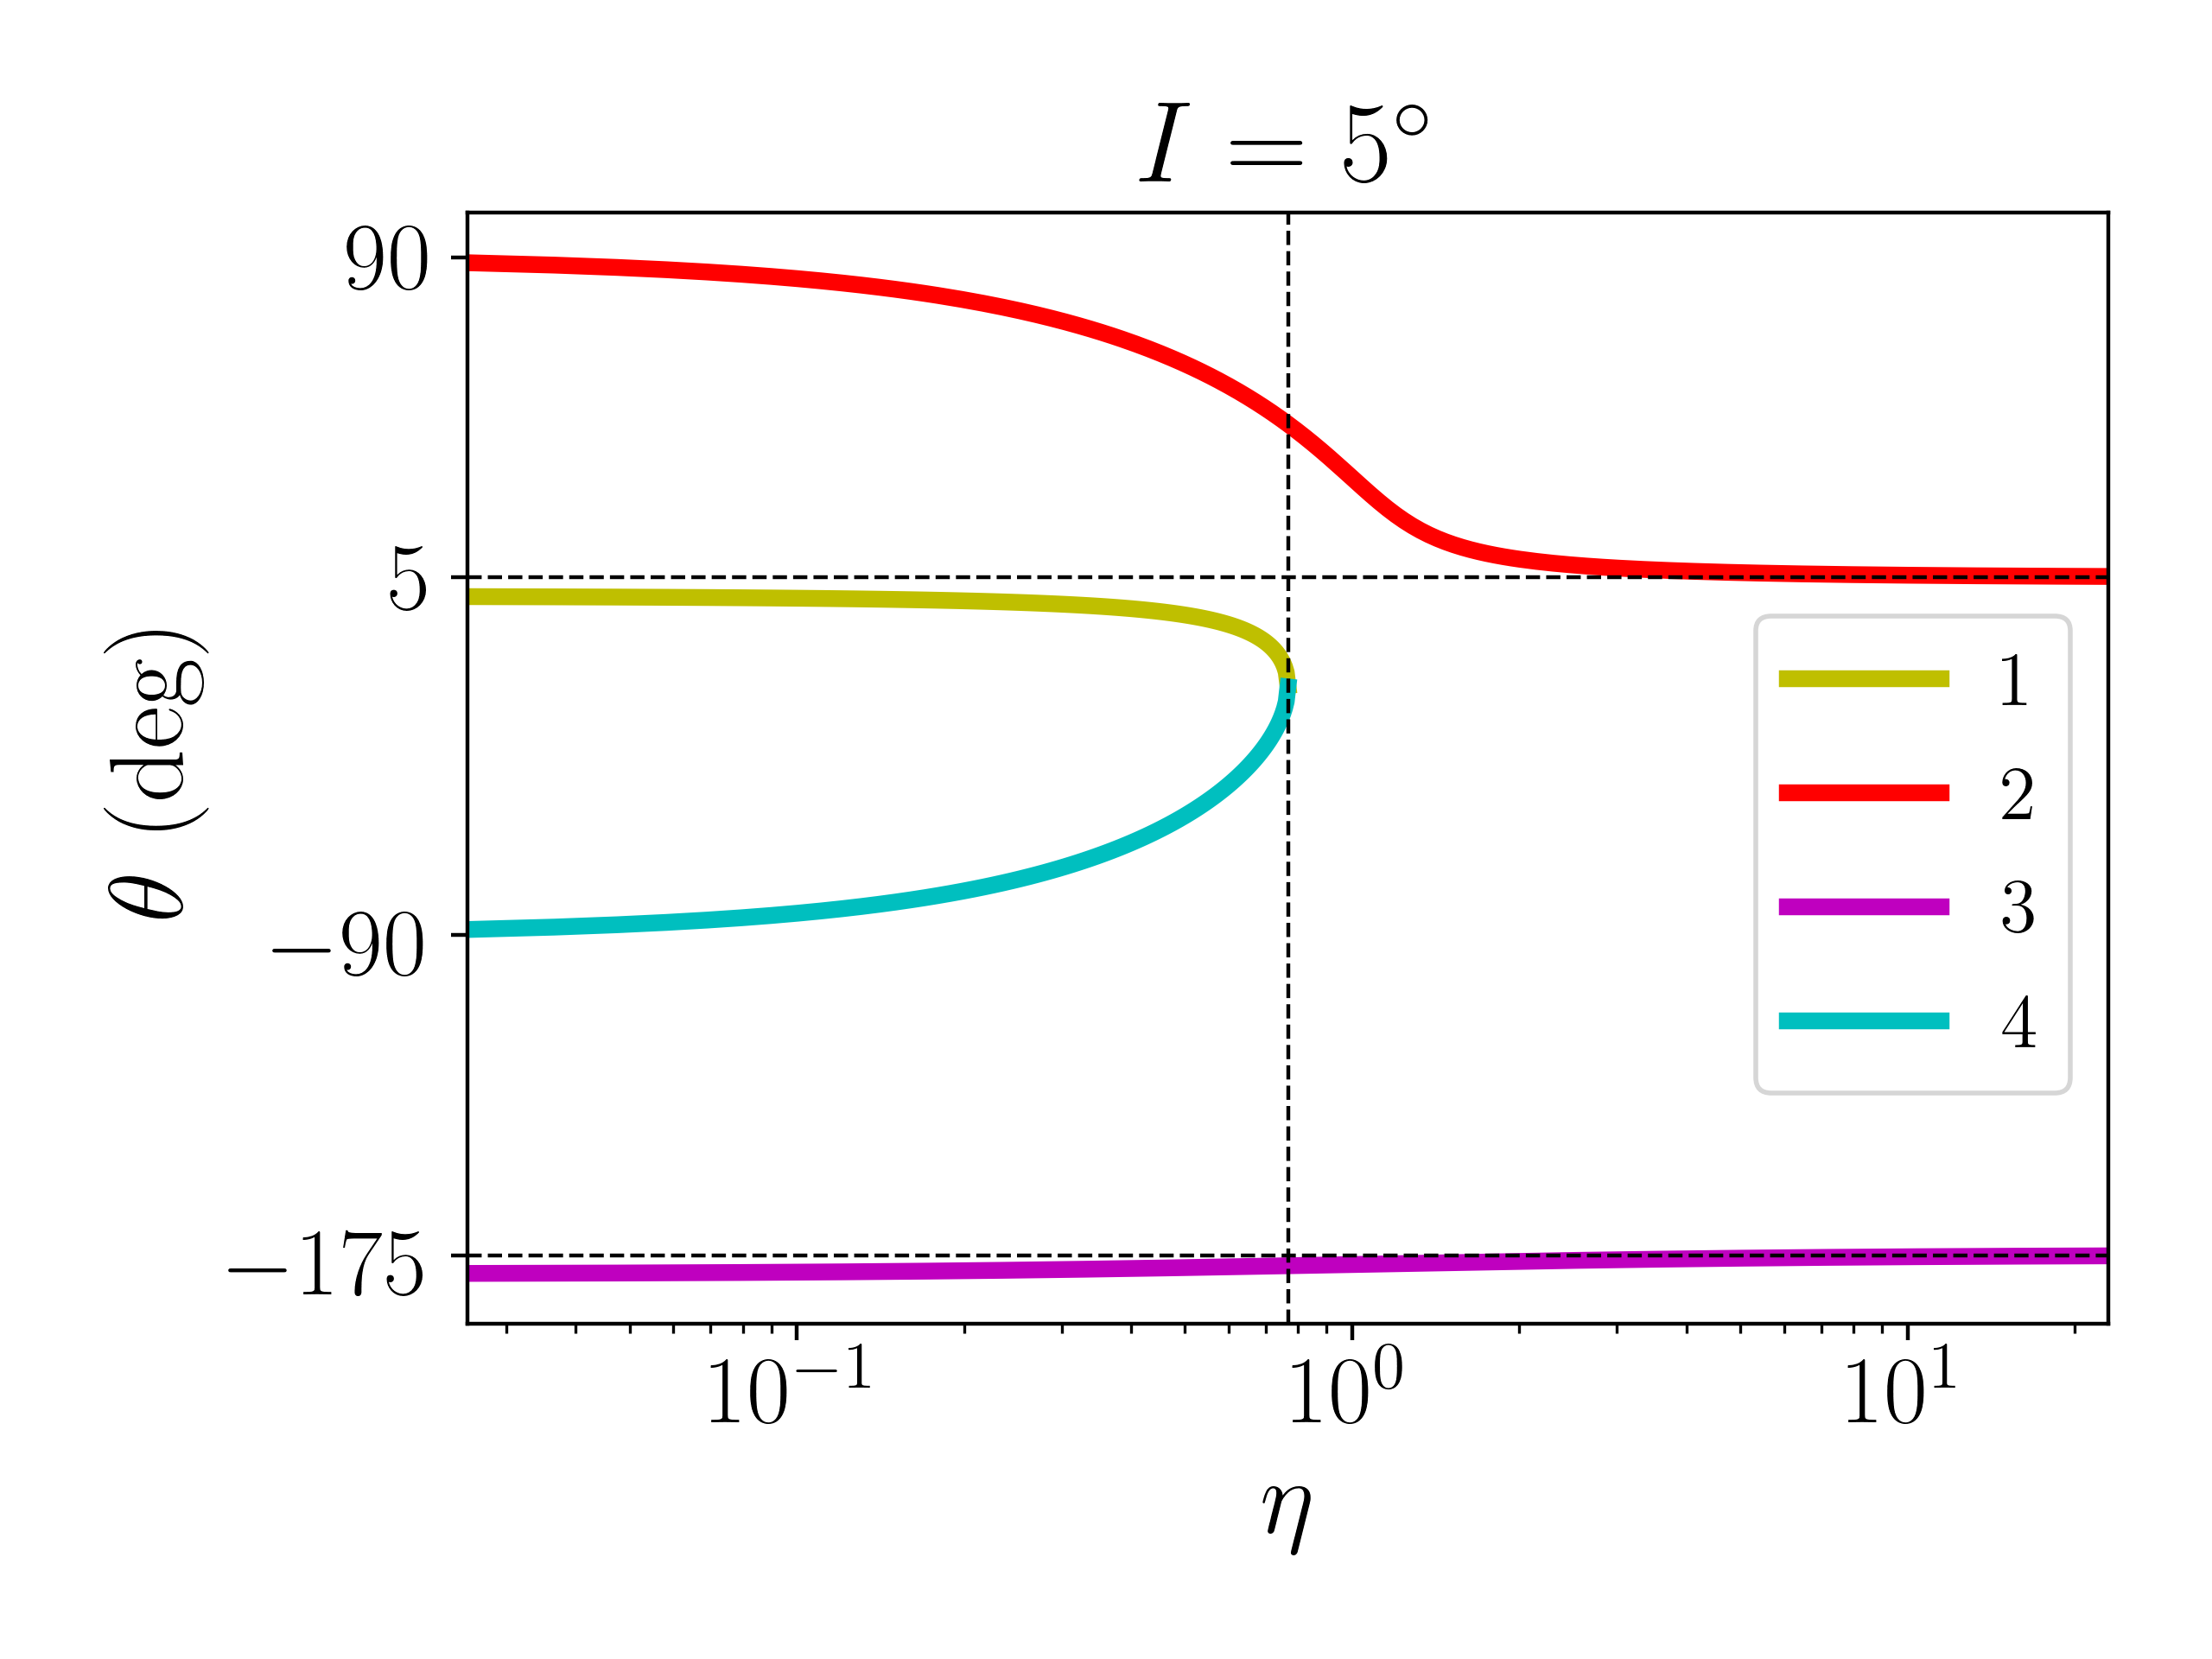
\includegraphics[width=\columnwidth]{../initial/99_misc/2_cs_locs.png}
    \caption{Cassini state obliquities as a function of $\eta$. Note that
    $\theta \in [-\pi, \pi]$ is the traditional definition of the polar angle
    \citep[see e.g.][]{colombo1966,peale1969,henrard1987}.}\label{fig:cs_locs}
\end{figure}

\subsection{Separatrix}

When $\eta < \eta_c$, CS4 exists and is a saddle point. The two trajectories
originating and ending at CS4 are the only two infinite-period orbits in phase
space. Together, these two critical trajectories are referred to as the
\emph{separatrix} and divide phase space into three zones. The separatrix, three
zones, and their relations to the CSs are shown in \autoref{fig:eq_1contours}.
Note that trajectories in zone $II$ librate about CS2 while those in zones
$I$/$III$ circulate.
\begin{figure*}
    \centering
    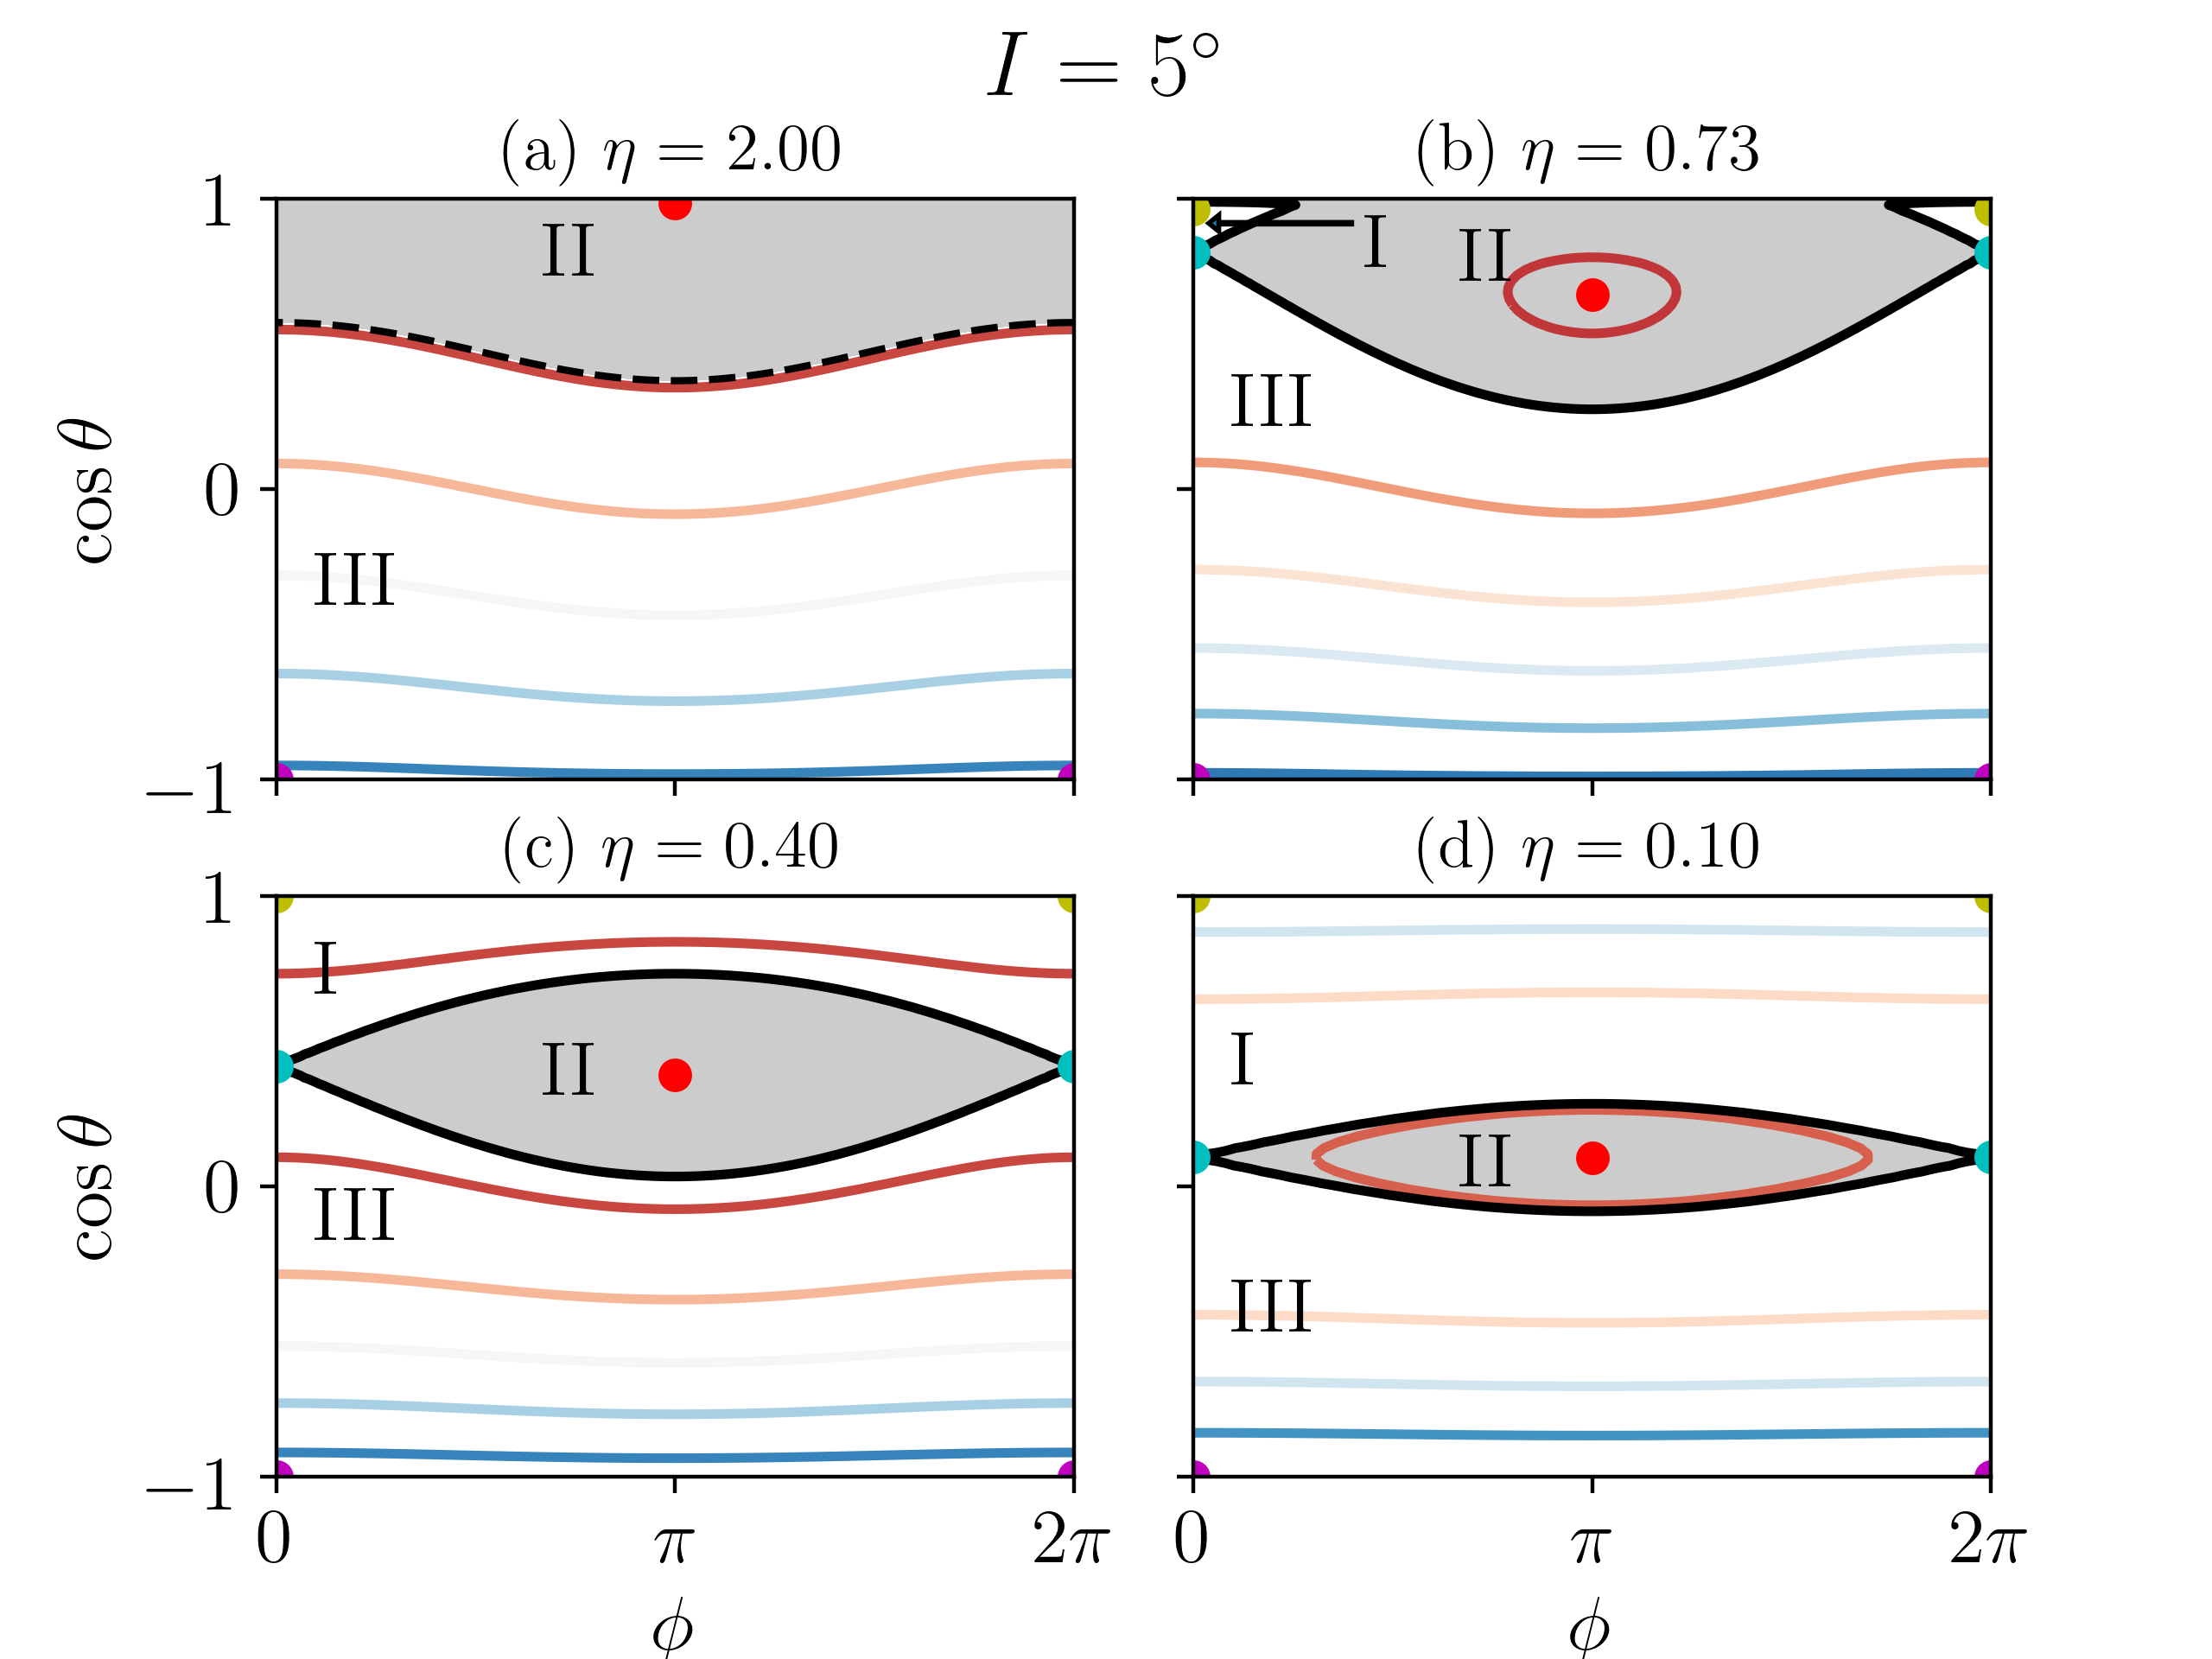
\includegraphics[width=0.8\textwidth]{../initial/0_eta/1contours_flip.png}
    \caption{Contour plot of $\mathcal{H}\p{\phi, \cos \theta}$, where warmer
    colors denote more positive values. The black solid line is the separatrix,
    which only exists for $\eta < \eta_c$. The three zones, divided by the
    separatrix, are labeled. The Cassini states are labeled and have the same
    colors as \autoref{fig:cs_locs}. The interior of the separatrix, shaded in
    grey, is formally only defined for $\eta < \eta_c$, but we may identify the
    phase space trajectories that flow into zone $II$ when evolved forward in
    time; this is the shaded region in the top left plot, bounded by the dotted
    black line.}\label{fig:eq_1contours}
\end{figure*}

The unsigned areas of the three zones are known exactly
\citep{henrard1987,ward2004I}. Defining
\begin{align*}
    z_0 &= \eta\cos I, &
    \chi &= \sqrt{-\frac{\tan^3\theta_4}{\tan I} - 1},\\
    \rho &= \chi \frac{\sin^2 \theta_4\cos \theta_4}{
        \chi^2 \cos^2\theta_4 + 1},&
    T &= 2\chi \frac{\cos \theta_4}{
        \chi^2 \cos^2\theta_4 - 1},\\
\end{align*}
the areas for $\eta < \eta_c$ are given by
\begin{subequations}\label{se:area_ward}
    \begin{align}
        A_{II} &= 8\rho + 4\arctan T - 8z_0 \arctan \frac{1}{\chi},\\
        A_I &= 2\pi\p{1 - z_0} - \frac{A_2}{2},\\
        A_{III} &= 2\pi\p{1 + z_0} - \frac{A_2}{2}.
    \end{align}
\end{subequations}
These are plotted as a function of $\eta$ in \autoref{fig:eq_areas}. Note that
the zones are not formally defined for $\eta > \eta_c$, but a natural extension
exists: evolve an initial point $p$ under adiabatic decrease of $\eta > \eta_c$
until the separatrix appears at $\eta = \eta_c$, then identify $p$ with the zone
it is in at $\eta_c$. Since phase space area is conserved under adiabatic
evolution, this implies $A_i\p{\eta > \eta_c} = A_i(\eta_c)$. This extension is
also reflected in the dashed boundary in \autoref{fig:eq_1contours}.
\begin{figure}
    \centering
    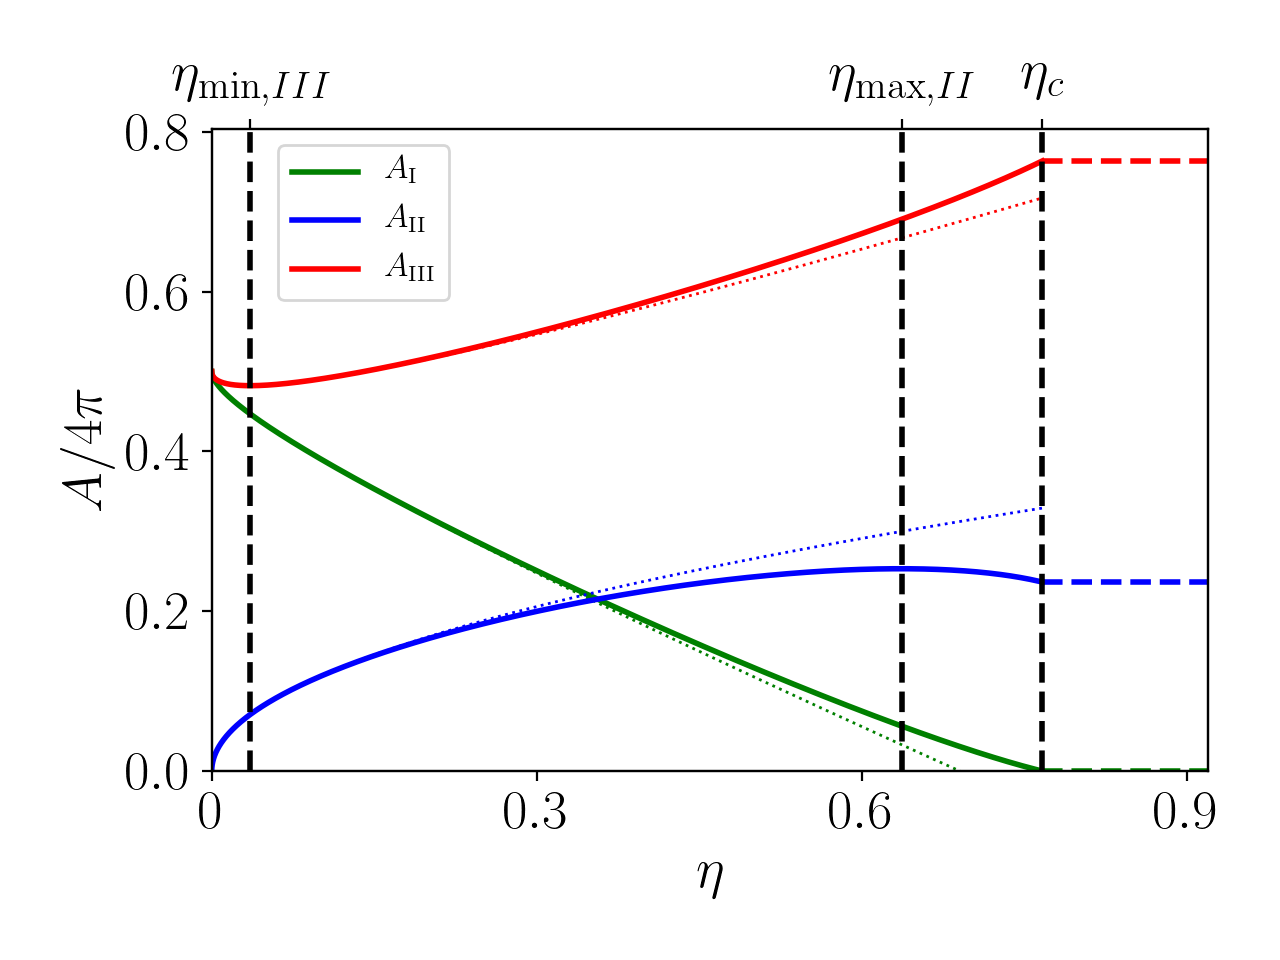
\includegraphics[width=\columnwidth]{../initial/99_misc/1_areas.png}
    \caption{Plot of fractional $A_{i}(\eta)$ as given by
    \autoref{se:area_ward}. Dotted lines correspond to small $\eta$
    approximations discussed in \autoref{s:app_transition}. Dashed lines for
    $\eta > \eta_c$ effective values of $A_{II}, A_{III}$ for $\eta > \eta_c$,
    denoting the area of points that would flow into either area under adiabatic
    decrease of $\eta$ to below $\eta_c$.}\label{fig:eq_areas}
\end{figure}

\section{Adiabatic Evolution}\label{s:ad}

A perturbation to a Hamiltonian system is considered \emph{adiabatic} if it is
sufficiently slow compared to all other relevant time scales in the problem.
In the current problem, the slowest time scale is the \emph{separatrix crossing
time scale}: as $\eta$ evolves, a trajectory may encounter the separatrix at
some value $\eta_\star$ which varies depending on its initial condition. If
$\eta$ changes sufficiently little during the separatrix-crossing orbit, the
evolution of the system may be considered adiabatic. The truly adiabatic limit
corresponds to $\epsilon \to 0$; we take $\epsilon = 3 \times 10^{-4}$ unless
otherwise noted.

One criterion for adiabaticity is that the separatrix crossing timescale be
longer than the the resonant libration period \citep{ward2004I}. The resonant
libration period is just the libration period about CS2, which can be found by
linearizing \autoref{se:H_eom} about CS2. This results in constraint
\begin{align}
    -\at{\frac{1}{\eta}\rd{\eta}{\tau}}_{cross} = \epsilon &\lesssim
            \frac{1}{T_{lib}},\nonumber\\
        &\lesssim \frac{1}{2\pi}\sqrt{\eta_\star\sin\theta \sin I
            \p{1 + \eta_\star \frac{\sin I}{\sin^3\theta}}}.\label{eq:ad_constr}
\end{align}
This formula differs from that presented in \citealt{millholland_disk}.

\subsection{Adiabatic Evolution Outcomes}\label{ss:ad_ensemble}

We consider the evolution of a system with arbitrary initial $\theta_{sd, i}
\equiv \at{\theta_{sd}}_{t = 0}$ and $\eta_i \equiv \at{\eta}_{t = 0} \gg 1$. We
are interested in the distribution of final obliquities after $\eta$ decreases
to $\eta_f \ll 1$ (after the disk has dissipated to negligible mass). While it
is likely that $\theta_{sd, i} \approx 0$ as the planet forms in the disk, we
explore all $\theta_{sd, i} \in [0, \pi]$ for completeness.

We evenly sample $101$ values of $\theta_{sd, i}$, and for each $\theta_{sd, i}$
value, we pick $101$ $\hat{s}$ initial conditions approximately on the ring
fixed by $\theta_{sd, i}$\footnote{For each $\theta_{sd, i}$ we choose an
initial condition on the libration cycle with initial condition $\p{\theta_2 +
\theta_{sd, i}, \phi_2}$ (where $\p{\theta_2, \phi_2}$ are the coordinates of
CS2), such that all initial conditions for a given $\theta_{sd, i}$ enclose the
same initial phase space; see \autoref{sss:a_evo}.}. To be concrete, we choose
$\eta_i = 10\eta_c$. For each initial condition, we evolve
Equations~\ref{eq:dsdt_base} and~\ref{eq:deta_dt} until $\eta = 10^{-5}$. For
such small $\eta$, $\hat{s}$ precesses about $\hat{l}$ with uniform final
obliquity $\theta_f$. This transfer function $\theta_f\p{\theta_{sd, i}}$ is our
primary result, and is shown for $I = 5^\circ, 10^\circ, 20^\circ$ in
\autoref{fig:ad_ensemble}, \autoref{fig:3_ensemble_10_35}, and
\autoref{fig:3_ensemble_20_35} respectively. The blue dots represent the results
of the simulation, which are in excellent agreement with the colored tracks.
These colored tracks are calculated semi-analytically using methods explained in
the following section.

\begin{figure}
    \centering
    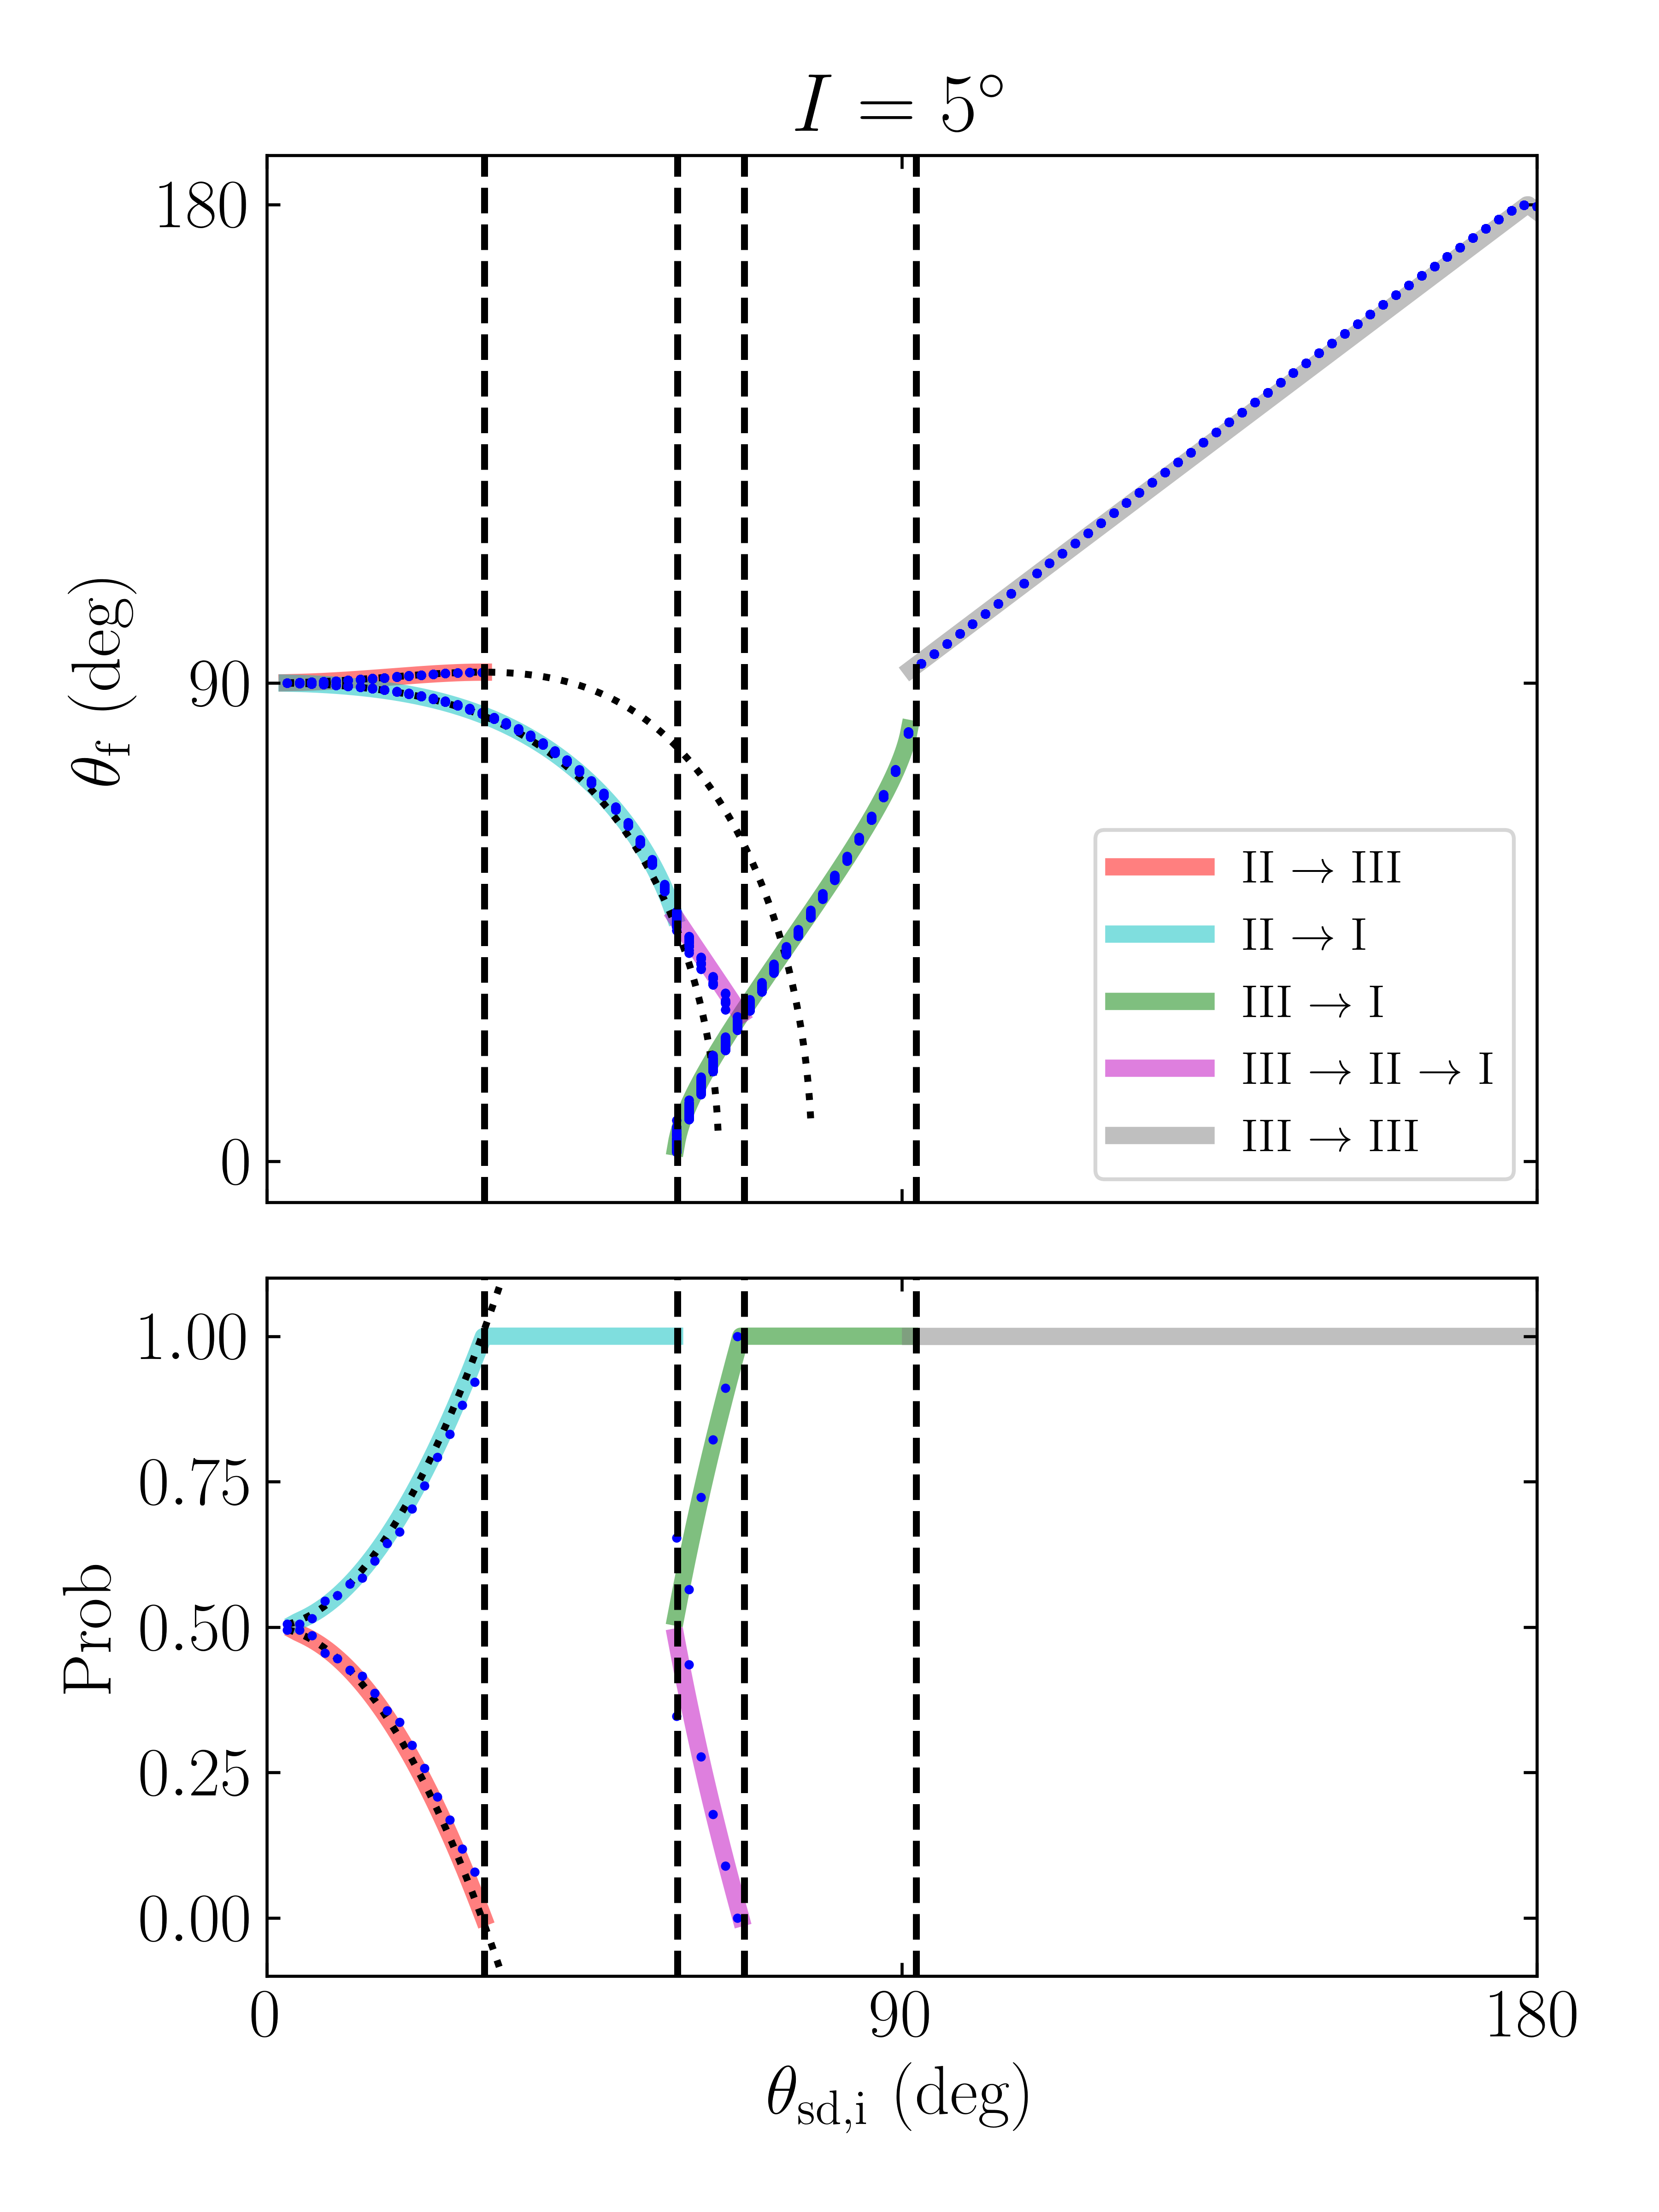
\includegraphics[width=\columnwidth]{../initial/2_toy2/3_ensemble_05_35.png}
    \caption{Top: $\theta_{f}\p{\theta_{sd, i}}$, overlaid with semi-analytic
    predictions of the $\theta_{ f}$ for each of the four nontrivial
    dynamical tracks in colored lines. Black dotted lines correspond to
    small-$\theta_{sd, i}$ predictions derived in \autoref{s:app_transition}.
    Bottom: Semi-analytic probabilities of each of the dynamical tracks for each
    $\theta_{sd, i}$. The five regimes of $\theta_{sd, i}$ values correspond to
    the five regimes of $A_i$ discussed in \autoref{ss:zone_transitions}. Again,
    black dotted lines correspond to simple analytic estimates. Vertical black
    dashed lines correspond to the analytical predictions of where each
    dynamical track is accessible, as described in
    \autoref{ss:zone_transitions}.}\label{fig:ad_ensemble}
\end{figure}
\begin{figure}
    \centering
    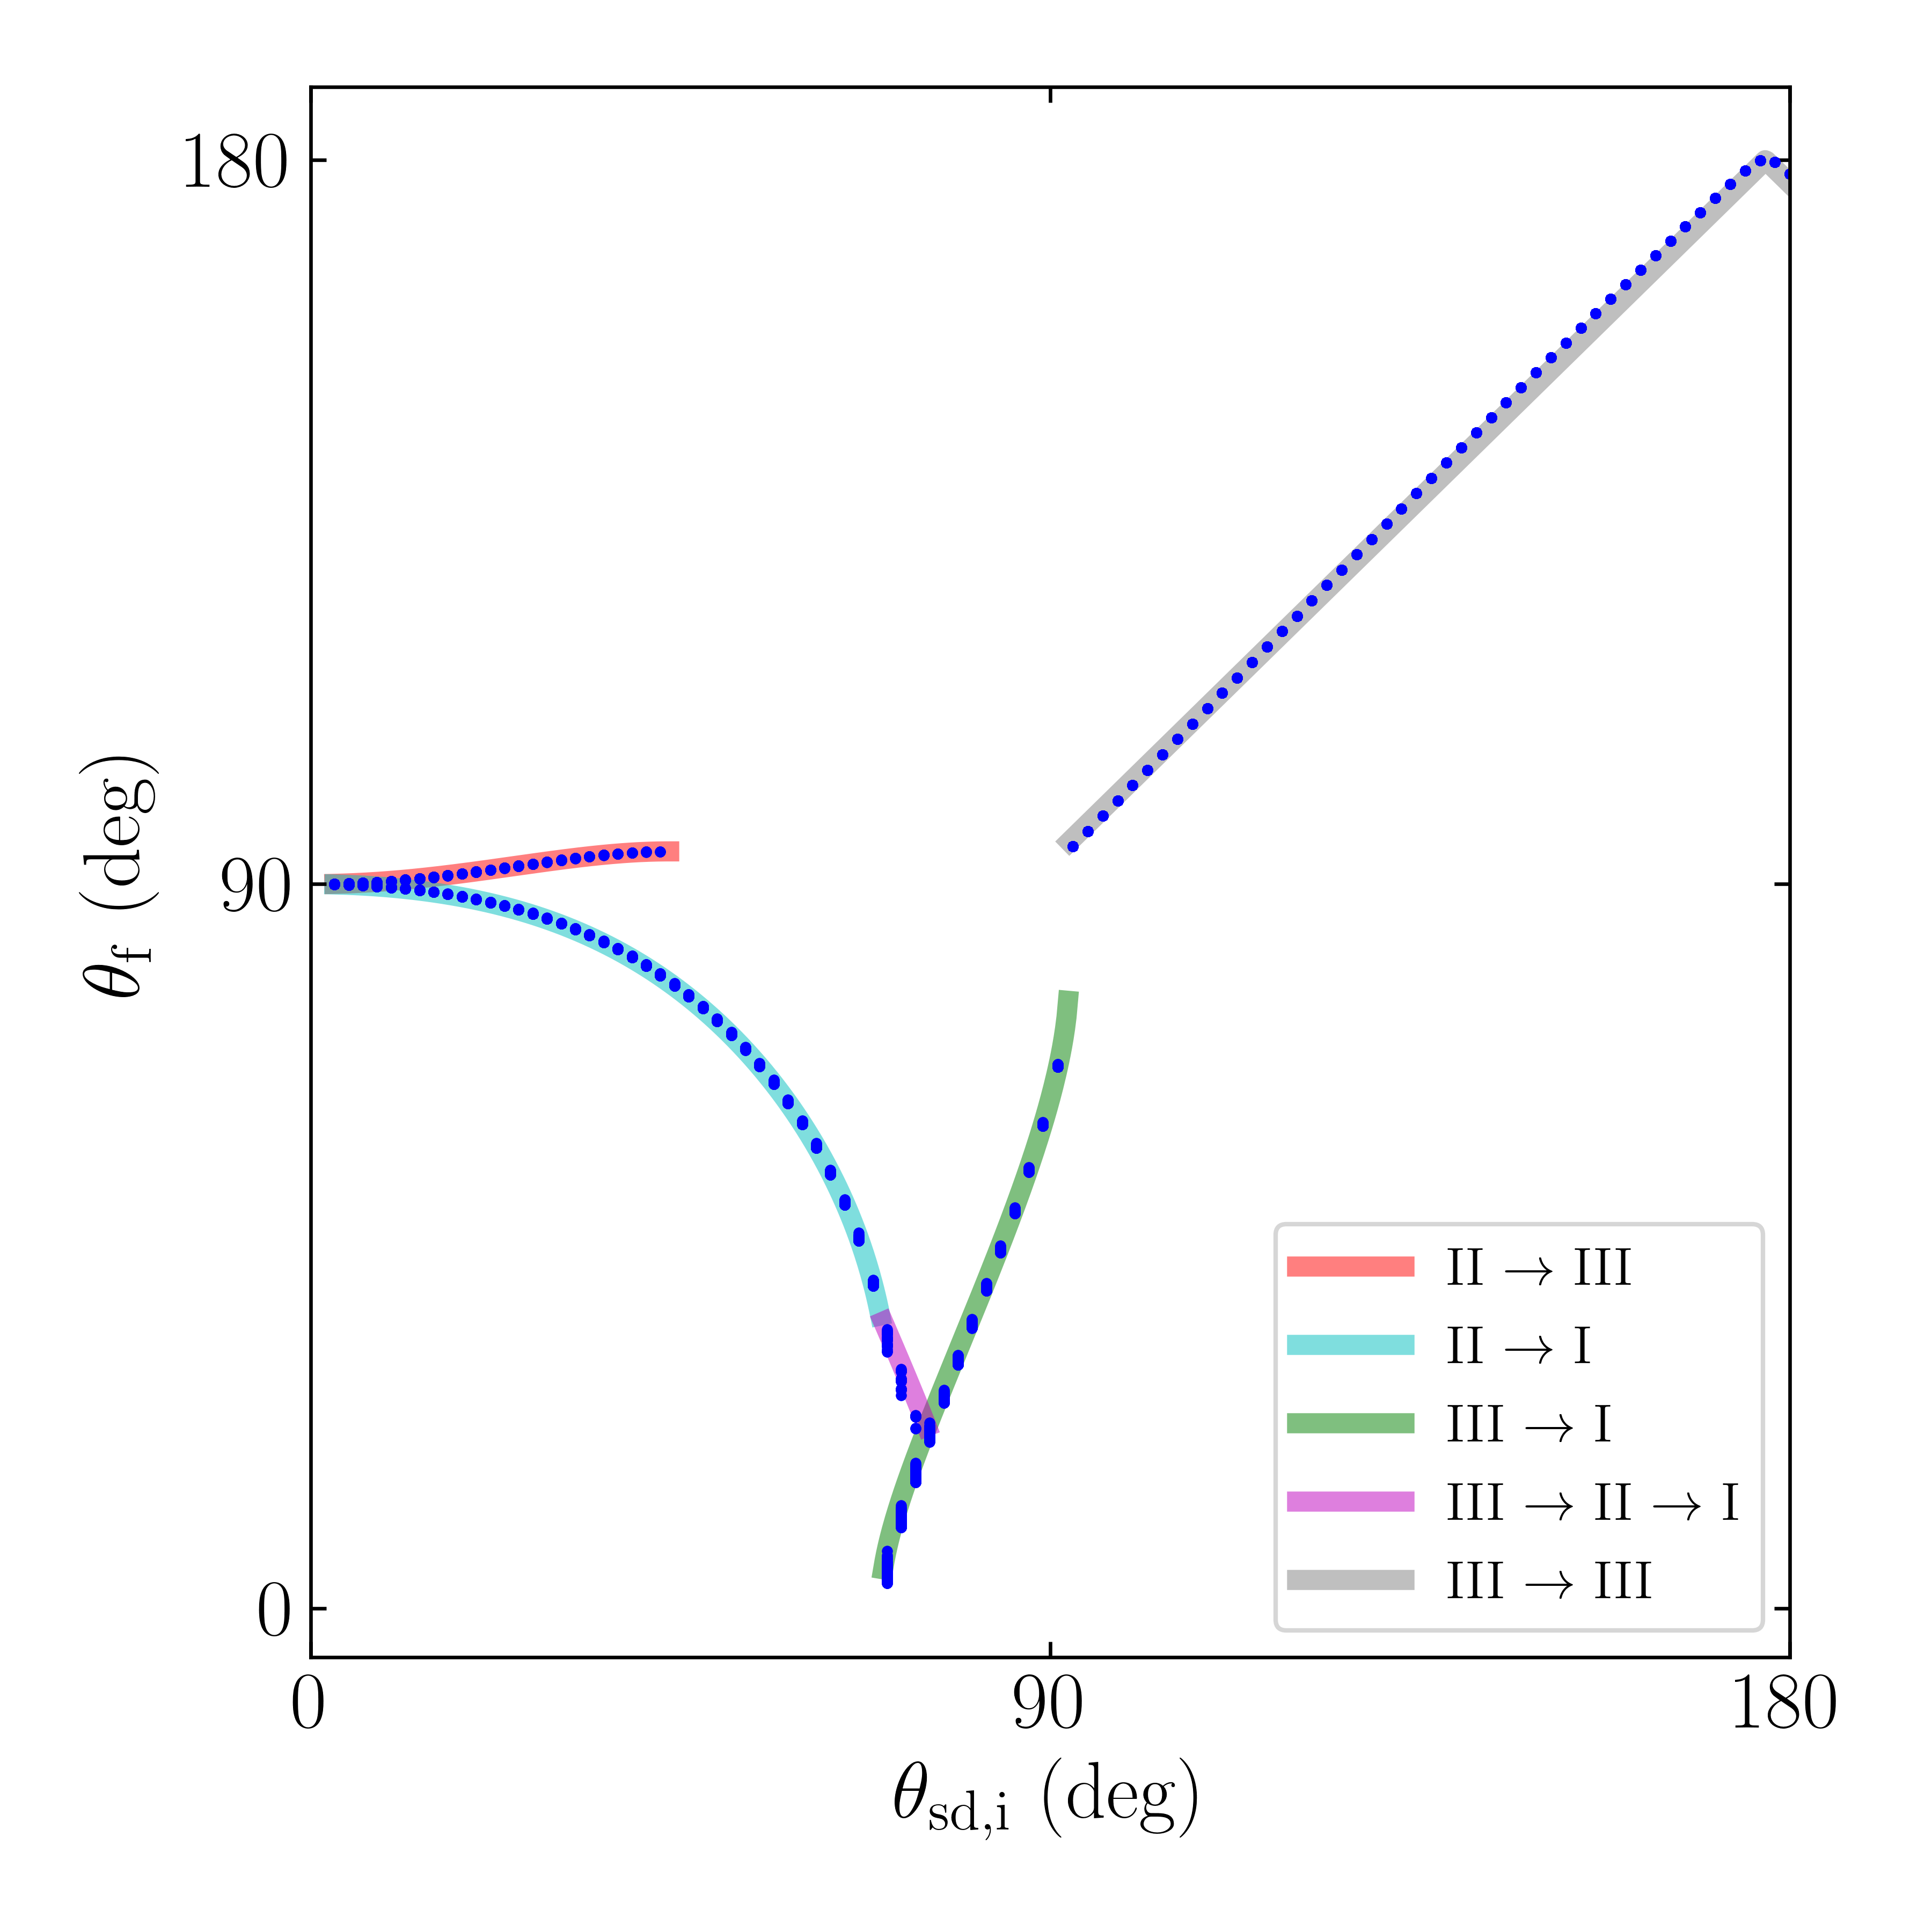
\includegraphics[width=\columnwidth]{../initial/2_toy2/3_ensemble_10_35.png}
    \caption{Same as \autoref{fig:ad_ensemble} but for $I =
    10^\circ$.}\label{fig:3_ensemble_10_35}
\end{figure}
\begin{figure}
    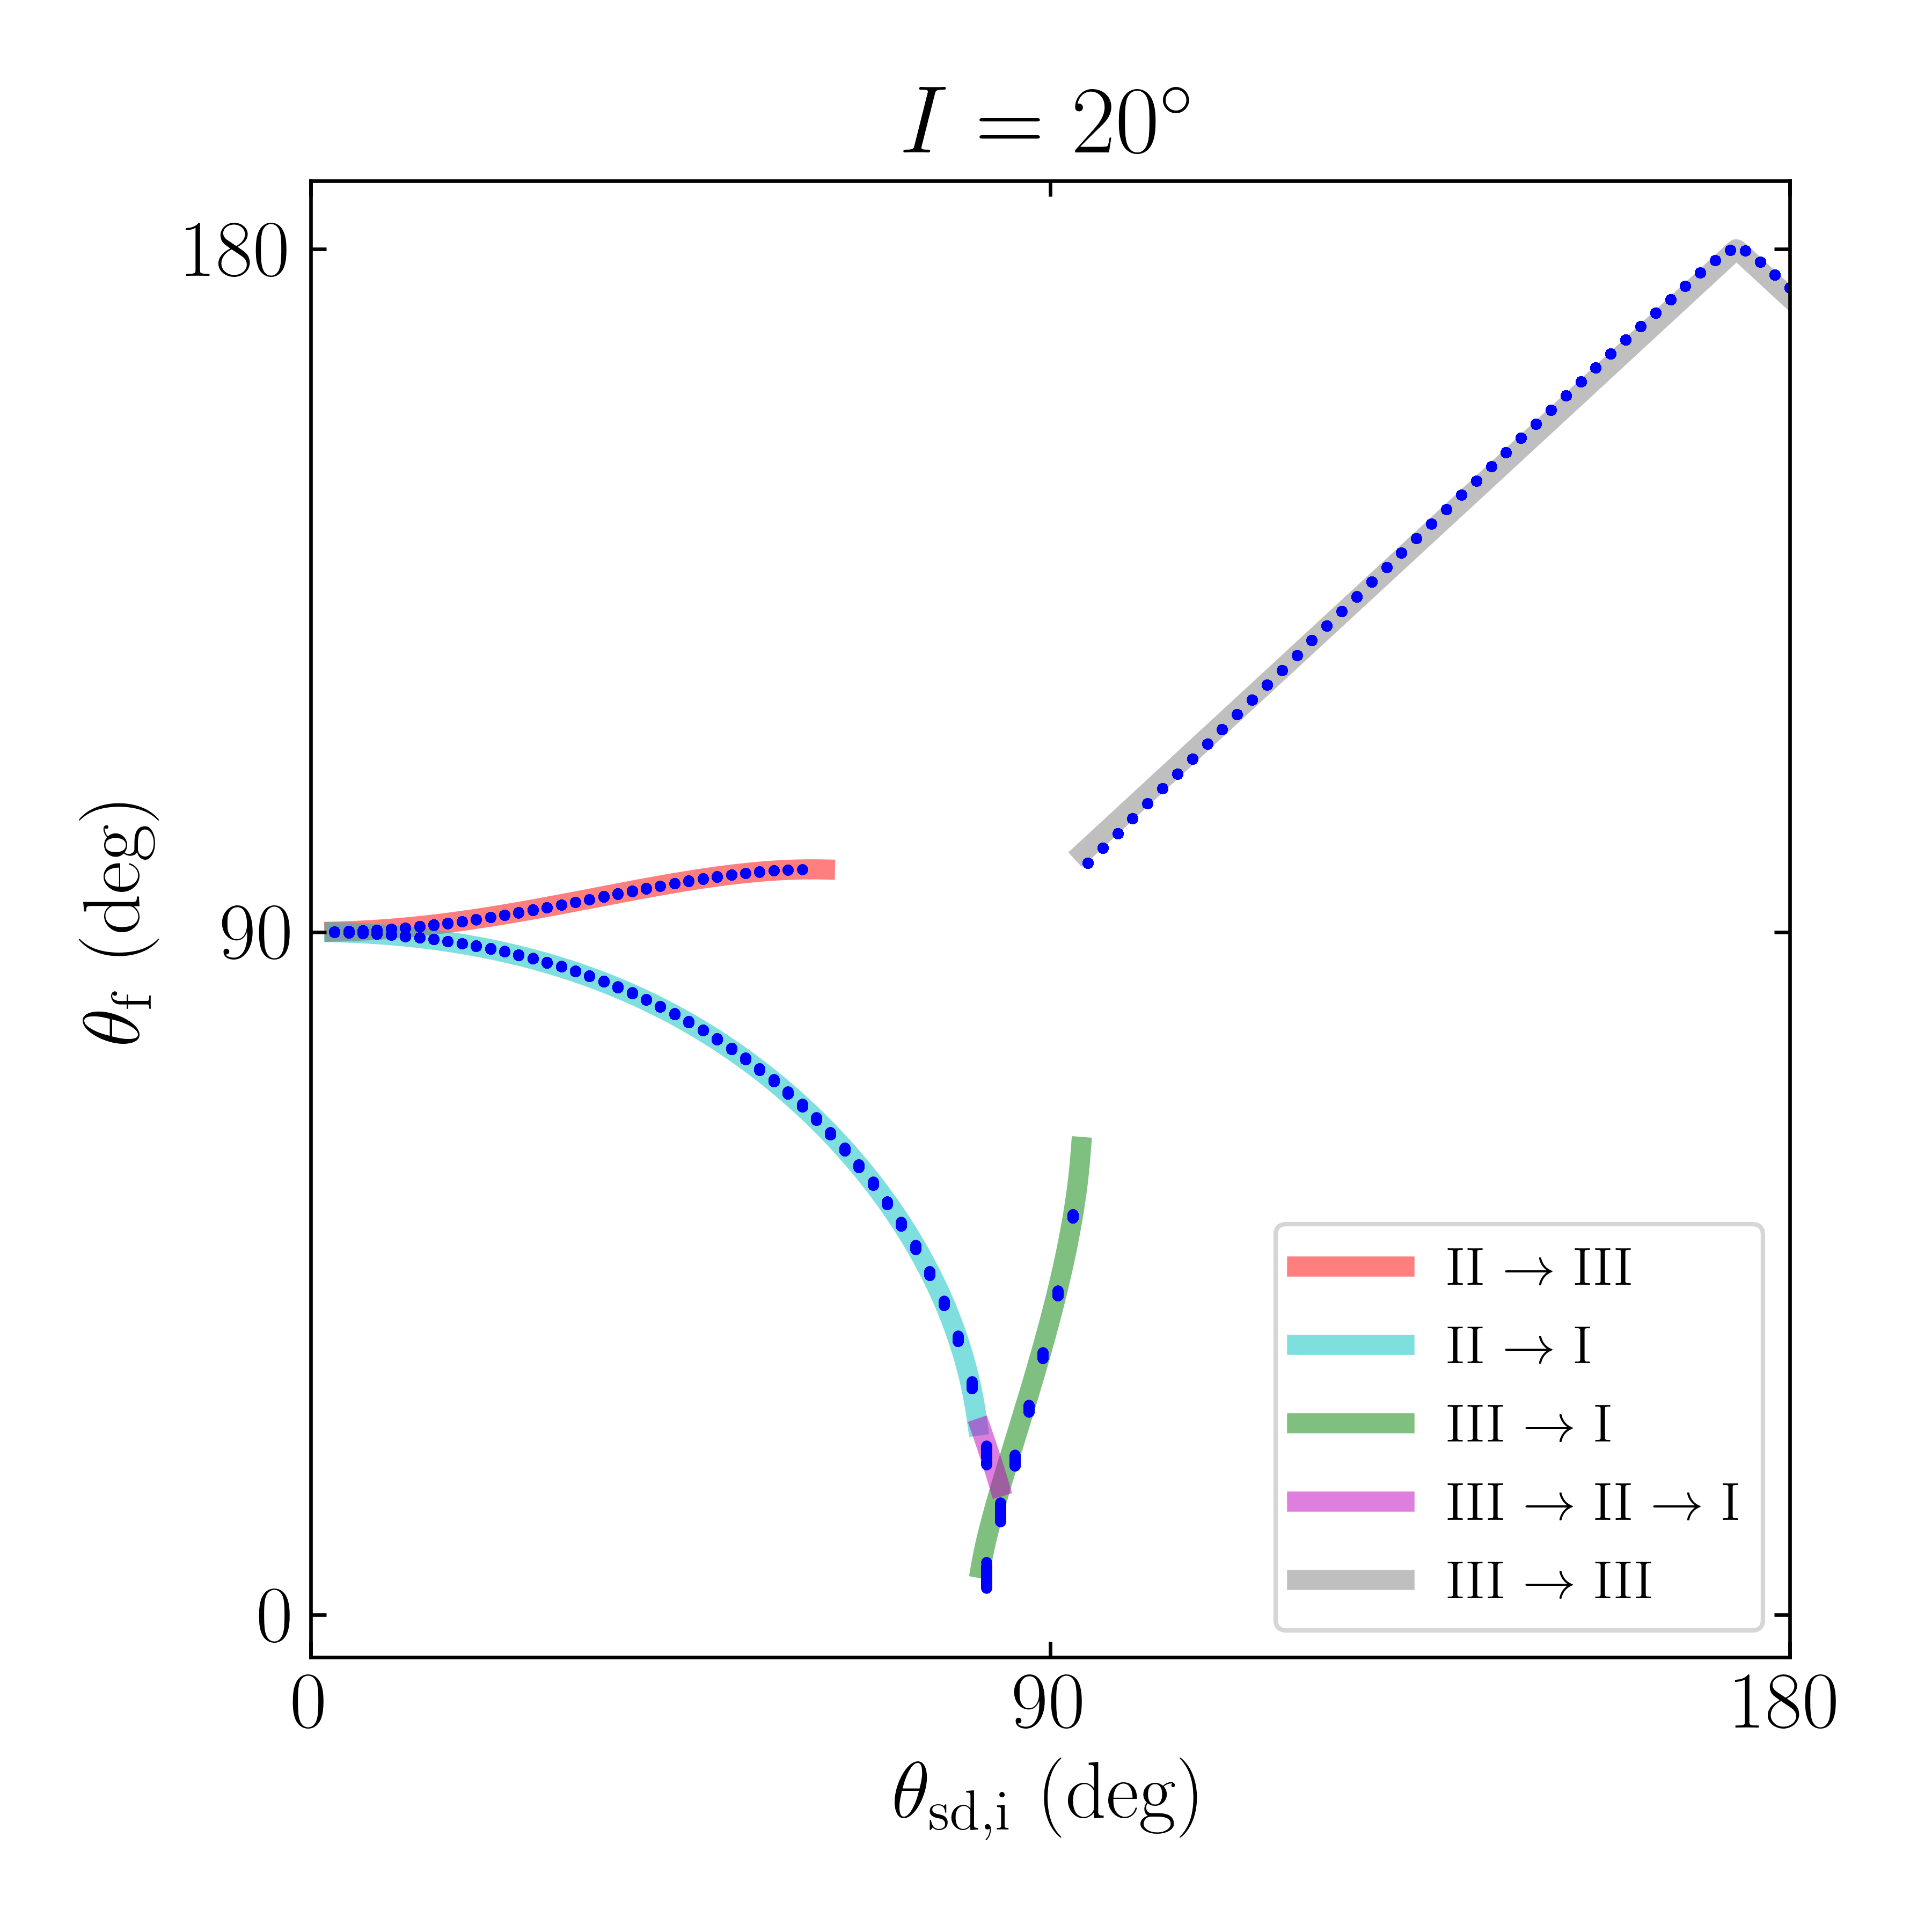
\includegraphics[width=\columnwidth]{../initial/2_toy2/3_ensemble_20_35.png}
    \caption{Same as \autoref{fig:ad_ensemble} but for $I = 20^\circ$. The $III
    \to II \to I$ track is not visible since the maximum $A_{II}$ is very near
    $\eta_c$ for $I = 20^\circ$.}\label{fig:3_ensemble_20_35}
\end{figure}

\subsection{Adiabatic Evolution Theory}\label{ss:zone_transitions}

The evolutionary tracks that govern the behavior of $\theta_f\p{\theta_{sd,
i}}$ correspond to particular sequences of separatrix crossings. Coarsely, they
can be understood using a combination of (i) how the enclosed phase space area
by the trajectory evolves across each separatrix crossing, and (ii) the
associated probabilities with each separatrix crossing.

\subsubsection{Governing Principles: Evolution of $A$}\label{sss:a_evo}

First, we consider how the enclosed phase space area by a trajectory evolves
over time. In the absence of separatrix encounters, the enclosed phase space
area $\oint \cos\theta \;\mathrm{d}\phi$ is an adiabatic invariant. In
particular, we adopt convention where
\begin{equation}
    A \equiv \oint \p{1 - \cos \theta}\;\mathrm{d}\phi.\label{eq:a_oint}
\end{equation}
This definition of $A$ has the advantage of (i) being continuous at $\cos \theta
= 1$, and (ii) being easily expressible as combinations of the $A_i$ of
\autoref{se:area_ward}. The bounds of the integral are either a libration
($\phi$ returns to its original value with the same $\dot{q\phi}$ sign) or
circulation cycle ($\phi$ advances to $\phi \pm 2\pi$). Note lastly that $A$ has
simple physical interpretation of are enclosed on the unit sphere by $\hat{s}$
over one cycle measured relative to $+\hat{z}$:
\begin{equation*}
    \int \int\limits_{\cos \theta(\phi)}^1
        \mathrm{d}\cos\theta\;\mathrm{d}\phi = \int \p{1 - \cos \theta(\phi)}
            \;\mathrm{d}\phi.
\end{equation*}

Observe that when $\eta_i \gg 1$, trajectories librate about $\hat{l}_d$ with
constant $\theta_{sd}$, meaning they enclose initial phase space area
\begin{equation}
    A_i \equiv \at{A}_{t = 0}
        = 2\pi\p{1 - \cos \theta_{sd, i}}.\label{eq:ai_qsd}
\end{equation}
Complications arise when considering finite $\eta_i$, as trajectories near CS2 or
CS3 librate about these equilibria respectively, rather than $\hat{l}_d$, and
\autoref{eq:ai_qsd} is no longer exact. In practice, \autoref{eq:ai_qsd} holds
very well when defining $\theta_{sd, i}$ as the angular distance to CS2; an
exception is discussed in \autoref{sss:evol_traj}.

Beginning at the last separatrix crossing, the final enclosed phase space area
$A_f$ will be conserved for all time. As $\eta \to 0$, trajectories circulate at
constant obliquity $\theta_f$, related to $A_f$ by
\begin{equation}
    2\pi\p{1 - \cos \theta_f} = A_f. \label{eq:qfaf}
\end{equation}

$A$ is not conserved when the trajectory encounters the separatrix. Howover,
its change is easily understood \citep{henrard1982}. In essence, when the
trajectory crosses the separatrix, it continues to evolve adjacent to the
separatrix. So if a separatrix crossing results in a zone I trajectory, the
resultant $A$ can be approximated by integrating \autoref{eq:a_oint} along the
upper leg of the separatrix. Pictorally, this can be seen in the bottom plots of
\autoref{fig:ad_21}.

\subsubsection{Governing Principles: Probabilistic Separatrix Crossing}

When a trajectory experiences separatrix crossing, it transitions into nearby
zones probabilistically. This process is well understood by
\citealp{henrard1982,henrard1987}. Their results may be simply summarized as
follows: if a zone $i$ is shrinking while adjacent zones $j, k$ are expanding
such that the sum of their areas is constant, the probability of transition from
zone $i$ to zone $j$ is given
\begin{align}
    \Pr\p{i \to j} = -\frac{\pd{A_j}{t}}{ \pd{A_i}{t}}
        = -\frac{\pd{A_j}{\eta}}{ \pd{A_i}{\eta}},\\
    \Pr\p{i \to k}
        = -\frac{\pd{A_k}{\eta}}{ \pd{A_i}{\eta}}.\label{eq:henrard_hop}
\end{align}
Note that $\Pr \p{i \to j} + \Pr\p{i \to k} = 1$. This can be used directly in
conjunction with \autoref{se:area_ward} to understand for what initial
conditions each track can be observed and with what probabilities.

As a particular example, consider a system in zone $II$ in panel (d) of
\autoref{fig:eq_1contours}. As $\eta$ decreases, zone $II$ will shrink while
zones $I$ and $III$ will expand until the trajectory. Suppose the trajectory
exits zone $II$ at some $\eta_\star$, then the probability of a $II \to I$
transition is $\Pr\p{II \to I} = -\frac{\dot{A}_{I}}{\dot{A}_{II}}$, while a $II
\to III$ transition occurs with probability $\Pr\p{II \to III} =
-\frac{\dot{A}_{III}}{\dot{A}_{II}}$.

\subsubsection{Evolutionary Trajectories}\label{sss:evol_traj}

Returning to the evolution of $\hat{s}$, we can classify trajectories by the
separatrix encounters experienced. Initially, in the $\eta > \eta_c$ regime,
only zones $II, III$ exist. Conversely, at the end of the simulation when $\eta
\to 0$, only zones $I, III$ exist. Most simply, one might expect four sequences
of transitions between zones (we call these dynamical ``tracks'') to manifest:
from one of $\z{I, III}$ to one of $\z{II, III}$, where $III \to III$ is a
trivial case (no separatrix encounter). In addition to these four tracks, a
fifth track $III \to II \to I$ is observed. Below, we will describe the
evolution of $A$ throughout each of the five tracks, as well as determine the
initial conditions and probabilities associated with each track:
\begin{itemize}
    \item $II \to I$ --- An example trajectory following this track is depicted
        in \autoref{fig:ad_21}. $\hat{s}$ starts librating about CS2 in zone
        $II$, enclosing some initial phase space area $A_i$. The trajectory is
        able to librate without separatrix encounter until $A_{II}(\eta_\star) =
        A_i$. As the trajectory transitions to a circulating trajectory in zone
        $I$ immediately bordering the separatrix, it will encompass
        $-A_I(\eta_\star)$ phase space area. The final $\theta_f$ is then given
        by \autoref{eq:qfaf}.

        This transition can only occur when the initial condition begins in zone
        II, requiring $A_i < A_{II}(\eta_c)$. Note $A_{II}(\eta_c)$ is given in
        closed form in \citealt{ward2004I} but appears to be incorrect. Then, at
        some known $\eta_\star$ satisfying $A_{II}(\eta_\star) = A_i$, the
        trajectory is ejected from the separatrix following
        \autoref{eq:henrard_hop}. Note that since $\pd{A_i}{\eta} < 0$
        everywhere, while $\pd{A_{II}}{\eta} > 0$ at all possible $\eta_\star$
        for an initial condition starting in zone $II$, this track always has
        nonzero probability.

    \item $II \to III$ --- An example trajectory following this track is
        depicted in \autoref{fig:ad_23}. The only difference from the previous
        track is that, upon separatrix encounter, the trajectory follows the
        circulating trajectory in zone $III$ bordering the separatrix, upon
        which it will encompass $A_f = A_I(\eta_\star) + A_{II}(\eta_\star)$.
        The final obliquity is still given by \autoref{eq:qfaf}.

        Again, this track can only occur when $A_i < A_{II}(\eta_c)$, but a
        further constraint arises when we consider the transition probability
        given by \autoref{eq:henrard_hop}. Upon examination of
        \autoref{fig:eq_areas}, it is clear that $\pd{A_{III}}{\eta} > 0$ for
        many $\eta$. Call
        \begin{equation}
            \eta_{\min, III} \equiv \argmin A_{III}(\eta),
        \end{equation}
        then if $\eta_\star > \eta_{\min, III}$ then $\Pr_{II \to III} < 0$.
        This is understood as a forbidden transition, and so $II \to III$ is
        only a permitted dynamical track if $\eta_\star <, \eta_{\min,
        III}$, or $A_i < \min A_{III}$.

    \item $III \to I$ --- This track is depicted in \autoref{fig:ad_31}.
        The trajectory encounters the separatrix when $A_I(\eta_\star) +
        A_{II}(\eta_\star) = A_i$, upon which it transitions to a zone $I$
        trajectory enclosing $A_f = -A_I$. Then, as always, the final obliquity
        is given by \autoref{eq:qfaf}.

        This track can only occur if $A_i > A_{II}(\eta_c)$, but is also
        constrained by requiring its $A_i$ is sufficiently small it will
        encounter the separatrix (if it is too large, it will never encounter
        the separatrix, which is a $III \to III$ transition). This is written
        $A_i < \max A_I + A_{II} = 4\pi - \min A_{III}$.

        Note that since $\pd{A_I}{\eta} < 0$ always while $\pd{A_{III}}{\eta} >
        0$ for all accessible $\eta_{\star}$, this track is always permitted.

    \item $III \to II \to I$ --- This track is depicted in \autoref{fig:ad_321}.
        The first separatrix encounter occurs at $\eta_1$ when $A_I(\eta_1) +
        A_{II}(\eta_1) = A_i$, upon which the trajectory moves into zone $II$
        enclosing intermediate phase space area $A_m = A_{II}(\eta_1)$.
        Examining \autoref{fig:eq_areas}, there exist values $A$ for which
        $A_{II}(\eta) = A$ has multiple solutions. These are the only values for
        which the $III \to II \to I$ transition is permitted. Thus, as $\eta$
        continues to decrease, a second $\eta_2$ value exists for which $A_m =
        A_II(\eta_2)$, upon which the trajectory is ejected to zone $I$ and $A_f
        = -A_I(\eta_2)$. The final obliquity again then obeys \autoref{eq:qfaf}.

        Similar to the $III \to I$ track, the $III \to II \to I$ track can only
        occur over the same $A_{II}(\eta_c) < A_i < \max A_I + A_{II}$ interval.
        The probability of encountering this track is set by the initial $III
        \to II$ transition. It bears noting that this probability is only
        nonnegative for a very small fraction of $A_i$ values, since it requires
        $\pd{A_{II}}{\eta}$ and $\pd{A_{III}}{\eta}$ to have different signs;
        this occurs only if $A_{II}\p{\eta_c} < A_i < A_{II, \max}$. Outside of
        these bounds, $\Pr_{III \to II} < 0$ which is interpreted again as a
        forbidden transition.

        Then, once a $III \to II$ transition occurs, the second $II \to I$
        transition occurs for some $\eta_2$ satisfying $A_{II}(\eta_2) =
        A_{II}(\eta_1), \eta_2 < \eta_1$. Graphical inspection shows that
        $\pd{A_{II}}{\eta}$ has the same sign as $\pd{A_{III}}{\eta}$ over all
        possible values, so the second $II \to I$ transition is guaranteed,
        completing the $III \to II \to I$ track.

    \item $III \to III$ --- This track depicts the trivial case where no
        separatrix encounter ever occurs, and $A$ is constant throughout the
        evolution. This constraint equates to $A_i > \max A_I + A_{II}$,
        whereupon no separatrix encounter occurs at all, and $A_f = A_i$, which
        for $\eta_i \to \infty, \eta_f \to 0$ results in $\theta = \theta_{sd,
        i}$.

        Note that a small deviation from $\theta = \theta_{sd, i}$ occurs
        because we use finite $\eta_i$, as hinted at in \autoref{sss:a_evo}.
        This is because for $\theta_{sd, i} \gtrsim \pi/2$, trajectories are
        better described as librating about CS3. Nevertheless, we can still
        approximate $A_i$ to good accuracy as the solid angle enclosed by
        libration about CS3 with polar angle $2\pi + \theta_3 - \theta_2 -
        \theta_{sd, i}$. This recovers the correct transfer function
        $\theta_f\p{\theta_{sd, i}}$ for the $III \to III$ regime, as can be
        seen visibly in \autoref{fig:3_ensemble_20_35}.
\end{itemize}
In summary, the five regimes of track possibilities in increasing order of $A_i$
are:
\begin{itemize}
    \item $A_i \in \s{0, A_{II}\p{\eta_{\min, III}}}$: $II \to III, II \to I$
        both possible.

    \item $A_i \in \s{A_{II}\p{\eta_{\min, III}}, A_{II}(\eta_c)}$: $II \to I$
        only.

    \item $A_i \in \s{A_{II}(\eta_c), A_{II, \max}}$: $III \to I, III \to II \to
        I$ both possible.

    \item $A_i \in \s{A_{II, \max}, \max A_I + A_{II}}$: $III \to I$ only.

    \item $A_i > \max A_I + A_{II}$: $III \to III$ only.
\end{itemize}
The corresponding ranges for for $\theta_{sd,i}$ can be computed via
\autoref{eq:ai_qsd}. The boundaries between these ranges are overplotted in
\autoref{fig:ad_ensemble}, where they can be seen to agree well with numerical
results.
\begin{figure}
    \centering
    \begin{subfigure}{\columnwidth}
        \centering
        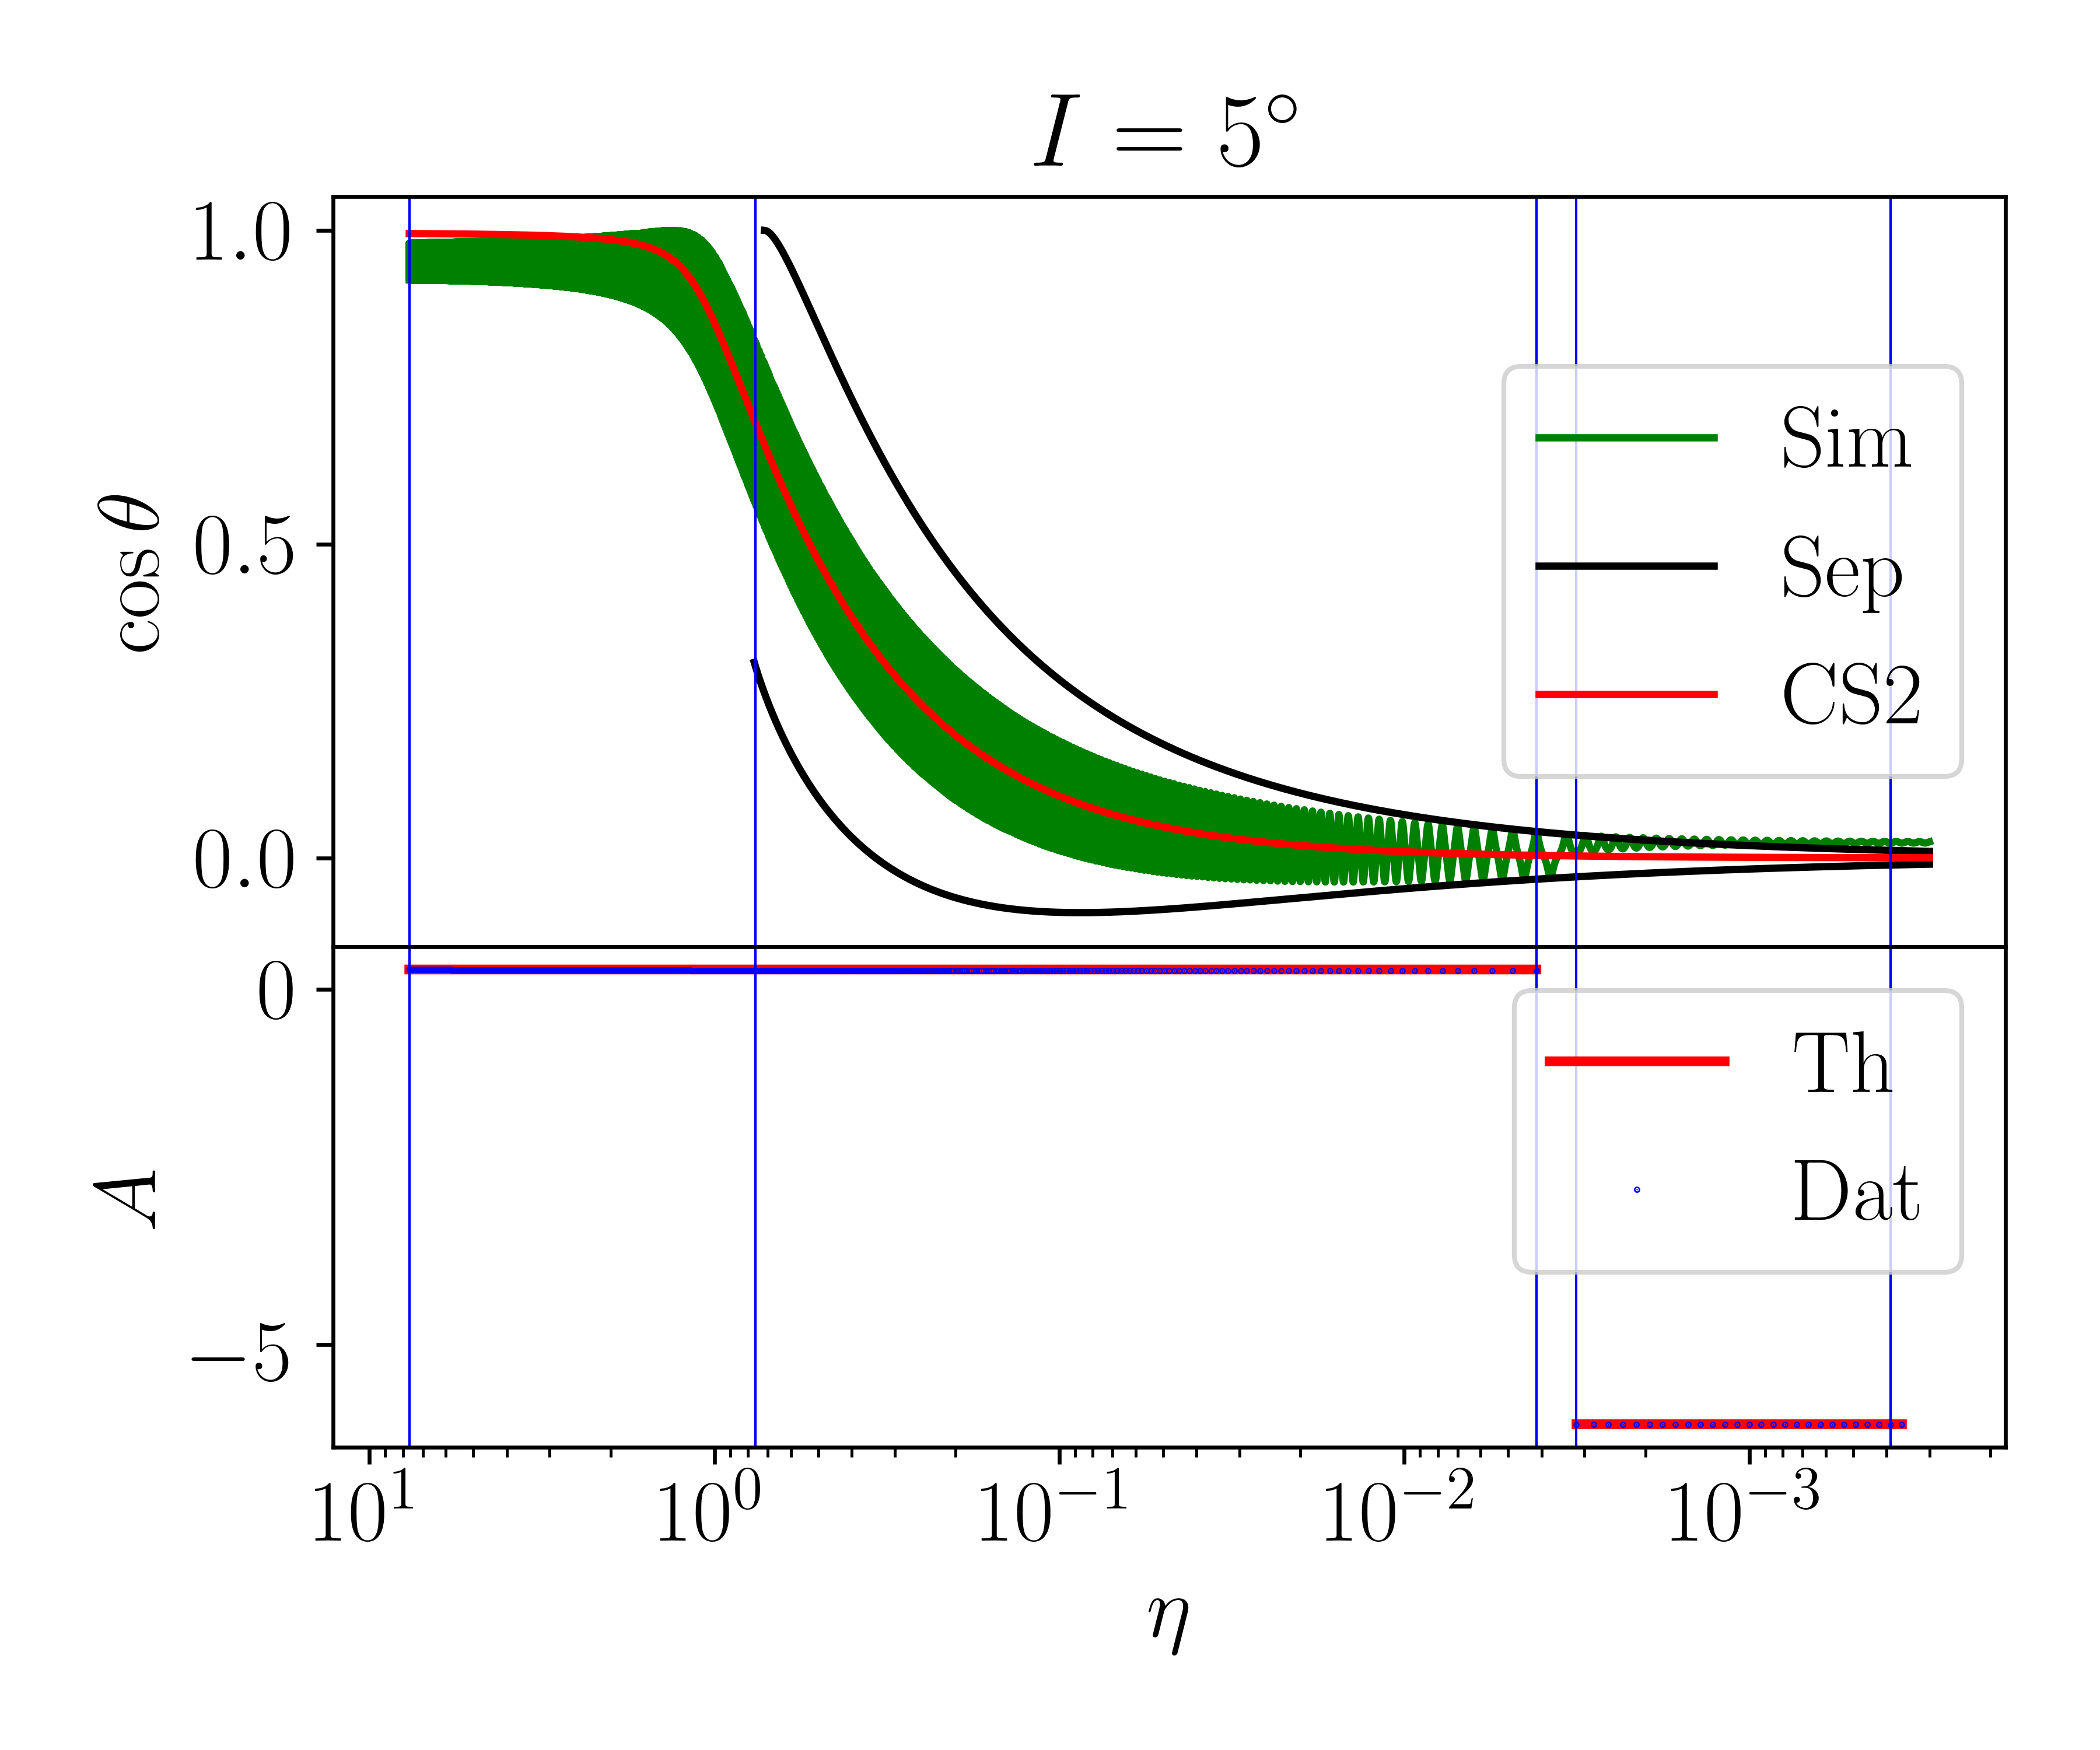
\includegraphics[width=\columnwidth]{../initial/2_toy2/3testo21.png}
    \end{subfigure}
    \begin{subfigure}{\columnwidth}
        \centering
        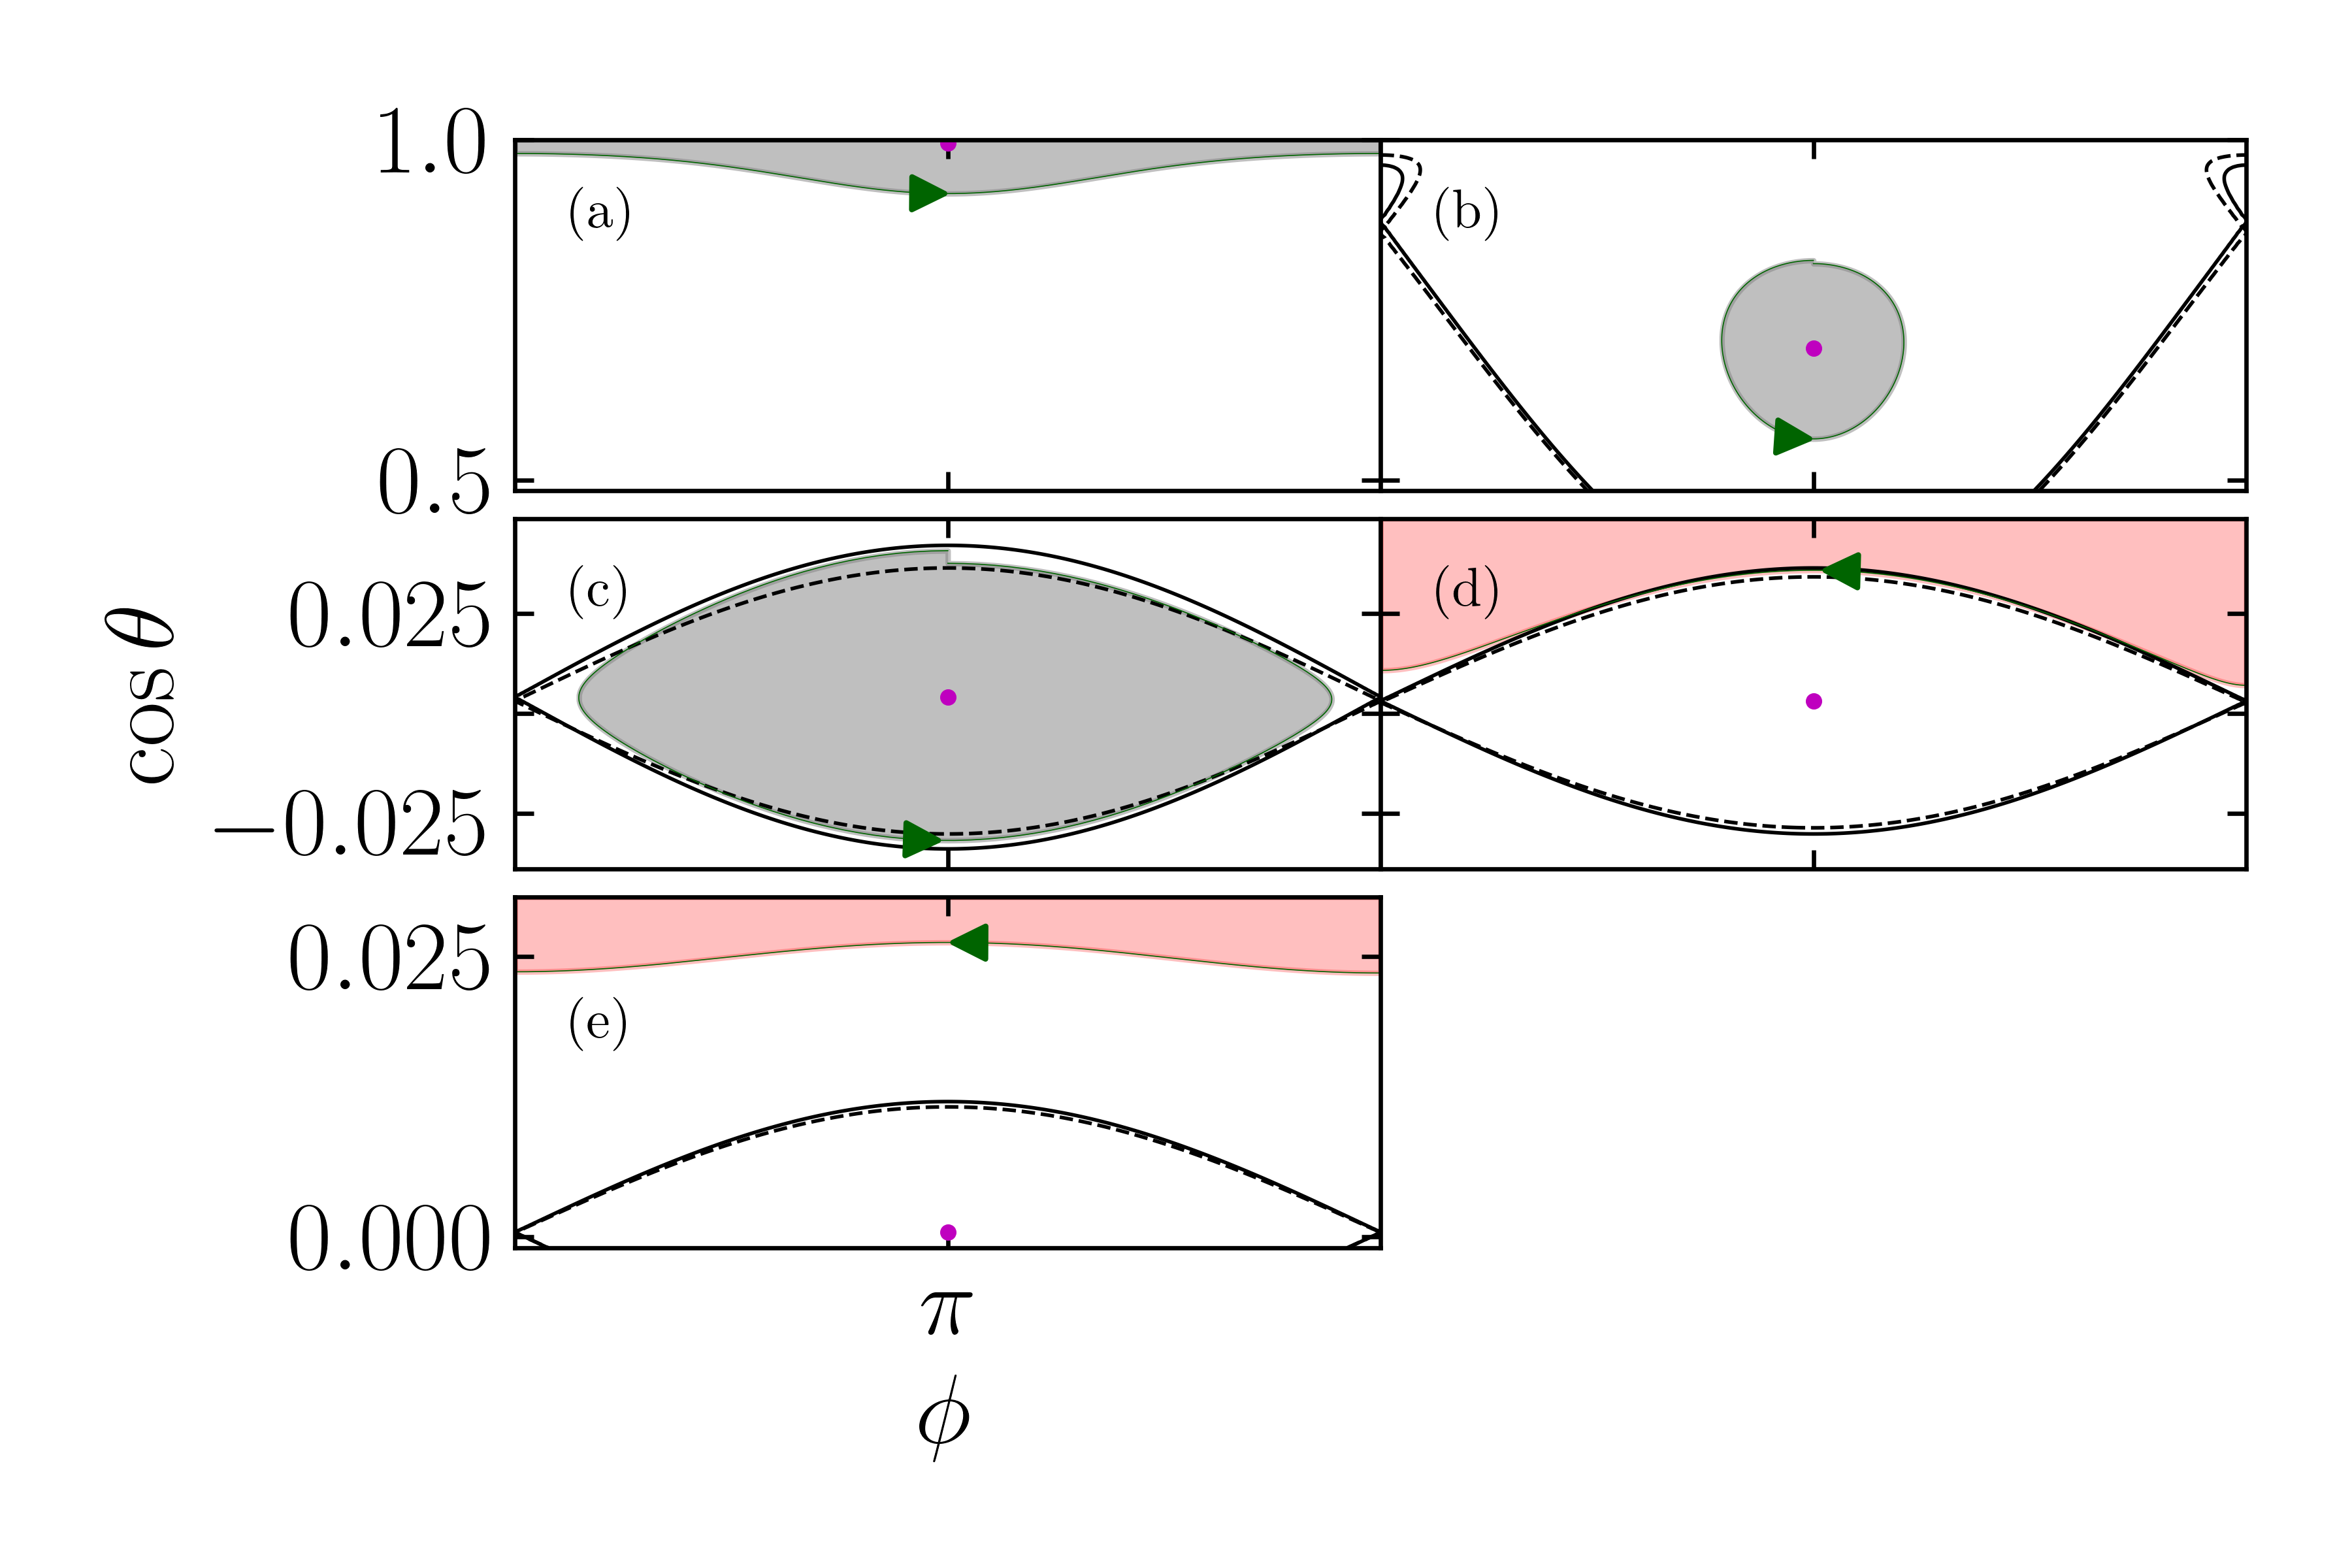
\includegraphics[width=\columnwidth]{../initial/2_toy2/3testo21_subplots.png}
    \end{subfigure}
    \caption{Fiducial simulation following the $A_{II} \to A_{I}$ transition. An
    initial $\theta_{sd, i} = 0.3\;\mathrm{rad} \approx 17.2^\circ$ was used, as
    well as $\epsilon = 3 \times 10^{-4}$. Top plot upper panel: plot of $\cos
    \theta(t)$ (green) in an example simulation. Overlaid are the locations of
    Cassini State 2 (red), and upper and lower bounds on the separatrix (black).
    Note that the trajectory successfully tracks CS2 to a misalignment angle
    $\theta \approx 90^\circ$. Light vertical blue lines denote times portrayed
    in bottom plot. Top plot lower panel: plot of the enclosed separatrix area
    obtained by integrating the simulated trajectory (blue dots) and adiabatic
    theory (red line). Lower plot: snapshots in the $\p{\cos \theta, \phi}$
    space of the simulation trajectories for the times demarcated in green
    above, corresponding to the start of the simulation, the appearance of the
    separatrix, two panels depicting the separatrix crossing process, and a
    final snapshot at $\eta = 10^{-3.5}$. The green line denotes a full
    circulation or libration cycle at the selected time, including an arrow for
    directionality. The separatrix at the start/end of the portrayed cycle are
    shown in solid/dashed black lines respectively. Also labeled is CS2 at the
    start of the cycle (red). Finally, the enclosed phase space area is shaded
    in grey ($A > 0$) and red ($A < 0$).}\label{fig:ad_21}
\end{figure}
\begin{figure}
    \centering
    \begin{subfigure}{\columnwidth}
        \centering
        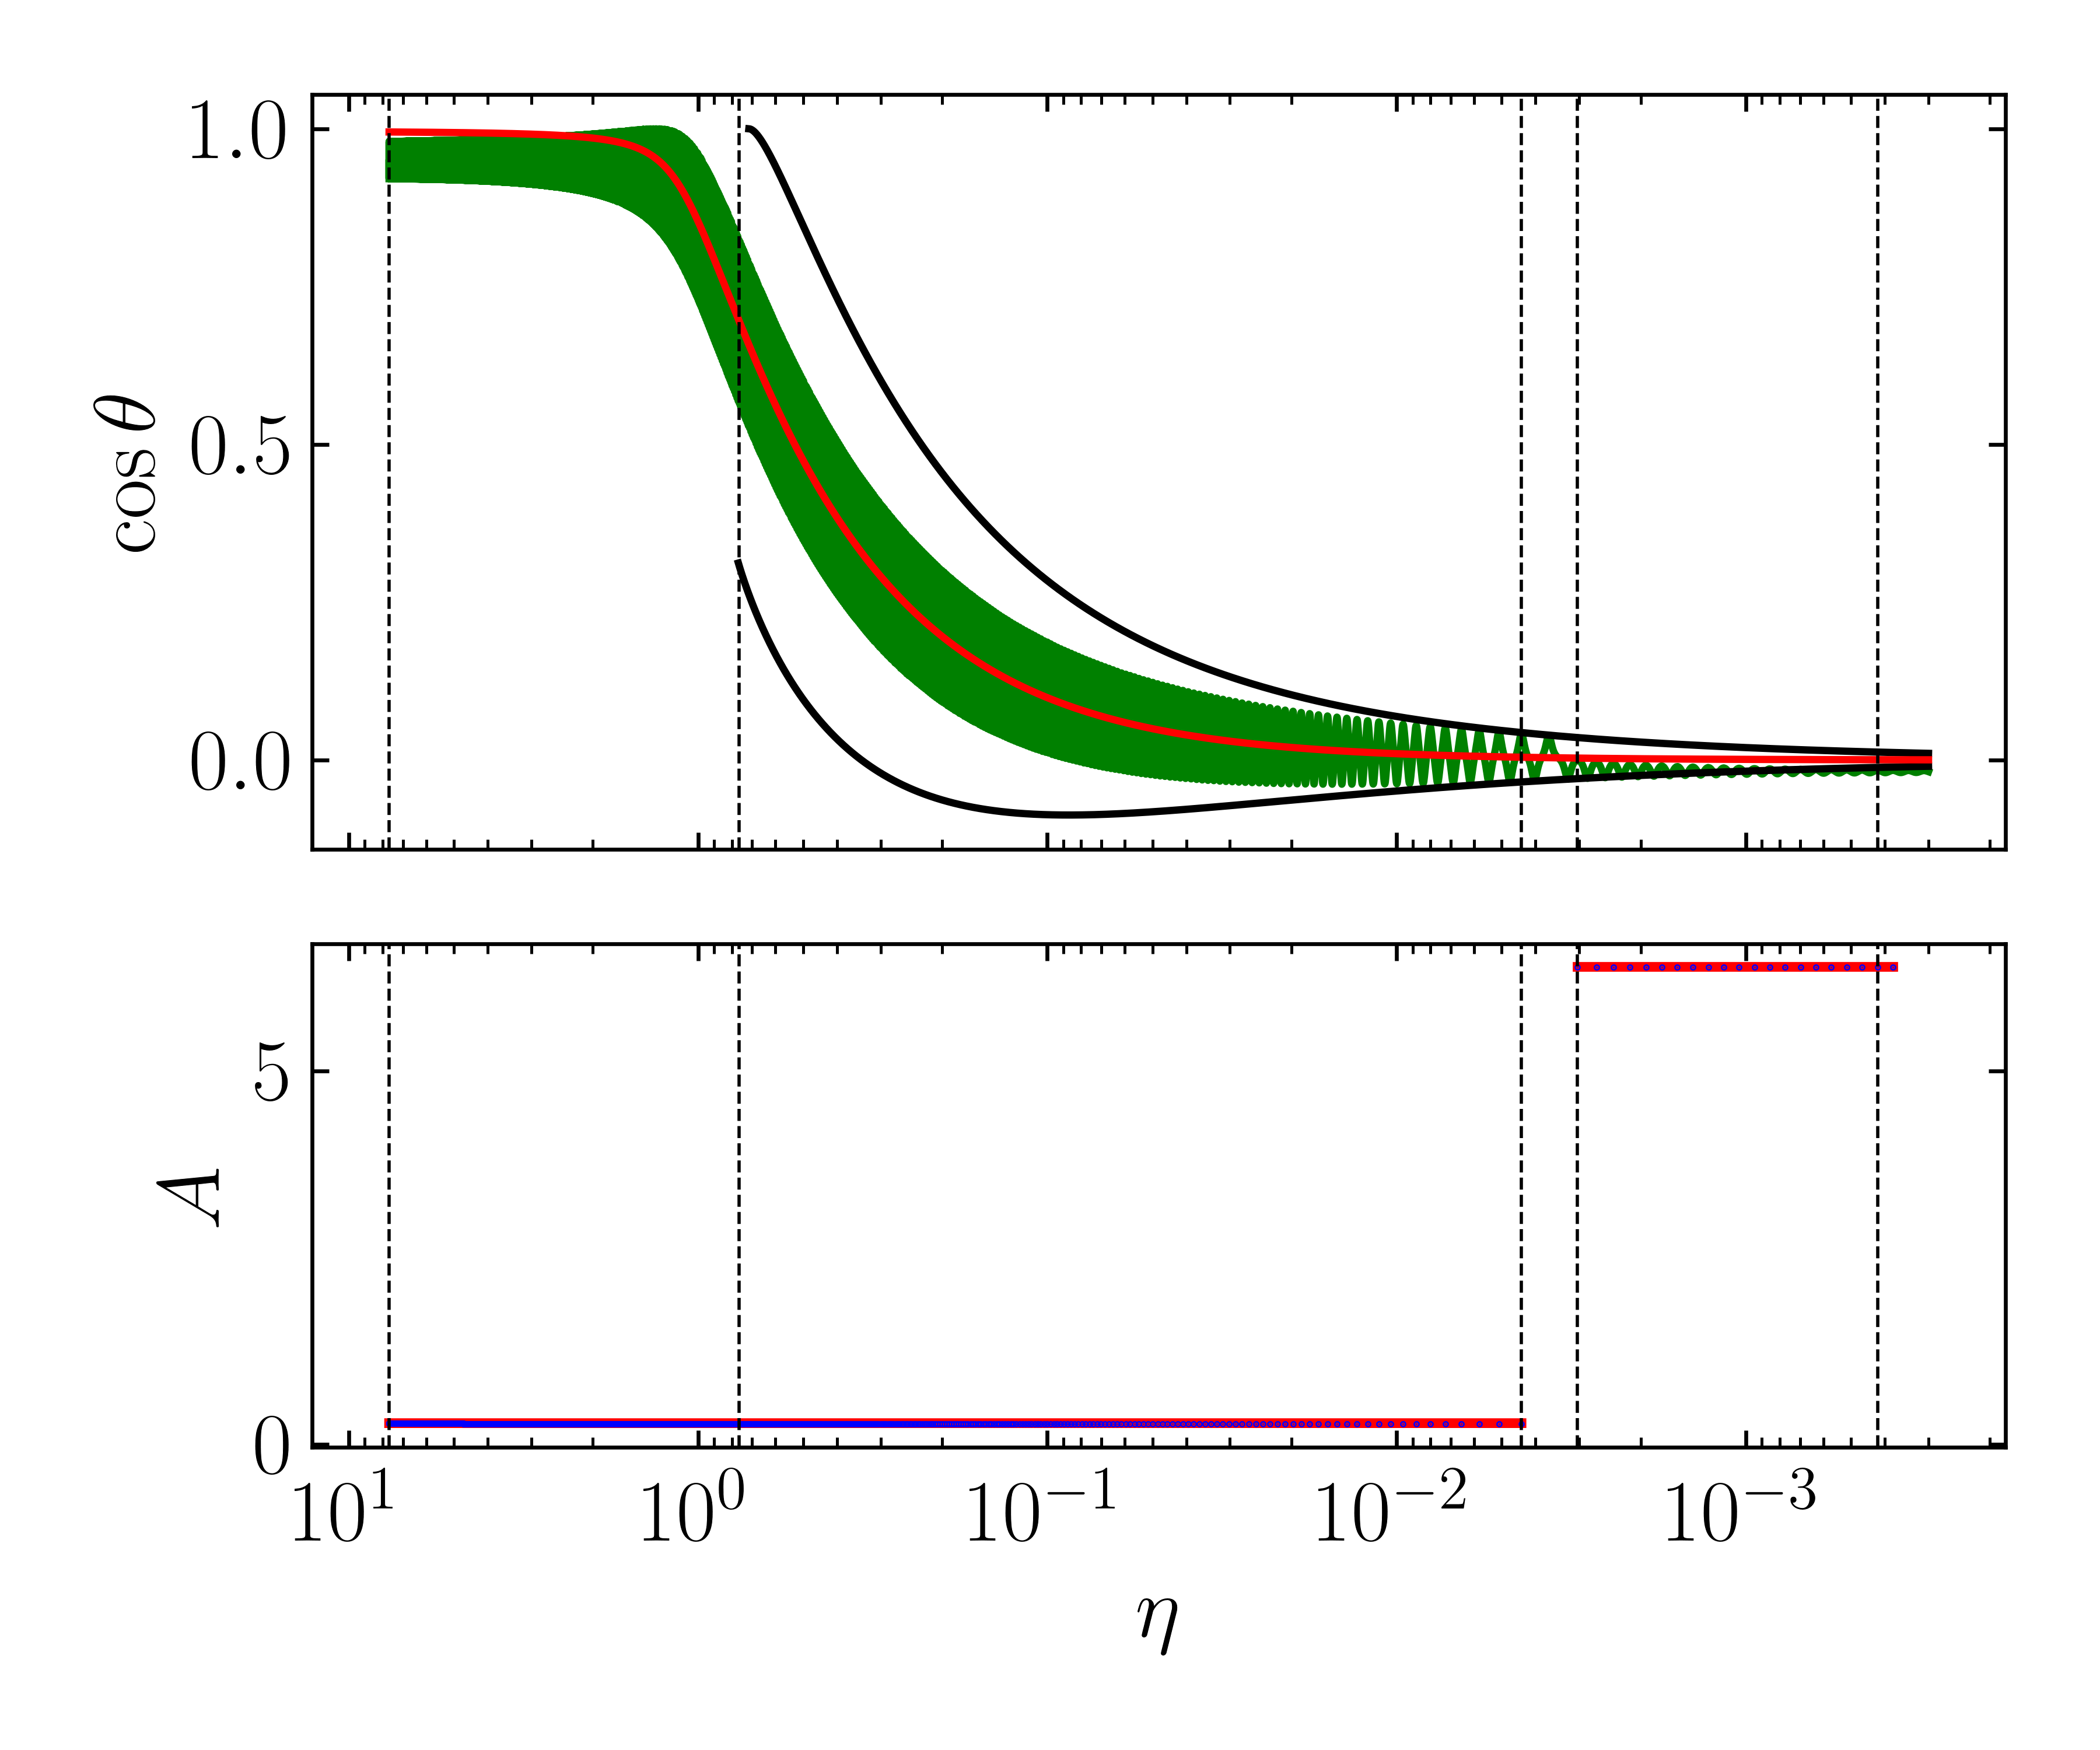
\includegraphics[width=\columnwidth]{../initial/2_toy2/3testo23.png}
    \end{subfigure}
    \begin{subfigure}{\columnwidth}
        \centering
        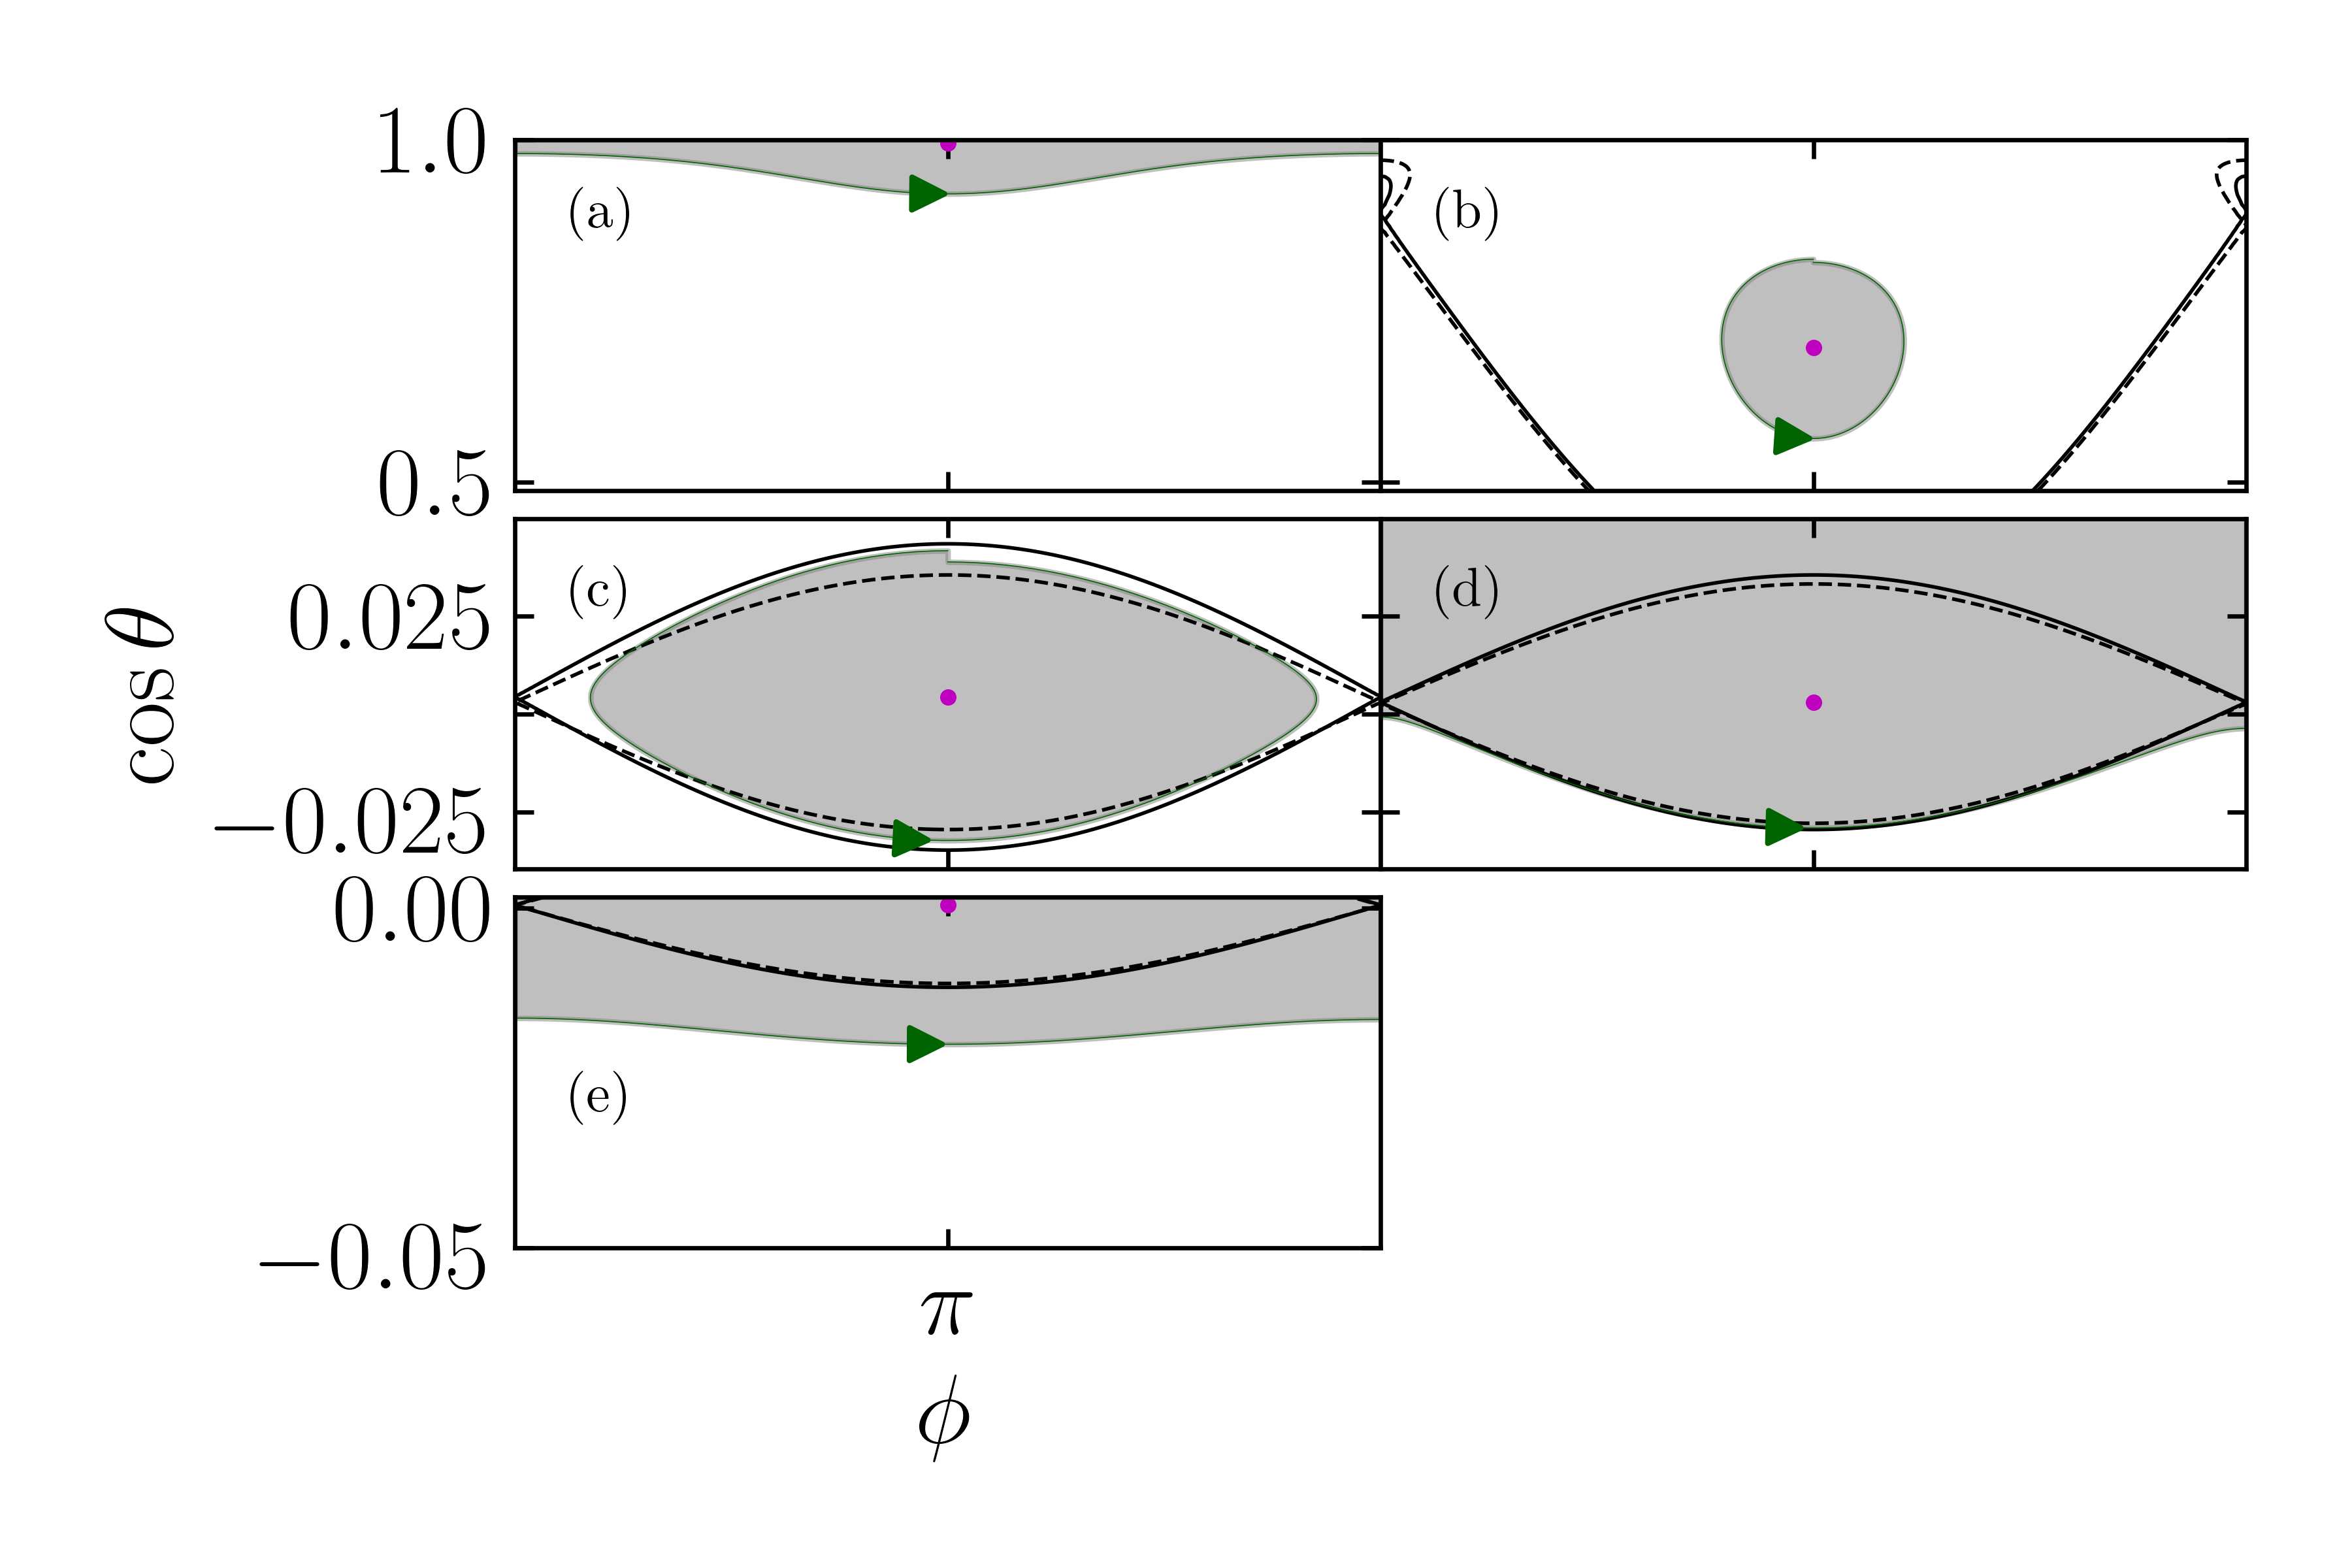
\includegraphics[width=\columnwidth]{../initial/2_toy2/3testo23_subplots.png}
    \end{subfigure}
    \caption{Same as \autoref{fig:ad_21} but for the $A_2 \to A_3$ track.
    $\theta_{sd, i} = 0.3\;\mathrm{rad}$ and $\epsilon = 3.01 \times
    10^{-4}$.}\label{fig:ad_23}
\end{figure}
\begin{figure}
    \centering
    \begin{subfigure}{\columnwidth}
        \centering
        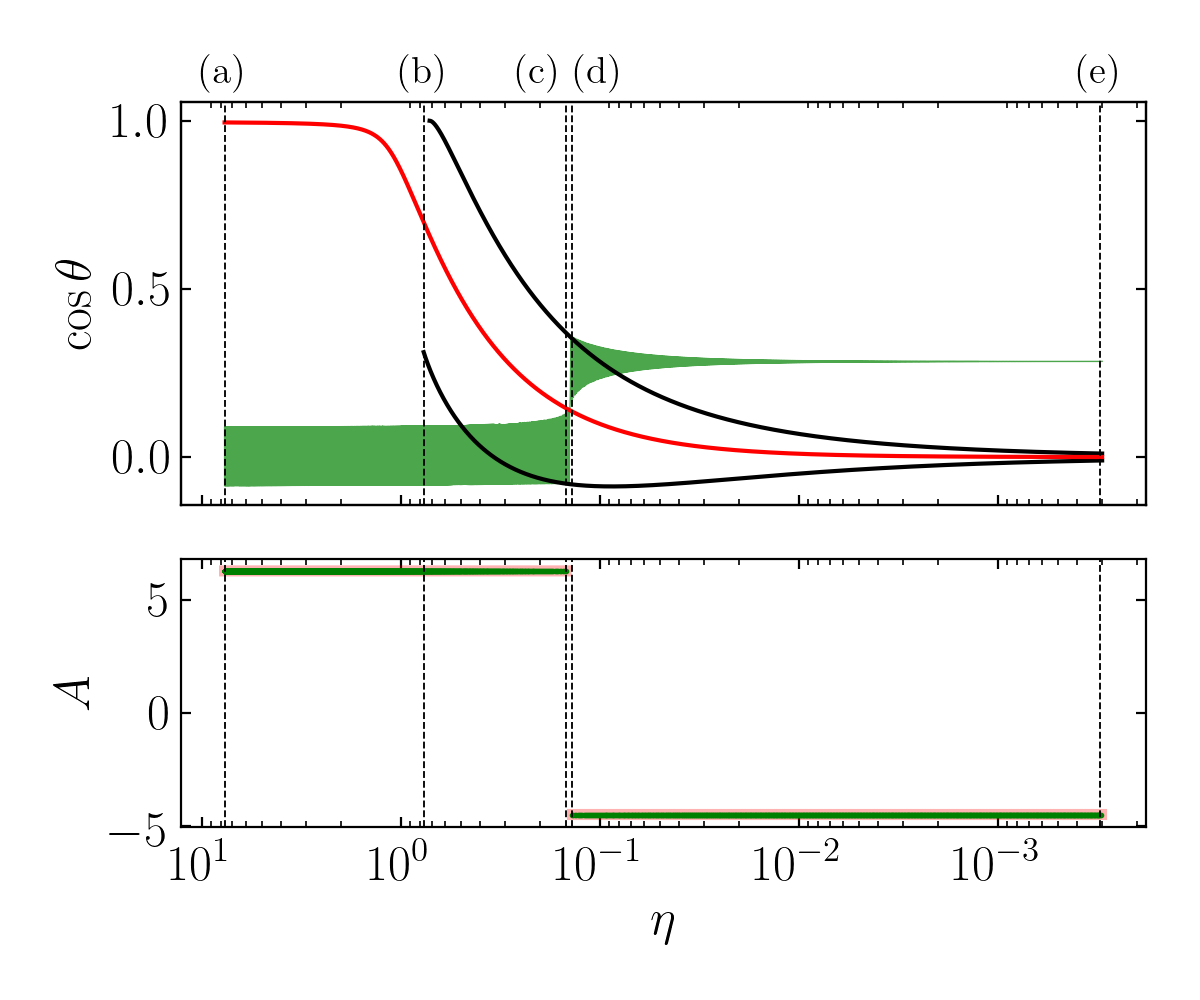
\includegraphics[width=\columnwidth]{../initial/2_toy2/3testo31.png}
    \end{subfigure}
    \begin{subfigure}{\columnwidth}
        \centering
        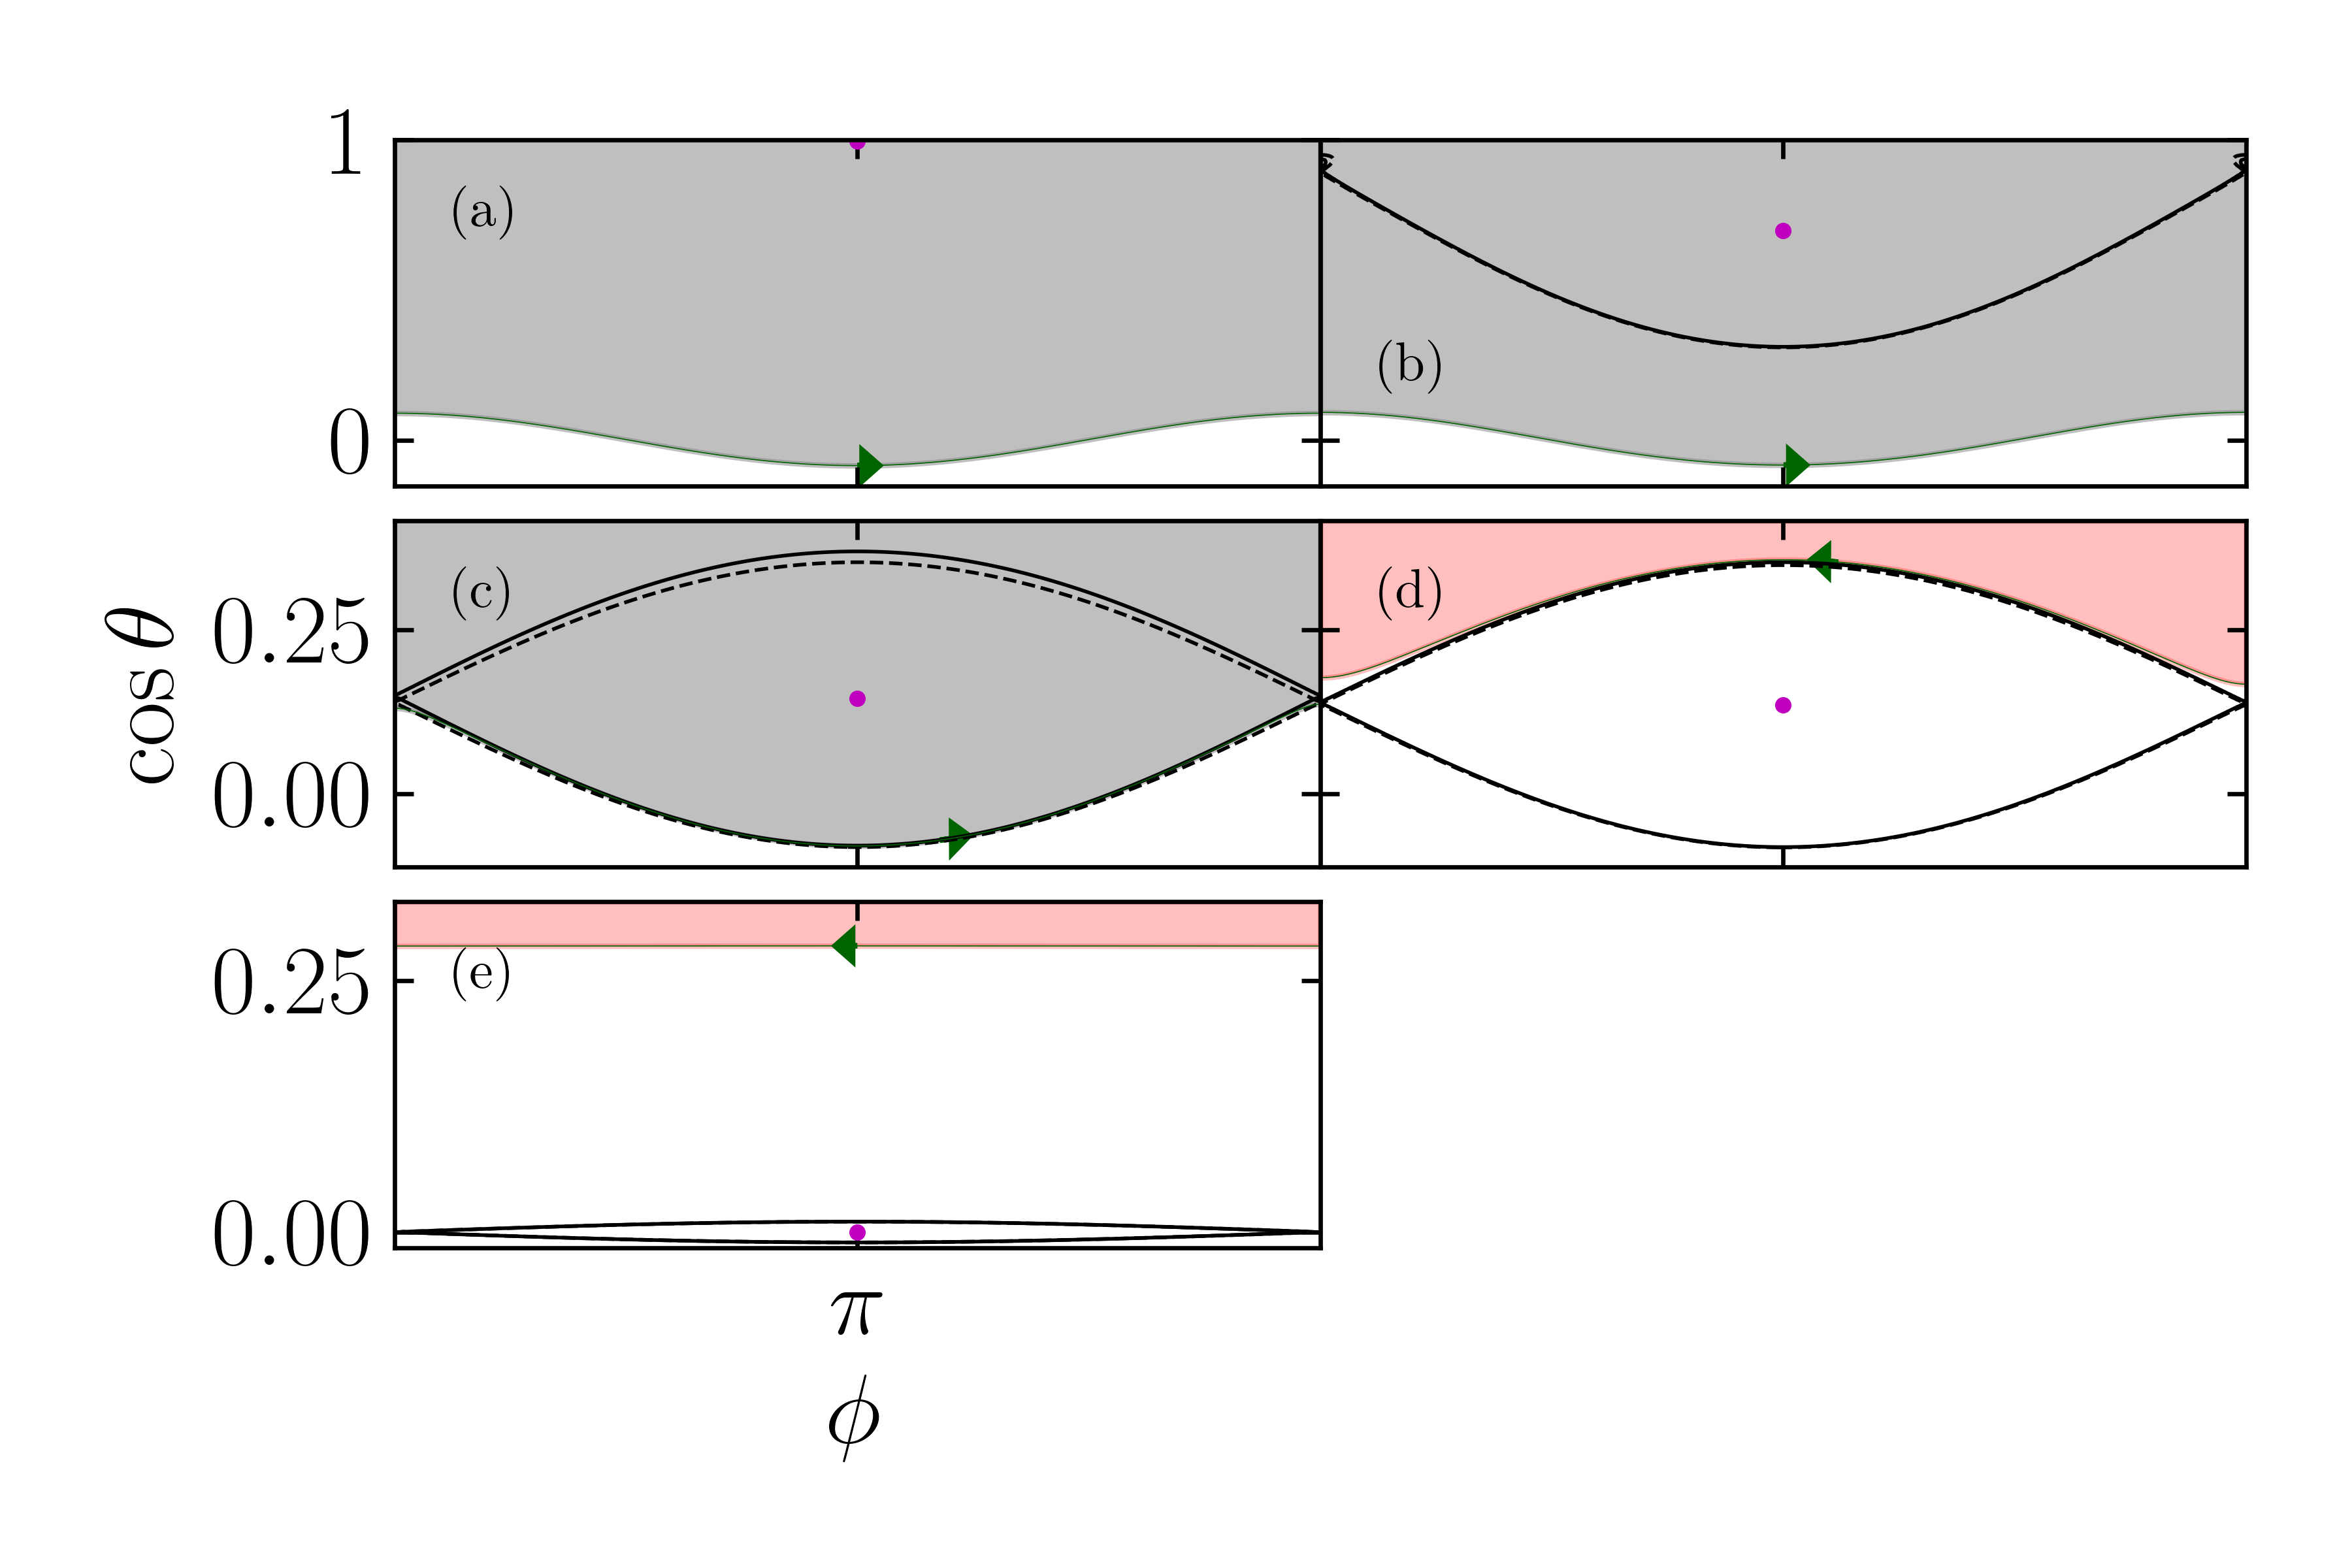
\includegraphics[width=\columnwidth]{../initial/2_toy2/3testo31_subplots.png}
    \end{subfigure}
    \caption{Same as \autoref{fig:ad_21} but for the $A_{III} \to A_I$
    track. $\theta_{sd, i} = 89.1^\circ$, and $\epsilon = 3.01 \times
    10^{-4}$.}\label{fig:ad_31}
\end{figure}
\begin{figure}
    \centering
    \begin{subfigure}{\columnwidth}
        \centering
        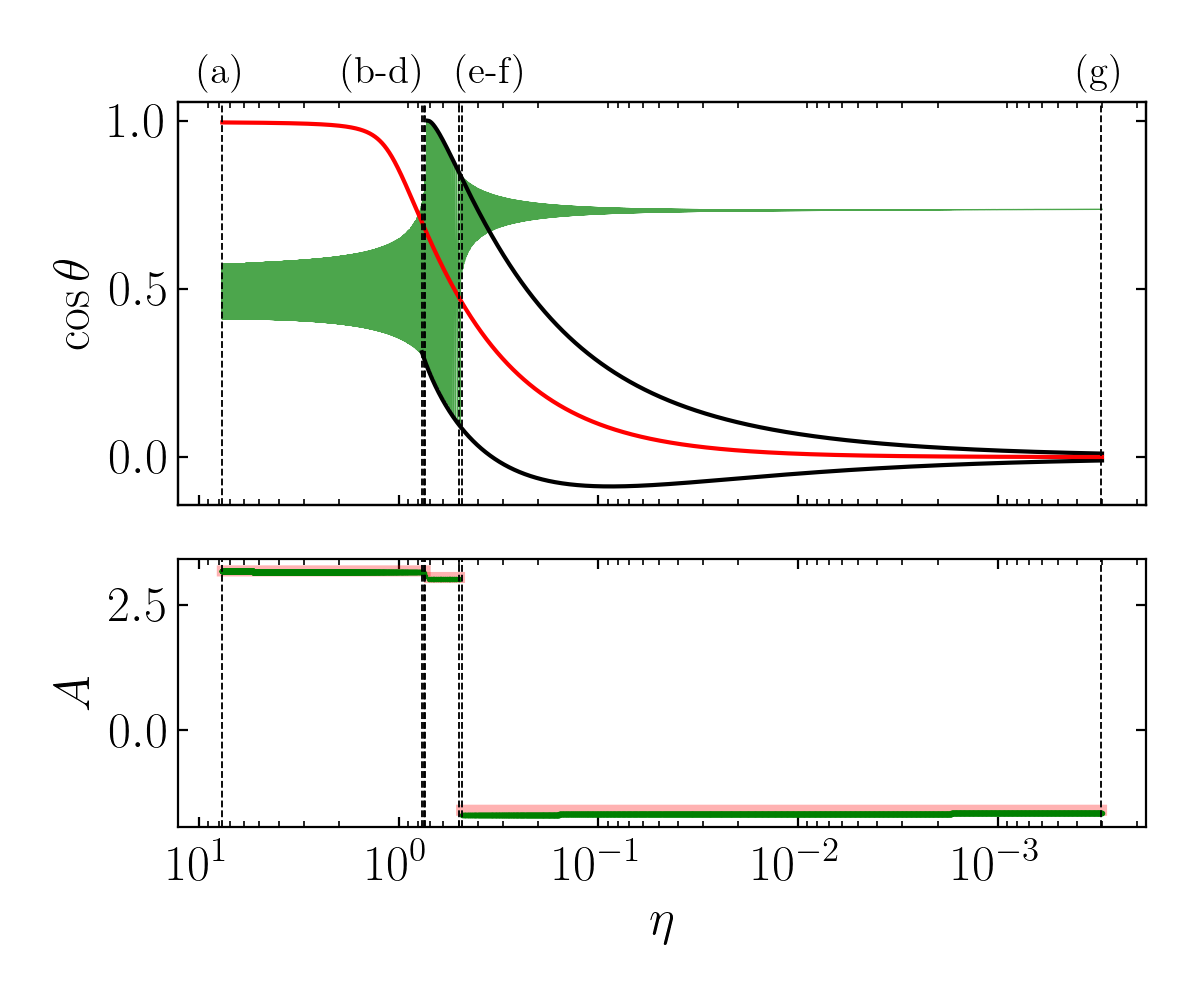
\includegraphics[width=\columnwidth]{../initial/2_toy2/3testo321.png}
    \end{subfigure}
    \begin{subfigure}{\columnwidth}
        \centering
        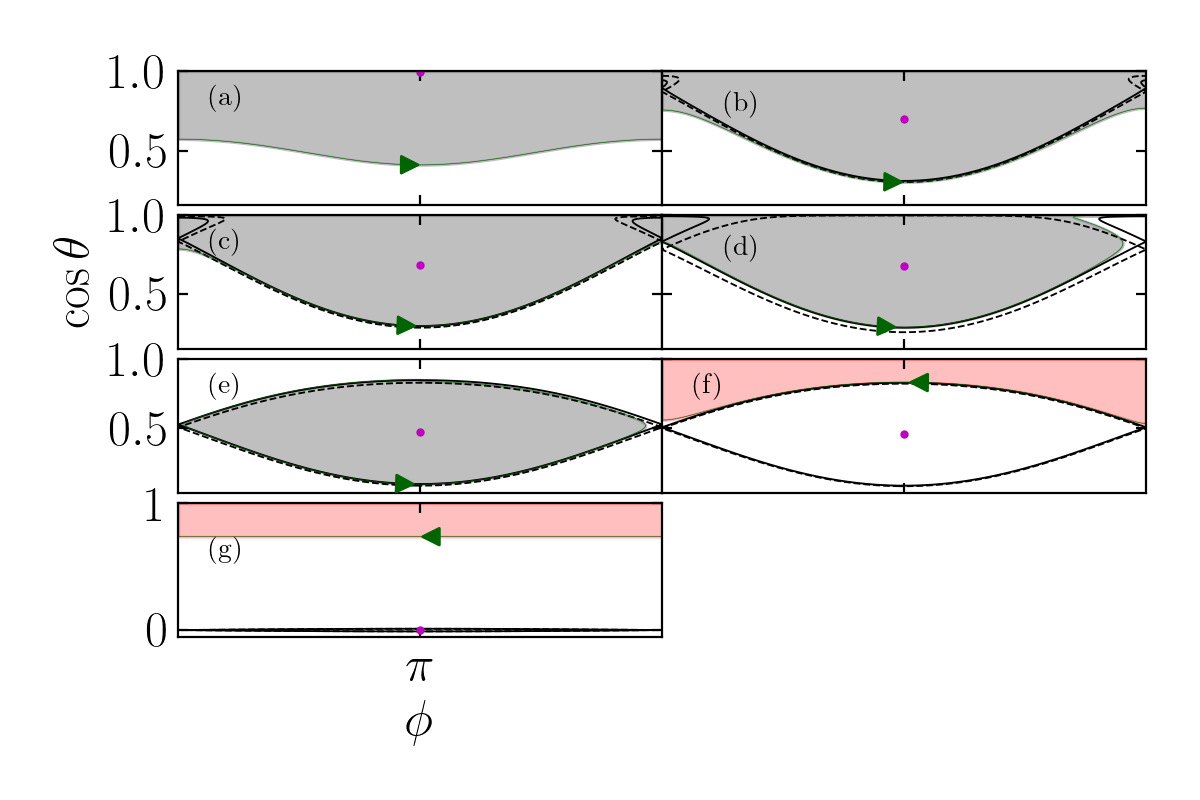
\includegraphics[width=\columnwidth]{../initial/2_toy2/3testo321_subplots.png}
    \end{subfigure}
    \caption{Same as \autoref{fig:ad_21} but for the $A_{III} \to A_{II} \to A_I$
    track. $\theta_{sd, i} = 60^\circ$, and $\epsilon = 3.14 \times 10^{-4}$.
    Two separatrix crossings are shown.}\label{fig:ad_321}
\end{figure}

\section{Nonadiabatic Effects}\label{s:nonad}

\subsection{Transition to Non-adiabaticity}

To illustrate the transition to non-adiabaticity, we present two simulations
with increasingly larger values of $\epsilon$ than \autoref{fig:ad_ensemble}
below in \autoref{fig:3_ensemble_05_25} and \autoref{fig:3_ensemble_05_15}.

At first non-adiabaticity manifests as a larger scatter of final obliquities
near the tracks predicted from adiabatic evolution. These scatters first set in
for trajectories starting in zone $III$, as these cross the separatrix at higher
values of $\theta$ and have a stricter adiabaticity criterion (see
\autoref{eq:ad_constr}).

Later, these large scatters take on band-like structures that seem to persist
across values of $\theta_{sd, i}$; we attribute these to the separatrix crossing
process becoming sensitive to the \emph{phase} of the final
libration/circulation orbit at separatrix crossing. This is equivalent to
separatrix crossing no longer being significantly slower than the resonant
libration period and violating the adiabatic assumption.
\begin{figure}
    \centering
    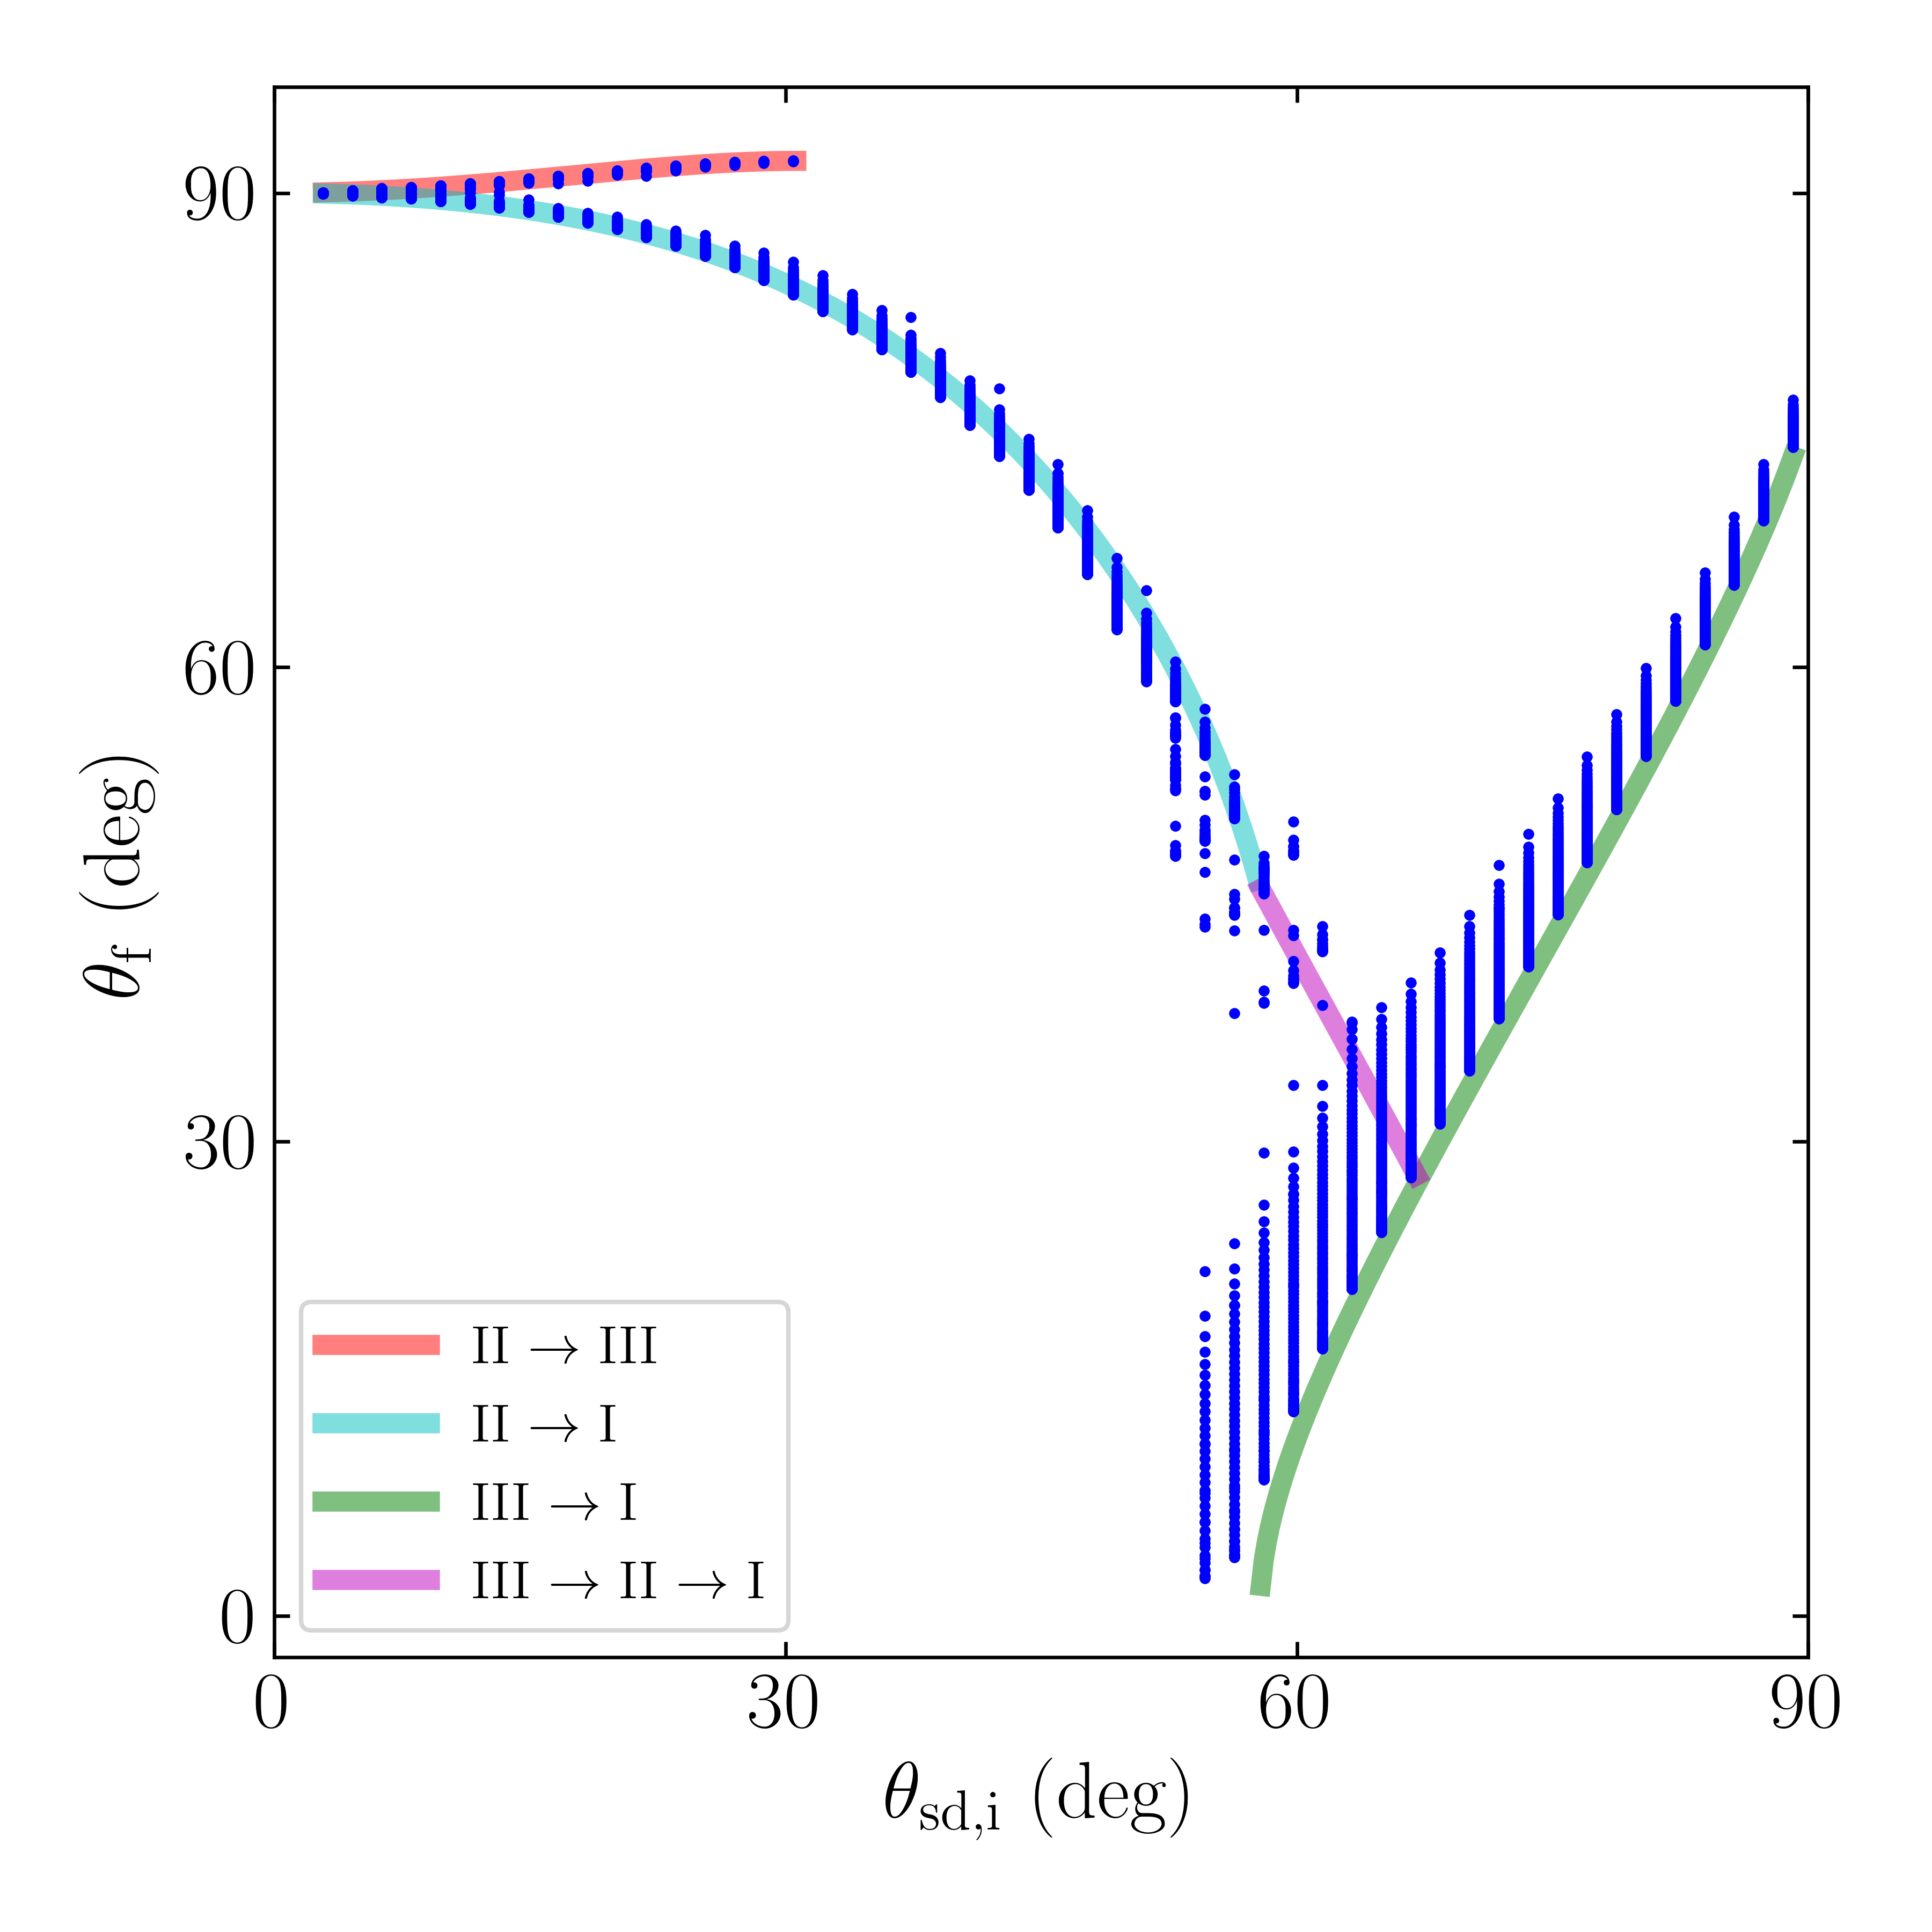
\includegraphics[width=\columnwidth]{../initial/2_toy2/3_ensemble_05_25.png}
    \caption{Same as \autoref{fig:ad_ensemble} but for $\epsilon = 10^{-2.5}$,
    and restricting $\theta_{sd, i} < 90^\circ$. A larger spread from the
    dynamical tracks is observed in the data.}\label{fig:3_ensemble_05_25}
\end{figure}
\begin{figure}
    \centering
    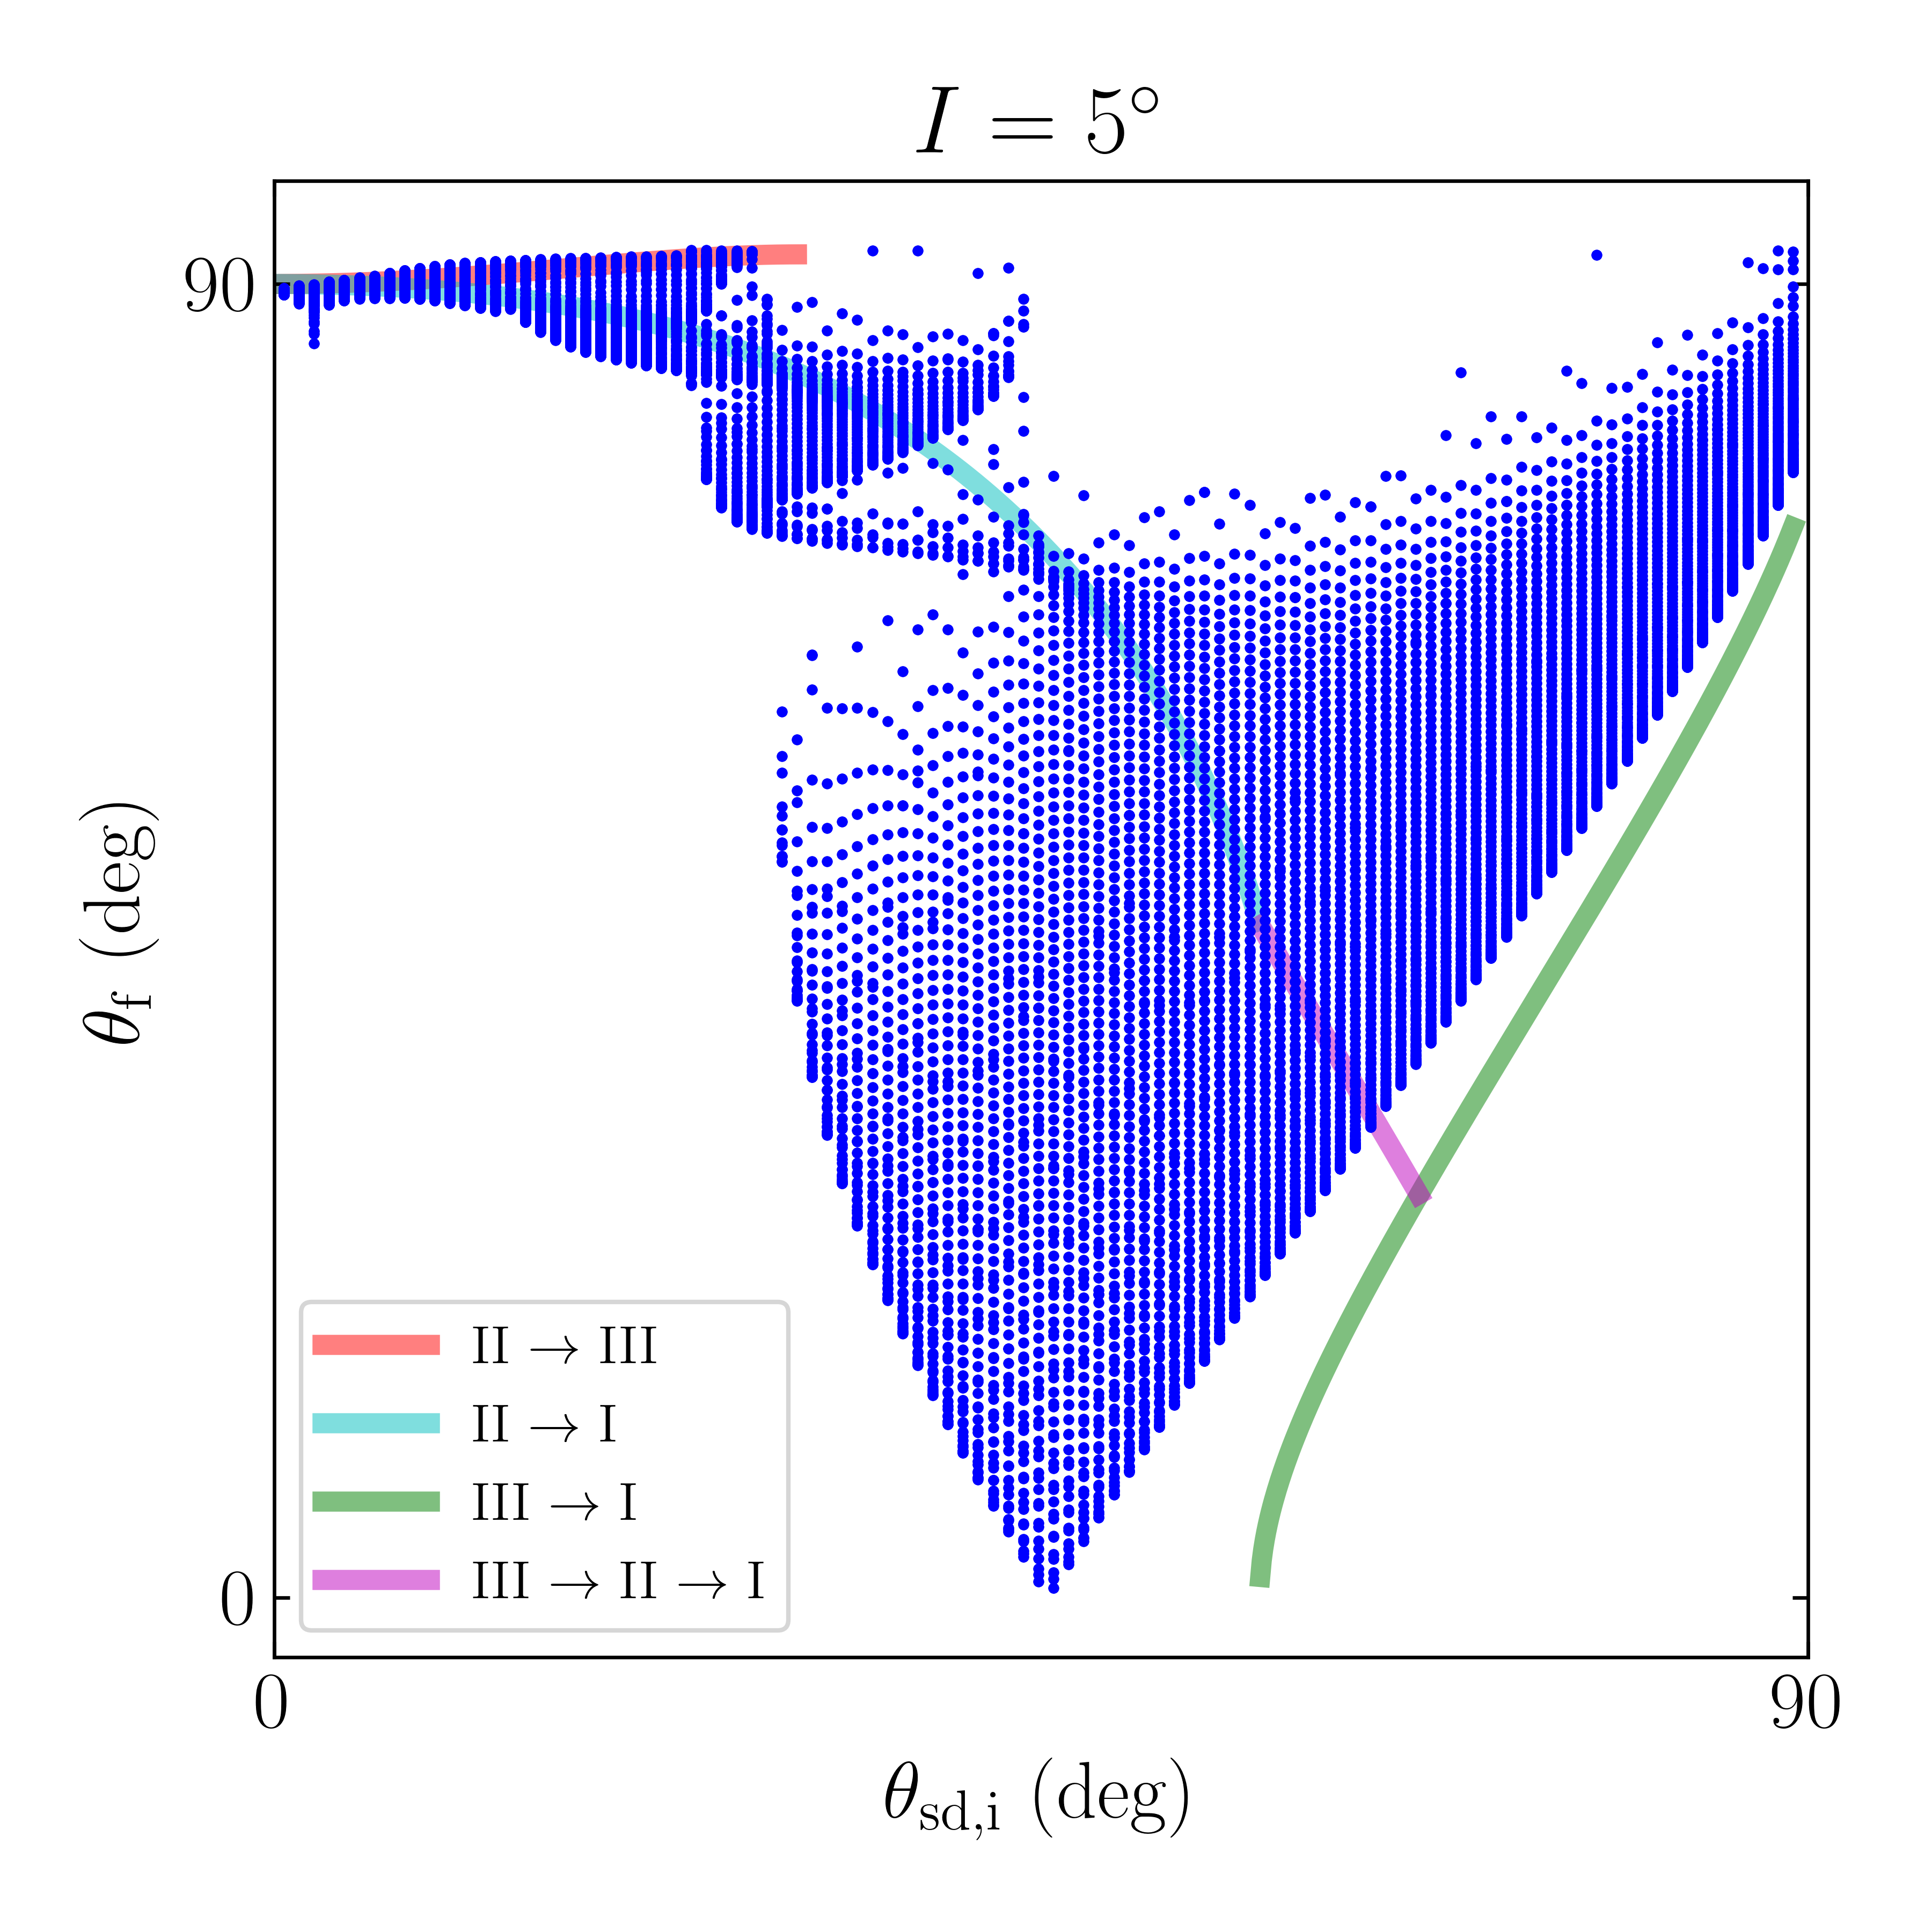
\includegraphics[width=\columnwidth]{../initial/2_toy2/3_ensemble_05_15.png}
    \caption{Same as \autoref{fig:3_ensemble_05_25} but for $\epsilon =
    10^{-1.5}$. Some small semblance of the evolutionary tracks remains, and the
    deviations appear to have a banded structure. This can be attributed to
    non-adiabaticity ``freezing-in'' the phase of the obliquity variations over
    the final libration/circulation orbit prior to separatrix
    crossing.}\label{fig:3_ensemble_05_15}
\end{figure}

A sample trajectory following in the style of \autoref{fig:ad_21} but for
$\epsilon = 0.3$ is provided in \autoref{fig:nonad_traj}. It is clear the
trajectory does not track level curves of the Hamiltonian during each individual
snapshot (e.g.\ the third snapshot).
\begin{figure}
    \centering
    \begin{subfigure}{\columnwidth}
        \centering
        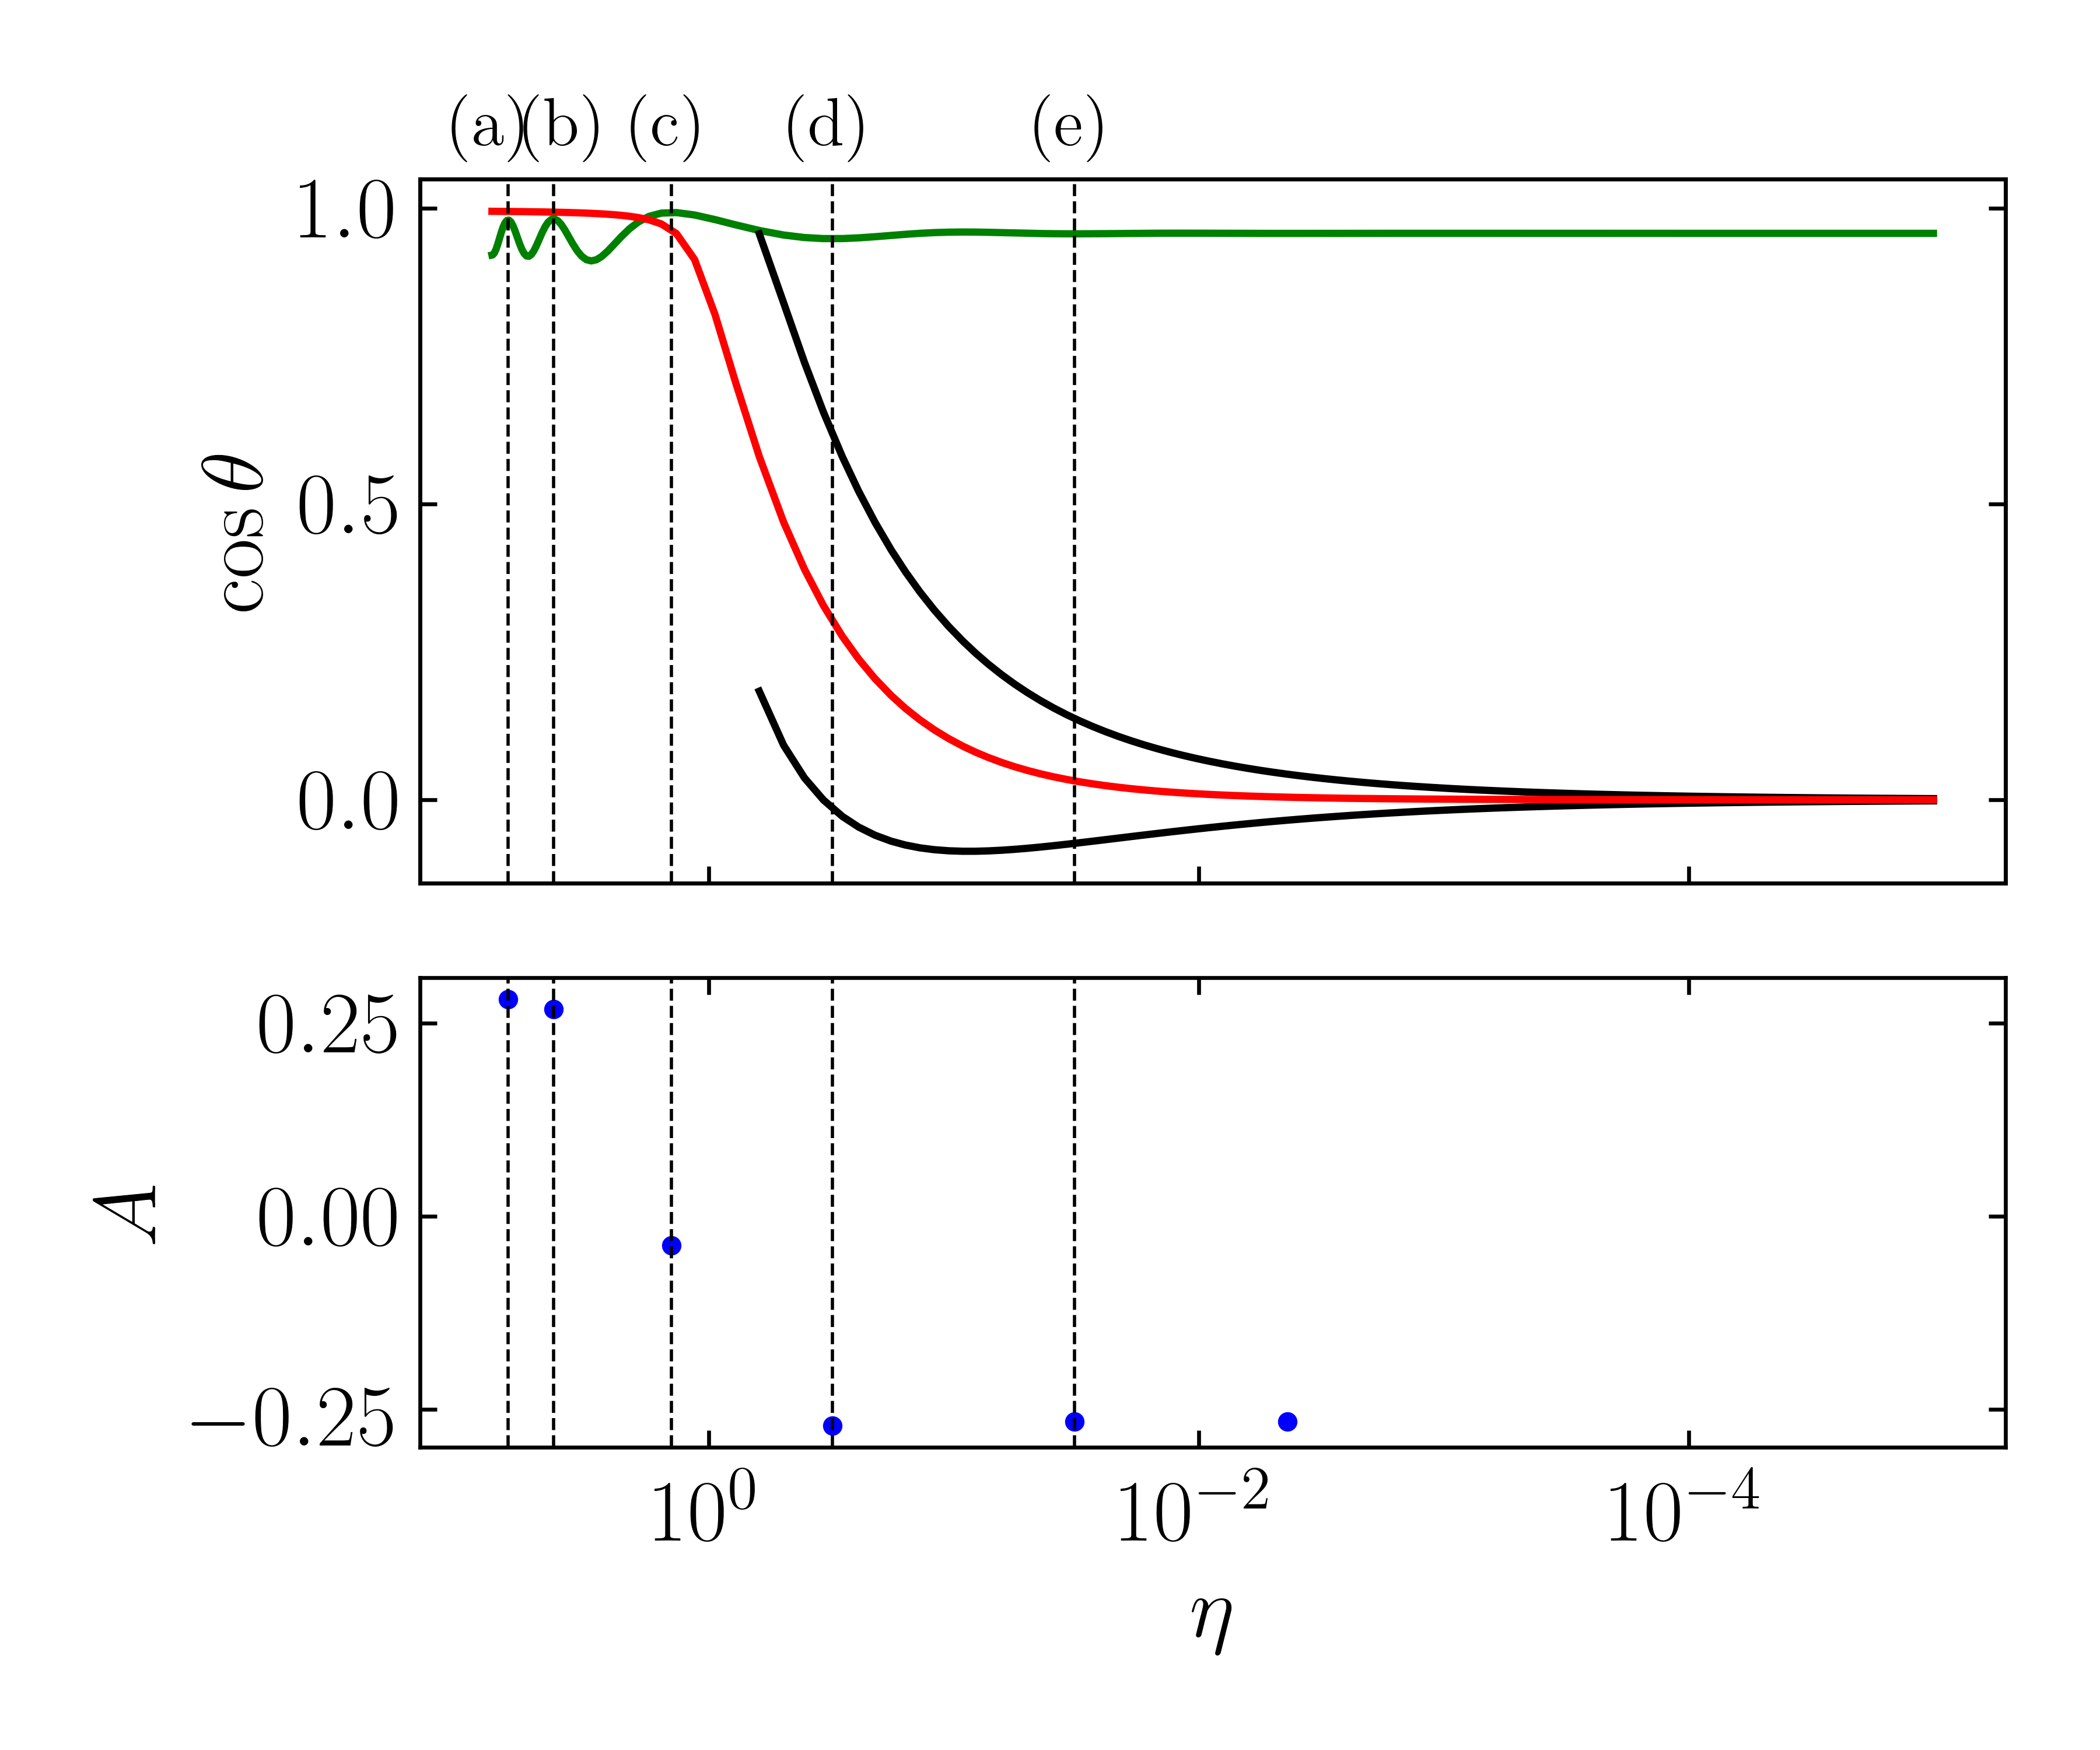
\includegraphics[width=\columnwidth]{../initial/2_toy2/3testo_nonad.png}
    \end{subfigure}
    \begin{subfigure}{\columnwidth}
        \centering
        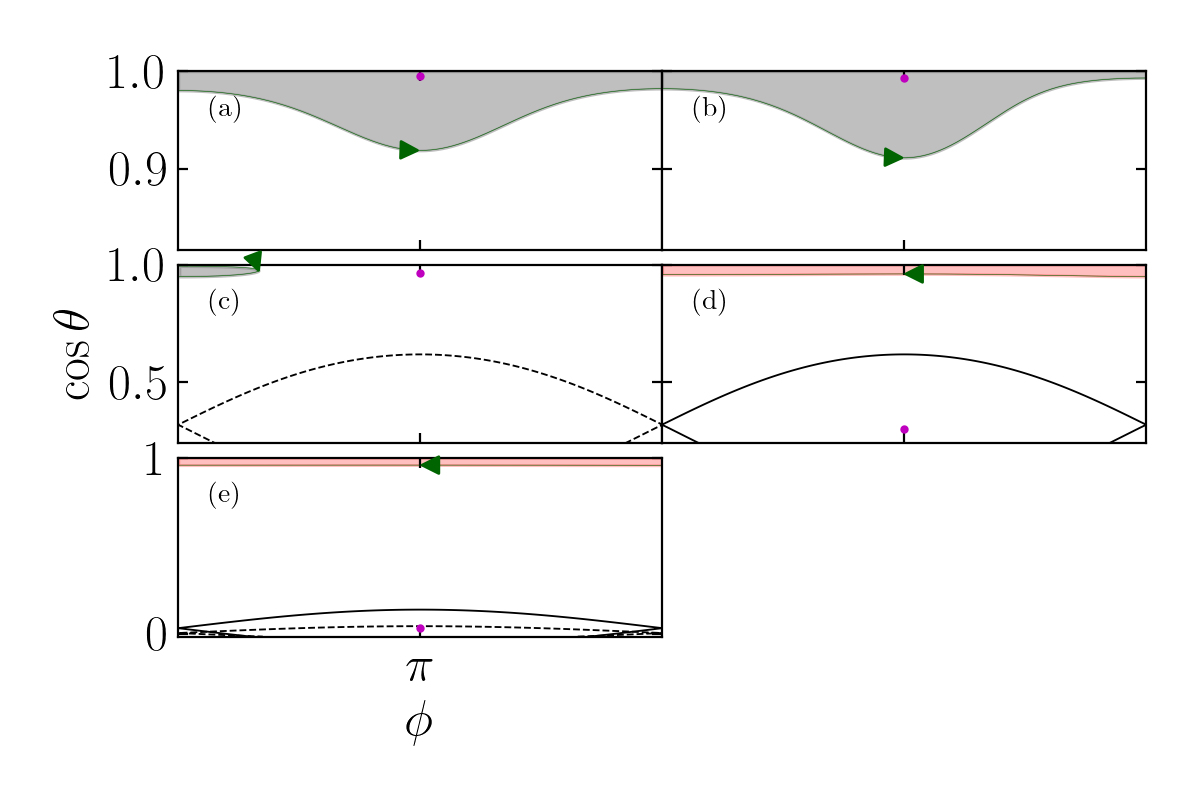
\includegraphics[width=\columnwidth]{../initial/2_toy2/3testo_nonad_subplots.png}
    \end{subfigure}
    \caption{Same as \autoref{fig:ad_21} but for a non-adiabatic $\epsilon =
    0.3$. In the top panel of the top plot, it is evident that the libration
    cycle about CS2 is unable to keep up with the swift motion of CS2 as $\eta$
    changes, decreasing the obliquity jump. In the bottom plot, we can see that
    individual orbits do not lie along level curves of the Hamiltonian, a
    further consequence of violating adiabaticity.}\label{fig:nonad_traj}
\end{figure}

\subsection{Non-adiabatic Evolution Outcomes}

A formula for $\theta_{f}$ assuming $\theta_{sd, i} = 0$ initially can be
given (see \autoref{s:app_transition})
\begin{equation}
    \theta_{f}\p{\theta_{sd, i} = 0} = \sqrt{\frac{2\pi}{\epsilon}}
        \tan I\cos I.\label{eq:nonad_q_f}
\end{equation}
We can naively generalize this by recognizing that any nonzero $\theta_{sd, i}$
manifests as obliquity variations as $\hat{s}$ librates about $\hat{l}_d$. These
can be accounted for by simply allowing the final obliquity to vary over the
same range as the initial obliquity, or,
\begin{equation}
    \theta_{f}\p{\theta_{sd, i}} - \sqrt{\frac{2\pi}{\epsilon}}
        \tan I\cos I\in \s{-\theta_{sd, i}, \theta_{sd,i}}
        .\label{eq:nonad_q_f_dist}
\end{equation}

We present the results of simulations for using $\epsilon = 0.3$ in
\autoref{fig:nonad_3_ensemeble}.
\begin{figure}
    \centering
    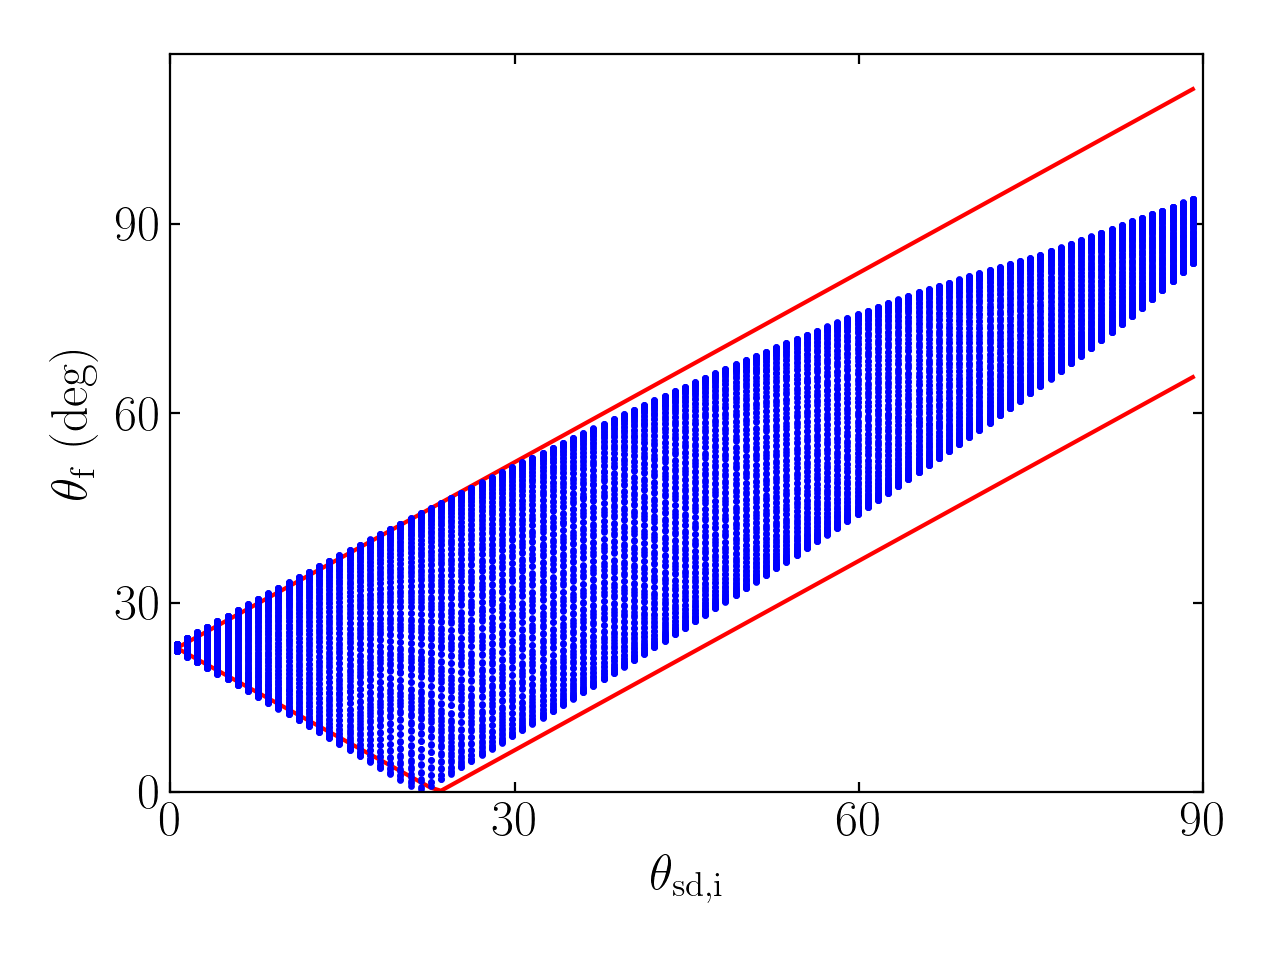
\includegraphics[width=\columnwidth]{../initial/2_toy2/3_ensemble_05_05.png}
    \caption{$\theta_{ f}\p{\theta_{sd, i}}$ at $\epsilon = 0.3$, firmly in
    the non-adiabatic regime. Note the clear double-valuedeness has disappeared,
    as have distinct dynamical tracks. The red dotted line presents the
    analytical prediction given by
    \autoref{eq:nonad_q_f_dist}.}\label{fig:nonad_3_ensemeble}
\end{figure}

The agreement of \autoref{eq:nonad_q_f} at fixed $I$ for varying $\epsilon$ is
shown in \autoref{fig:nonad_3_scan}. Note that $\epsilon \to 0$ recovers the
adiabatic regime. The deviation of $\theta_f$ from the analytical prediction
within the adiabatic regime is indeed due to adiabatic effects becoming
dominant; compare to \autoref{fig:nonad_3_scan_20} where little deviation is
observed until $\theta_f \approx 90^\circ$.
\begin{figure}
    \centering
    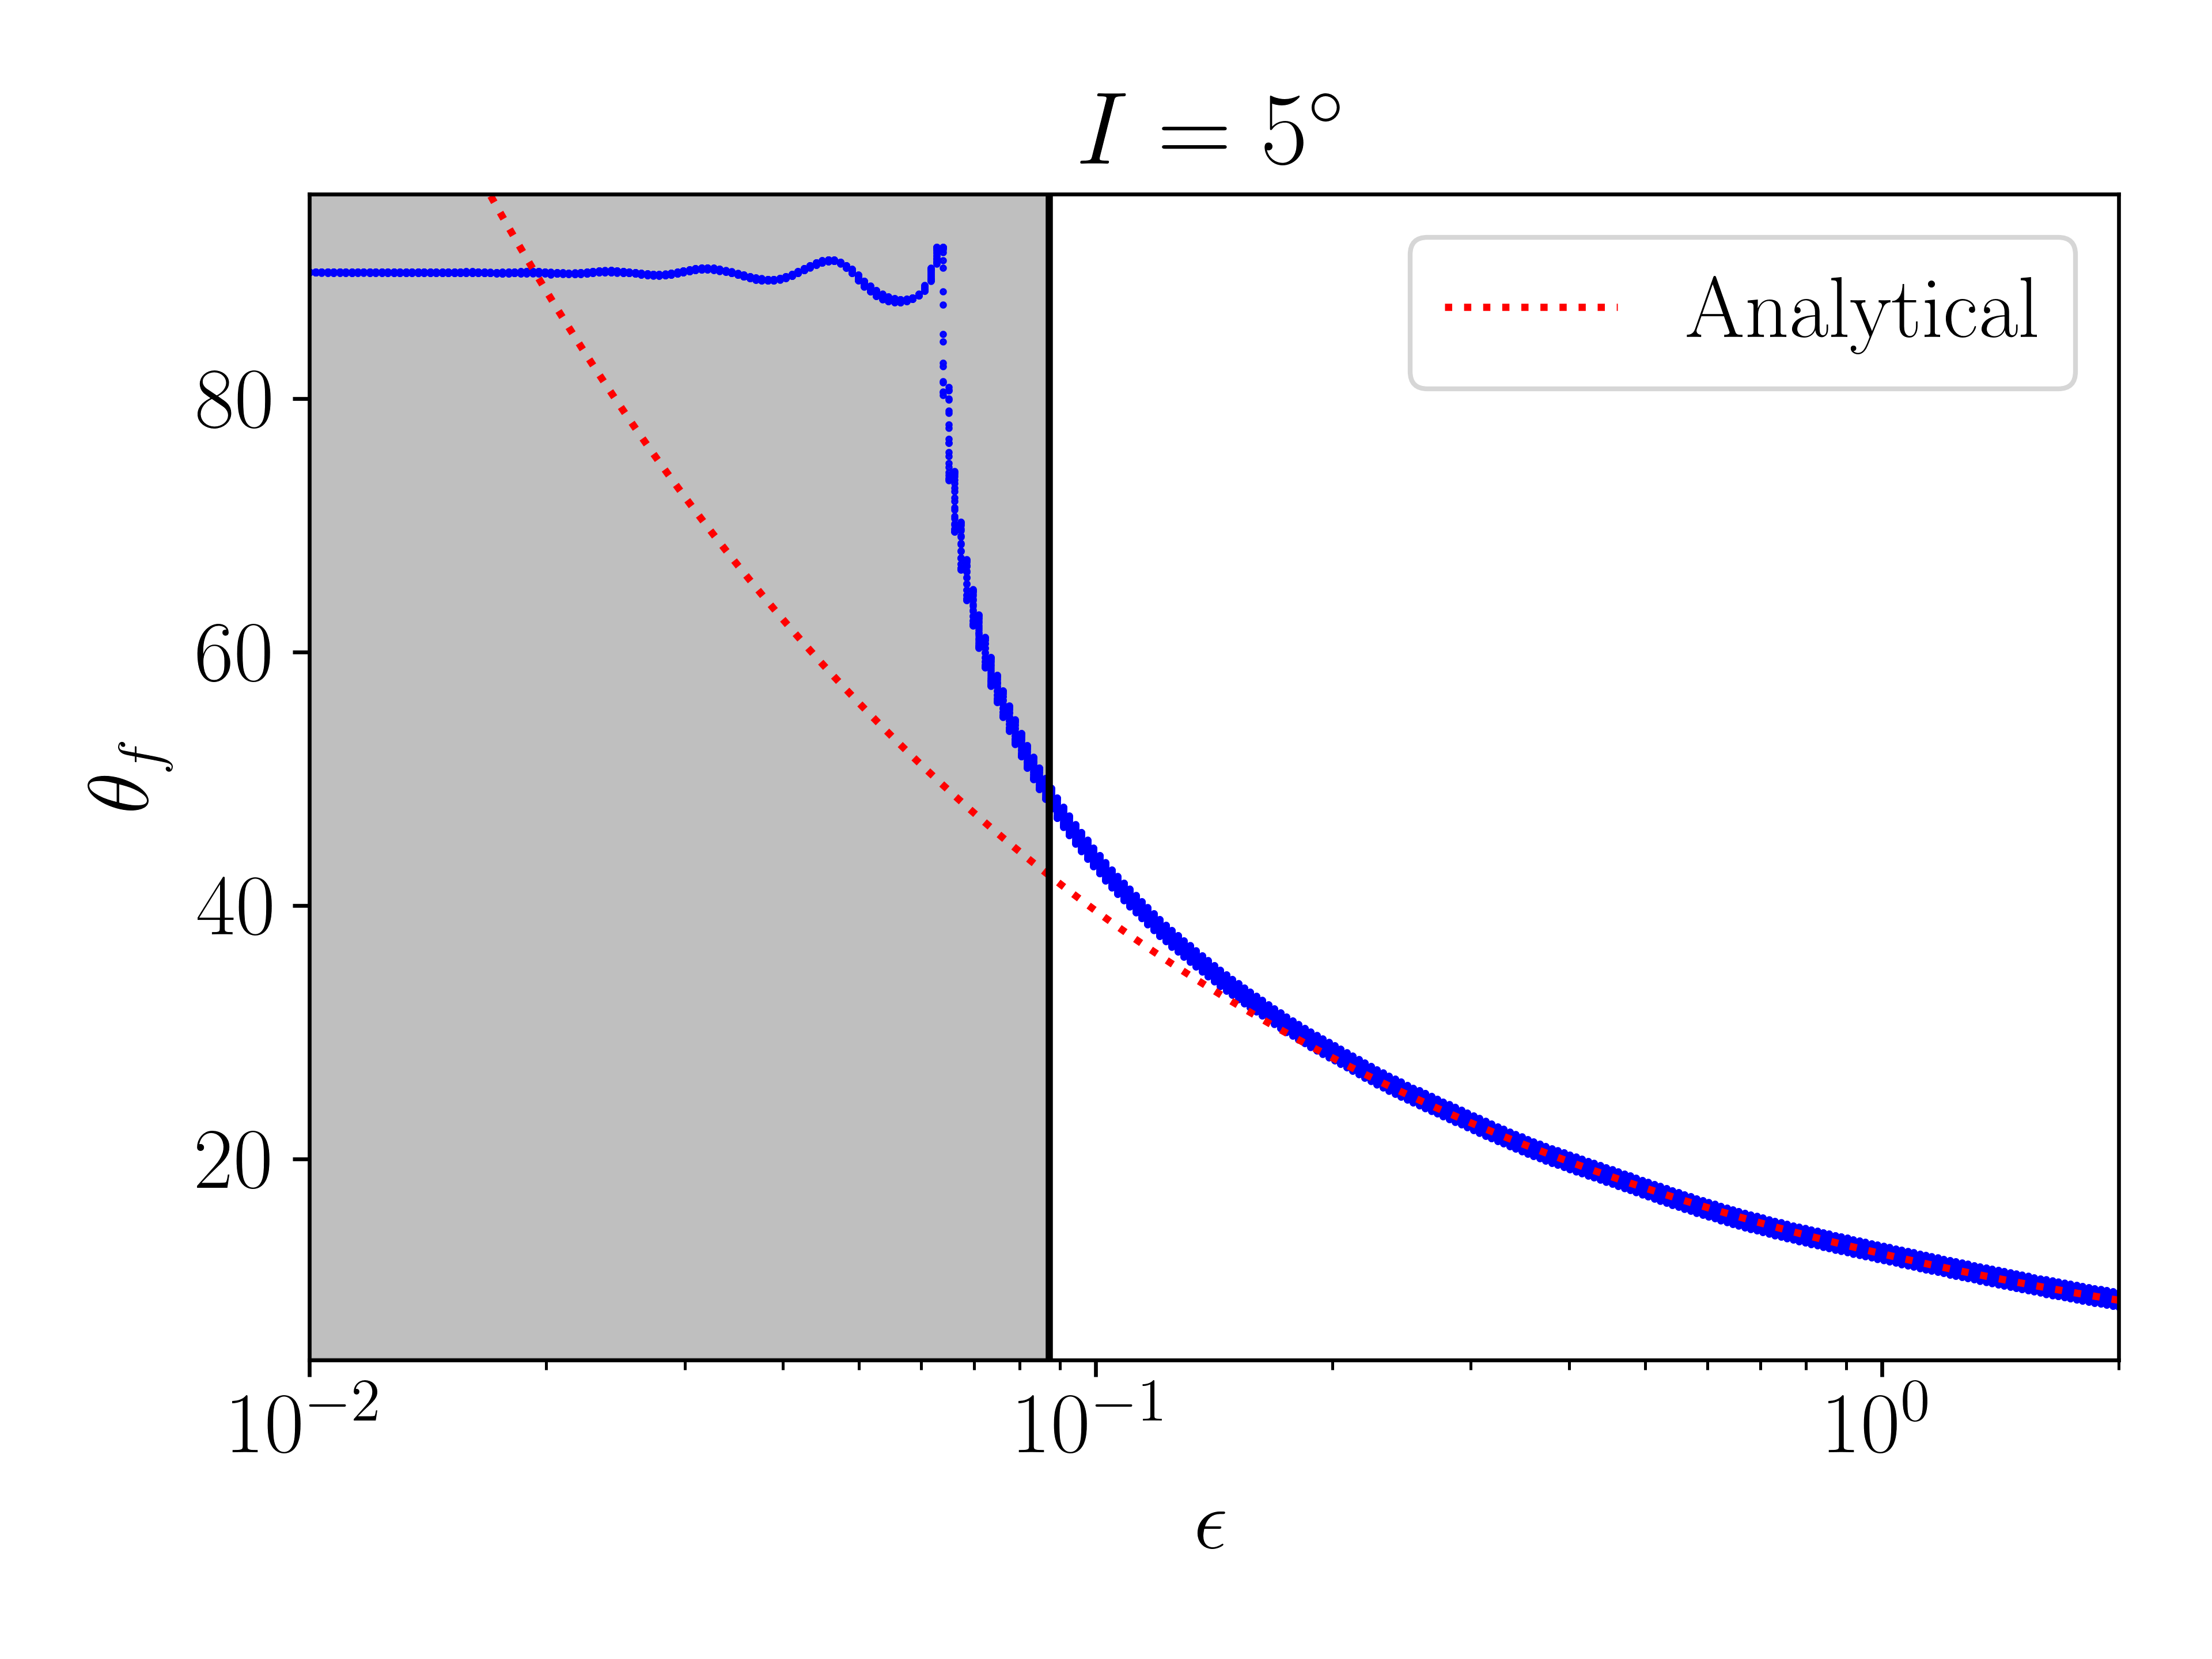
\includegraphics[width=\columnwidth]{../initial/2_toy2/3scan.png}
    \caption{Plot of $\theta_{ f}\p{\theta_{sd, i} = 0}$ as a function of
    $\epsilon$, where $I = 5^\circ$. The shaded area, bordered by the black
    line, corresponds to the adiabatic regime estimated by
    \autoref{eq:ad_constr}. Overplotted in the red line is
    \autoref{eq:nonad_q_f}, which is in good agreement for $\epsilon \gtrsim
    0.1$ the non-adiabatic regime, while $\theta_{f} \approx 90^\circ$ in the
    adiabatic regime.}\label{fig:nonad_3_scan}
\end{figure}
\begin{figure}
    \centering
    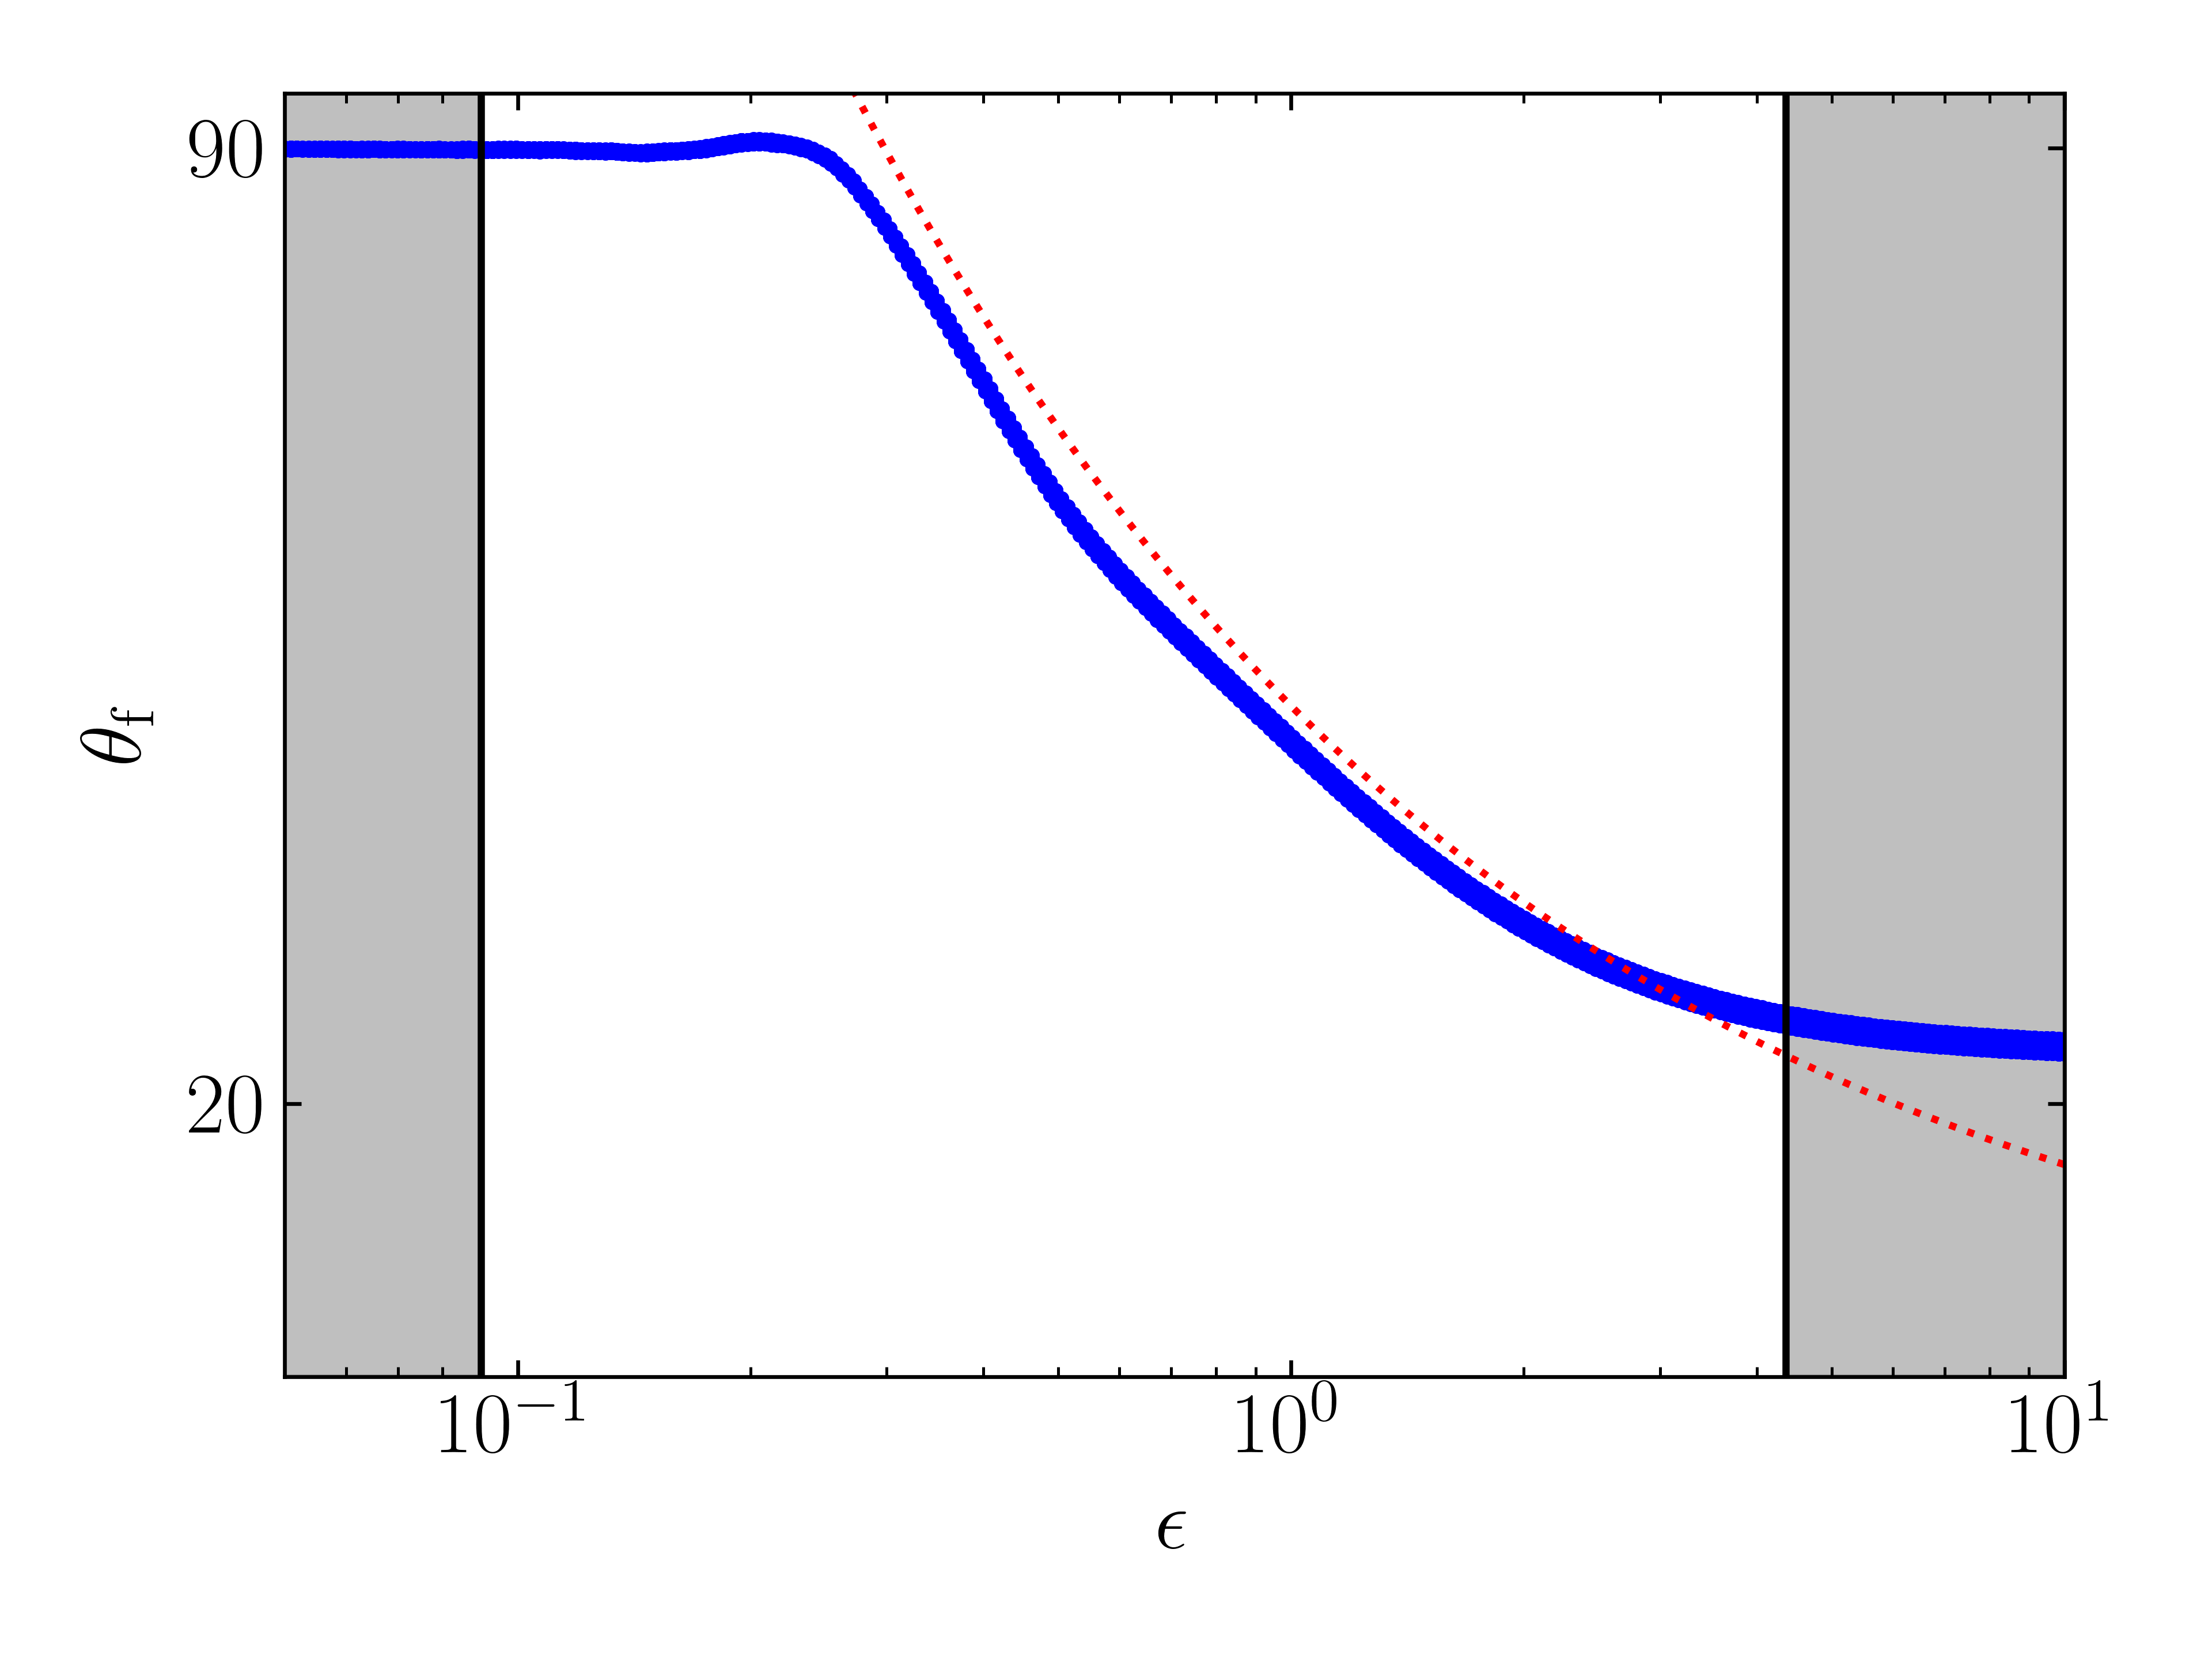
\includegraphics[width=\columnwidth]{../initial/2_toy2/3scan_20.png}
    \caption{Same as \autoref{fig:nonad_3_scan} but for $I=20^\circ$. Note that
    \autoref{eq:nonad_q_f} is accurate until $\theta_f \approx 90^\circ$, which
    occurs before the transition to the adiabatic
    regime.}\label{fig:nonad_3_scan_20}
\end{figure}

\bibliographystyle{mnras}
\bibliography{Su_sep_cross}

% \clearpage
% \onecolumn
\appendix

\section{Approximate Adiabatic Evolution}\label{s:app_transition}

In this section, we will use approximations valid for small $\eta$ to derive
analytic expressions for the final obliquities at small $\theta_{sd, i}$ and
associated probabilities for the $II \to I, II \to III$ tracks that are
accessible.

We first seek a simple parameterization for the separatrix. We first solve for
equilibria of the equation of motion \autoref{eq:dsdt_base} to compute the
coordinates for Cassini State 4:
\begin{equation}
    \cos \theta_4 \approx \frac{\mu \cos I}{1 - \eta \sin I}.
\end{equation}
Note that $\phi_4 = 0$. Then, the separatrix is the level curve of the
Hamiltonian intersecting CS4, so it satisfies $\mathcal{H}\p{\theta_{sep}(\phi),
\phi} = \mathcal{H}\p{\theta_4, \phi_4}$. This solves to be approximately
\begin{equation}
    \cos \theta_{sep}(\phi) \approx \cos \theta_4 \pm
        \sqrt{2\eta \sin I\p{1 - \cos \phi}}.
\end{equation}
Integration of the phase area enclosed by the two legs of the separatrix then
yields
\begin{equation}
    A_{II}(\eta) \approx 16\sqrt{\eta \sin I}.\label{eq:a_approx}
\end{equation}
This, in conjunction with \autoref{eq:henrard_hop}, is sufficient to compute
$\theta_f\p{\theta_{sd, i}}$ for zone $II$ initial conditions.

\begin{itemize}
    \item For a given $\theta_{sd, i}$, we know that if $\eta \to \infty$ then
        the trajectory executes simple libration about $\hat{l}_d$, and so $A =
        2\pi\p{1 - \cos \theta_{sd, i}} \approx \pi \theta_{sd, i}^2$. This
        then implies $\eta_\star$ must be the solution to $A_{II}(\eta_\star) =
        A$, or
        \begin{align}
            \eta_\star &\approx \p{\frac{2\pi\p{1 - \cos \theta_{sd,i}}}{
                        16}}^2 / \sin I,\nonumber\\
                    &\approx \p{\frac{\pi \theta_{sd, i}^2}{16}}^2/\sin I.
        \end{align}

    \item Upon separatrix encounter, a transition to either zone $I$ or zone
        $III$ occurs. These can be calculated to have associated probabilities
        (using the approximate area \autoref{eq:a_approx})
        \begin{align}
            \Pr_{II \Rightarrow I} &\approx \frac{2\pi
                \eta_{\star} \cos I + 4\sqrt{\eta_{\star}\sin
                I}}{8\sqrt{\eta_{\star}\sin I}},\\
            \Pr_{II \Rightarrow III} &\approx \frac{-2\pi
                \eta_{\star} \cos I + 4\sqrt{\eta_{\star}\sin
                I}}{8\sqrt{\eta_{\star}\sin I}}.
        \end{align}

    \item Upon a transition to zone $I$ or zone $III$, the final obliquities can be
        predicted by observing the final adiabatic invariant $A_f =
        -A_I(\eta_\star)$ in the zone $I$ case and $A_f = A_I(\eta_\star) +
        A_II(\eta_\star)$ in the zone $III$ case. As $\eta \to 0$, these
        correspond to obliquities
        \begin{align}
            \cos \theta_{f, II \Rightarrow I} &\approx
                \p{\frac{\pi \theta_{sp, i}^2}{16}}^2 \cot I
                    + \frac{\theta_{sp, i}^2}{4},\\
            \cos \theta_{f, II \Rightarrow III} &\approx
                \p{\frac{\pi \theta_{sp, i}^2}{16}}^2 \cot I
                    - \frac{\theta_{sp, i}^2}{4}.
        \end{align}
        These are the black dotted lines overplotted in
        \autoref{fig:ad_ensemble}.
\end{itemize}

\section{Derivation of Nonadiabatic Evolution}\label{s:nonad_app}

We present a single result, the derivation of \autoref{eq:nonad_q_f}. We take
\autoref{eq:dsdt_base} and choose coordinate axes such that $\hat{l} = \hat{z},
\hat{l}_d = \hat{z} \cos I + \hat{x}\sin I$, then we obtain
\begin{equation}
    \rd{\hat{s}}{t} = \s{
        \p{\eta \cos I - 1}\hat{z} + \eta \sin I \hat{x}} \times \hat{s}.
\end{equation}

Now, let's assume that $s_z \approx \cos I$ throughout the evolution of $\hat{s}$
(note that $\theta_{sd, i} = 0$ implies the initial $s_z = \cos I$). Then let's
examine the evolution of quantity $S = s_x + is_y$ instead:
\begin{equation}
    \rd{S}{t} = i\p{\eta\cos I - 1}S - i \eta \sin I\cos I.\label{eq:nonad_ode}
\end{equation}
Now this is a first-order ODE in $S$, albeit complex, which can be solved via
an integrating factor
\begin{align}
    \Phi(t) &\equiv \int_{-\infty}^t \p{1 - \eta(t') \cos I}
        \mathrm{d}t',\\
    \at{S(t) e^{i\Phi(t)}}_{-\infty}^t
        &= \int\limits_{-\infty}^t e^{i\Phi(t')}
            \p{-i\eta(t')\sin I\cos I}\;\mathrm{d}t'\label{eq:nonad_int}
\end{align}
We now invoke stationary phase, asserting that $e^{i\Phi(t)}$ is dominated by
its contribution where $\dot{\Phi} = 0$ (the phases add constructively). But
$\dot{\Phi} = 0$ is where $1 - \eta\cos I = 0$, or where $\eta\cos I = 1$.

Now at this point, let's choose $\eta(0) = 1/\cos I, \at{\rd{\eta}{t}}_{t=0} =
-\epsilon/\cos I$. Then we expand near $t = 0$ so
\begin{align*}
    \Phi(t) &\approx \Phi(0) + \frac{1}{2}\ddot{\Phi}t^2,\\
        &\approx \Phi(0) + \frac{1}{2}\epsilon t^2,\\
    \int\limits_{-\infty}^t e^{i\Phi(t')}\eta(t')\;\mathrm{d}t'
        &\approx
        \begin{cases}
            0 & t < 0,\\
            \frac{1}{\cos I}e^{i\Phi(0)}\int\limits_{-\infty}^\infty
                \exp\s{\frac{i}{2}\epsilon t^2}\;\mathrm{d}t
                & t > 0.
        \end{cases}\\
    \int\limits_{-\infty}^\infty
                \exp\s{\frac{i}{2}\epsilon t^2}\;\mathrm{d}t
        &= \int\limits_{-\infty}^\infty e^{-\tau^2}\;\mathrm{d}\tau
            \sqrt{\frac{2}{i\epsilon}},\\
        &= \sqrt{\frac{2\pi}{i\epsilon}}.
\end{align*}

Now, it should be noted that $e^{i\Phi}$ is just a phase; all we really care
about is $\abs{S} = \sqrt{1 - s_z^2}$. Thus, taking the absolute value of both
sides of \autoref{eq:nonad_int}, assuming $S\p{-\infty} \ll S\p{+\infty}$ and
noting $\theta_f \approx \abs{S}(+\infty)$, we obtain
\begin{equation}
    \theta_f = \tan I\cos I\sqrt{\frac{2\pi}{\epsilon}}.\label{eq:nonad_dong}
\end{equation}

It should be noted that this calculation breaks down in two ways:
\begin{itemize}
    \item If the evolution of $\hat{s}$ is adiabatic, then it is invalid to
        assume $s_z$ is approximately constant in time, as many
        circulation/libration orbits can ensue. Only when the driving is
        sufficiently impulsive that the evolution dominates the change in $s_z$
        is this calculation valid.

    \item If $\abs{S\p{-\infty}} \sim \abs{S\p{+\infty}}$, then taking the
        absolute value of both sides of \autoref{eq:nonad_int} no longer simply
        yields $\abs{S}\p{+\infty}$. This corresponds to the extreme limit
        where $\eta$ changes so suddenly that $\hat{s}$ has no time to respond
        and remains roughly unchanged as $\eta \to 0$. This is accommodated by
        noting $\theta_f \geq \theta_{sd, i}$, so the correct estimate can be
        roughly amended
        \begin{equation}
            \theta_f \simeq \min\p{\tan I\cos I\sqrt{\frac{2\pi}{\epsilon}},
                \theta_{sd, i}}.
        \end{equation}
\end{itemize}

\label{lastpage} % chktex 24
\end{document}
